\section{Motivation}

Building upon the discussion of $t\bar{t}H$ production in the previous chapter, an essential question concerns the $CP$ structure of the Higgs boson couplings. 
In the SM the Higgs boson is a scalar particle and its interactions with fermions and vector bosons are purely $CP$-even. 
The hypothesis of a purely pseudoscalar state with $CP$-odd interactions has already been excluded by existing measurements~\cite{ATLAS:2015yey,CMS:2014quz,ATLAS:2022ers,CMS:2022dbx}. 
Nevertheless, it remains experimentally viable that the Higgs boson is a $CP$-mixed state, arising naturally in extended Higgs sectors. 
Such a scenario would provide a new source of $CP$ violation beyond the SM, which is of particular interest since additional $CP$-violating effects are required to explain the observed baryon asymmetry of the Universe (explained in Section~\ref{sec:BSM}). 

Studies of the coupling between the Higgs boson and the top quark cans sheed light on this possibility~\cite{Gunion:1996xu, Ellis:2013yxa, He:2015spx, Boudjema:2015nda}. 
While the inclusive cross-section of $t\bar{t}H$ is primarily sensitive to the absolute strength of the top-quark Yukawa coupling, the $tH$ process is directly affected by the relative phase between the Higgs couplings to the top quark and to the $W$ boson. 
A simultaneous study of $t\bar{t}H$ and $tH$ therefore provide sensitivity to potential $CP$ violation in the top-Higgs interaction. 

This can be expressed in a convenient and model-independent way by extending the SM Lagrangian of the top-Higgs interaction vertex ($\Ht\bar{t}$) to include a $CP$-mixing angle $\alpha$~\cite{Demartin_2014}:
\begin{equation}
{\cal L}_{Ht\bar{t}}=-\kappa' \, y_t \, \phi \, \bar{\psi_t}(\cos{\alpha} + i\gamma_5\sin{\alpha})\psi_t\,,
\end{equation}
where $\kappa'$ is a coupling modifier and $\alpha$ interpolates between a pure scalar ($\alpha=0$) and a pure pseudoscalar interaction ($\alpha=\pi/2$). 
In this framework, both $t\bar{t}H$ and $tH$ cross-sections depend on $\alpha$, as shown in Fig.~\ref{fig:th_cp_dependence}. 

\begin{figure}[htbp]
  \centering
  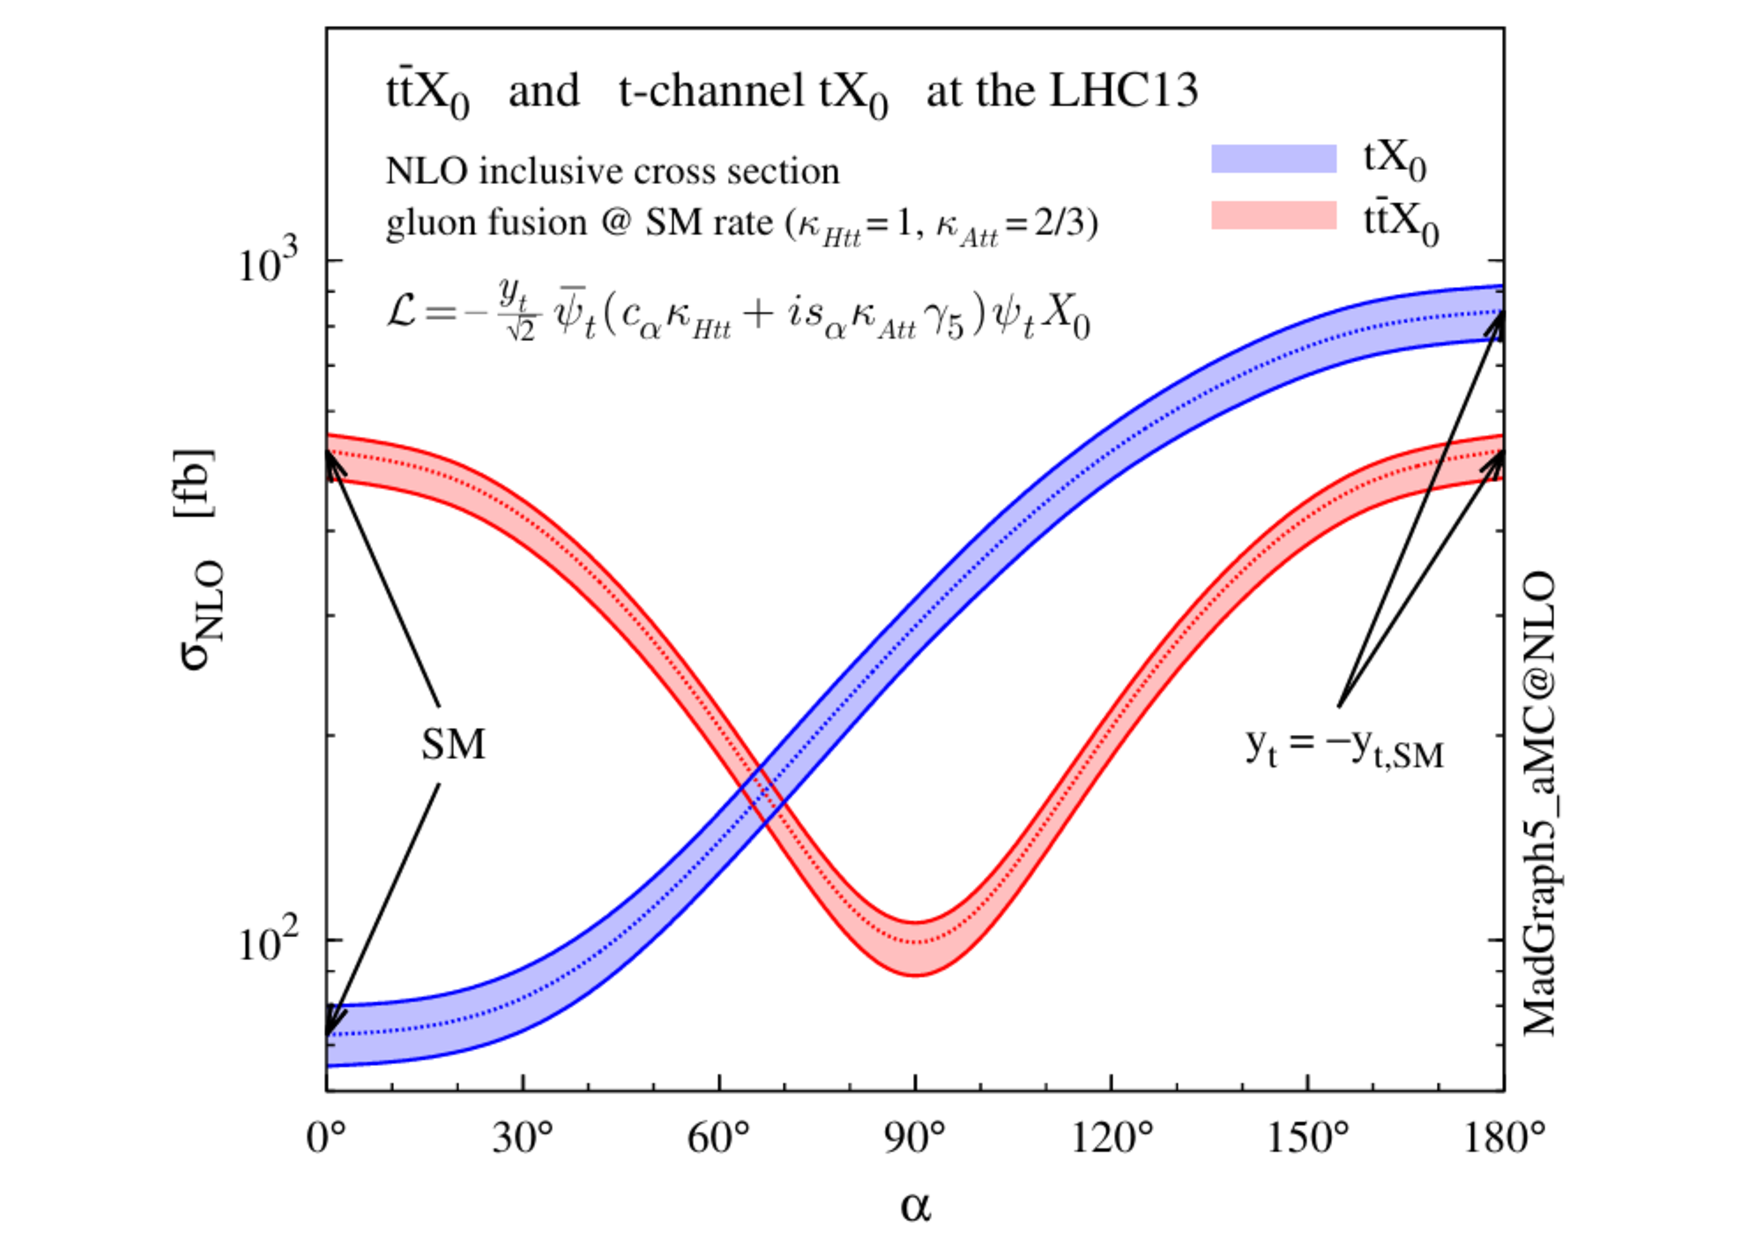
\includegraphics[width=0.65\textwidth]{cp_higgs.pdf}
  \caption{NLO cross-sections for $t\bar{t}H$ and $tH$ production (where $X_{0}$ denotes the Higgs boson) at $\sqrt{s}=13$~TeV as a function of the $CP$-mixing angle $\alpha$, with scale uncertainties included~\cite{demartin2015}.}
  \label{fig:th_cp_dependence}
\end{figure}

With the current precision of about 20\% in the \ttH\ measurement, phases up to $\alpha \sim 30^{\circ}$ are still compatible with data. 
Such values would naturally imply observable deviations from the SM prediction in $tH$ production, providing a strong motivation for a combined measurement of $tH$ and \ttH\ to test the $CP$ structure of the top-Higgs interaction.
The pure $CP$-odd hypothesis ($\alpha = 180^{\circ}$) has been also excluded experimentally~\cite{thgammagamma}.

The production of a Higgs boson with a single top quark proceeds through the electroweak interaction, with three contributing modes: the $t$-channel ($tHqb$), the $s$-channel ($tHb$), and the associated production with a $W$ boson ($tWH$)~\cite{demartin2015,Demartin_2017}. These processes are distinguished by the way the Higgs boson couples either to the top quark or to the $W$ boson, leading to characteristic interference patterns that are sensitive to the value of $\alpha$. 
The corresponding Feynman diagrams for the different $tH$ modes are shown in Figures~\ref{fig:feynman_tH_t}-\ref{fig:feynman_tWH}.

\begin{figure}[!htbp]
  \centering
  \begin{subfigure}[b]{0.4\textwidth}
    \centering
    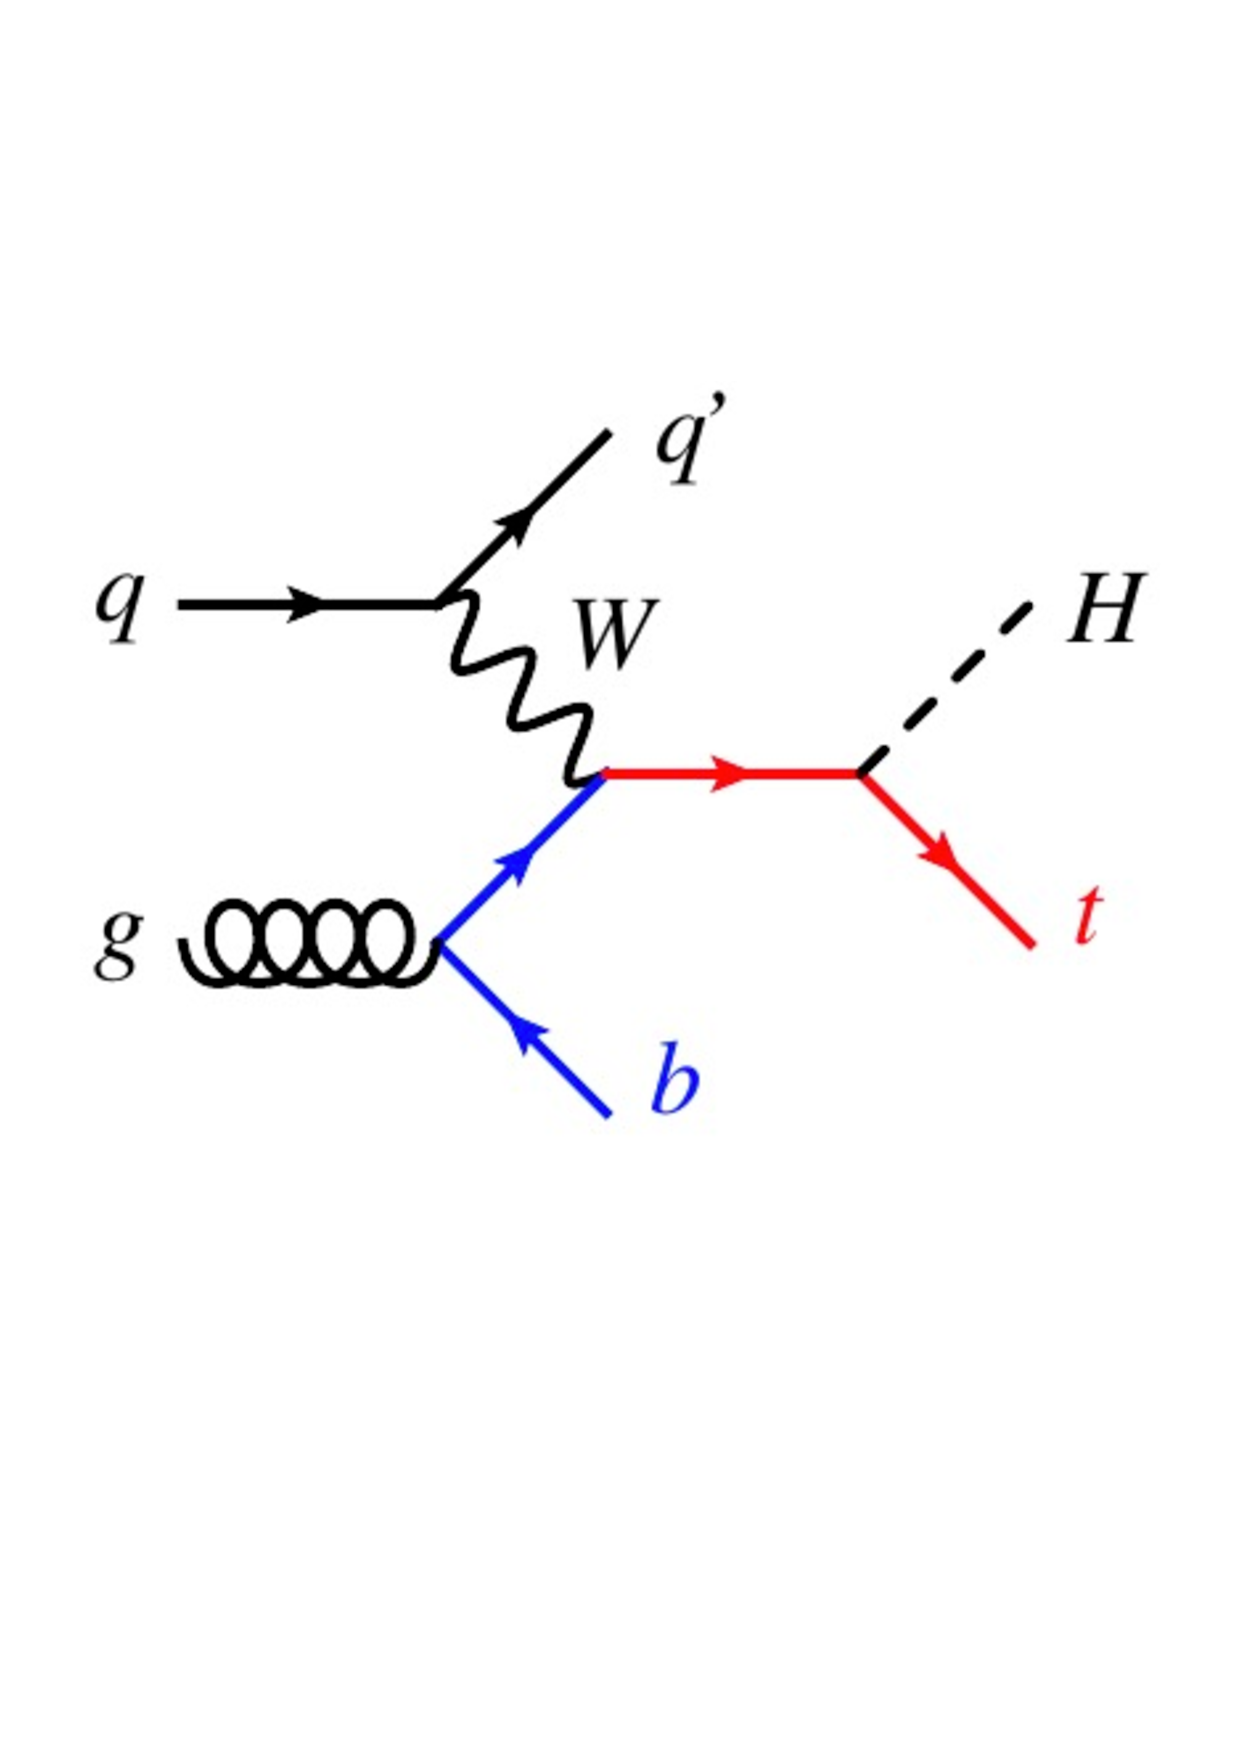
\includegraphics[width=\textwidth]{thqb_t.pdf}
  \end{subfigure}
  \begin{subfigure}[b]{0.4\textwidth}
    \centering
    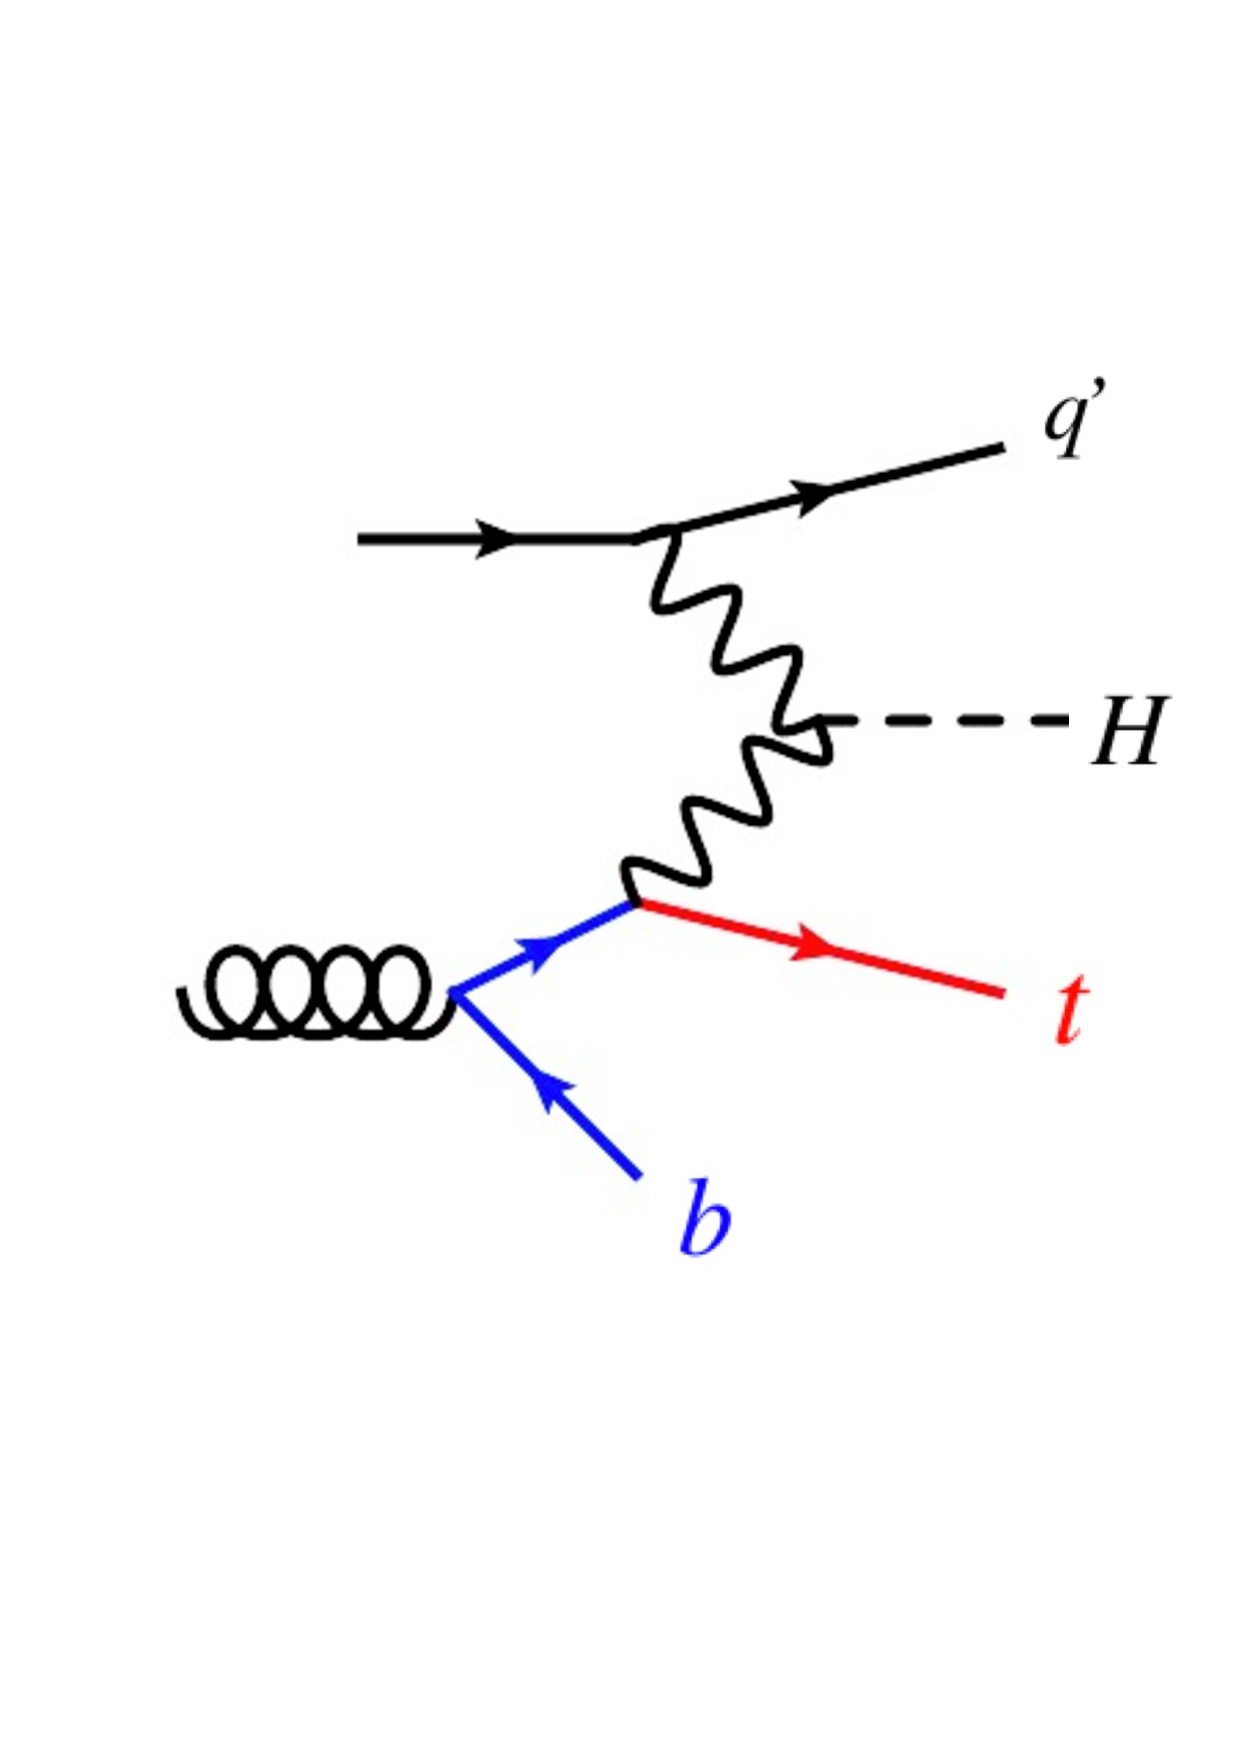
\includegraphics[width=\textwidth]{thqb_t_2.pdf}
  \end{subfigure}
  \caption{Representative leading-order Feynman diagrams for $tHqb$ in the $t$-channel~\cite{Barger_2010}.}
  \label{fig:feynman_tH_t}
\end{figure}


\begin{figure}[!htbp]
  \centering
  \begin{subfigure}[b]{0.4\textwidth}
    \centering
    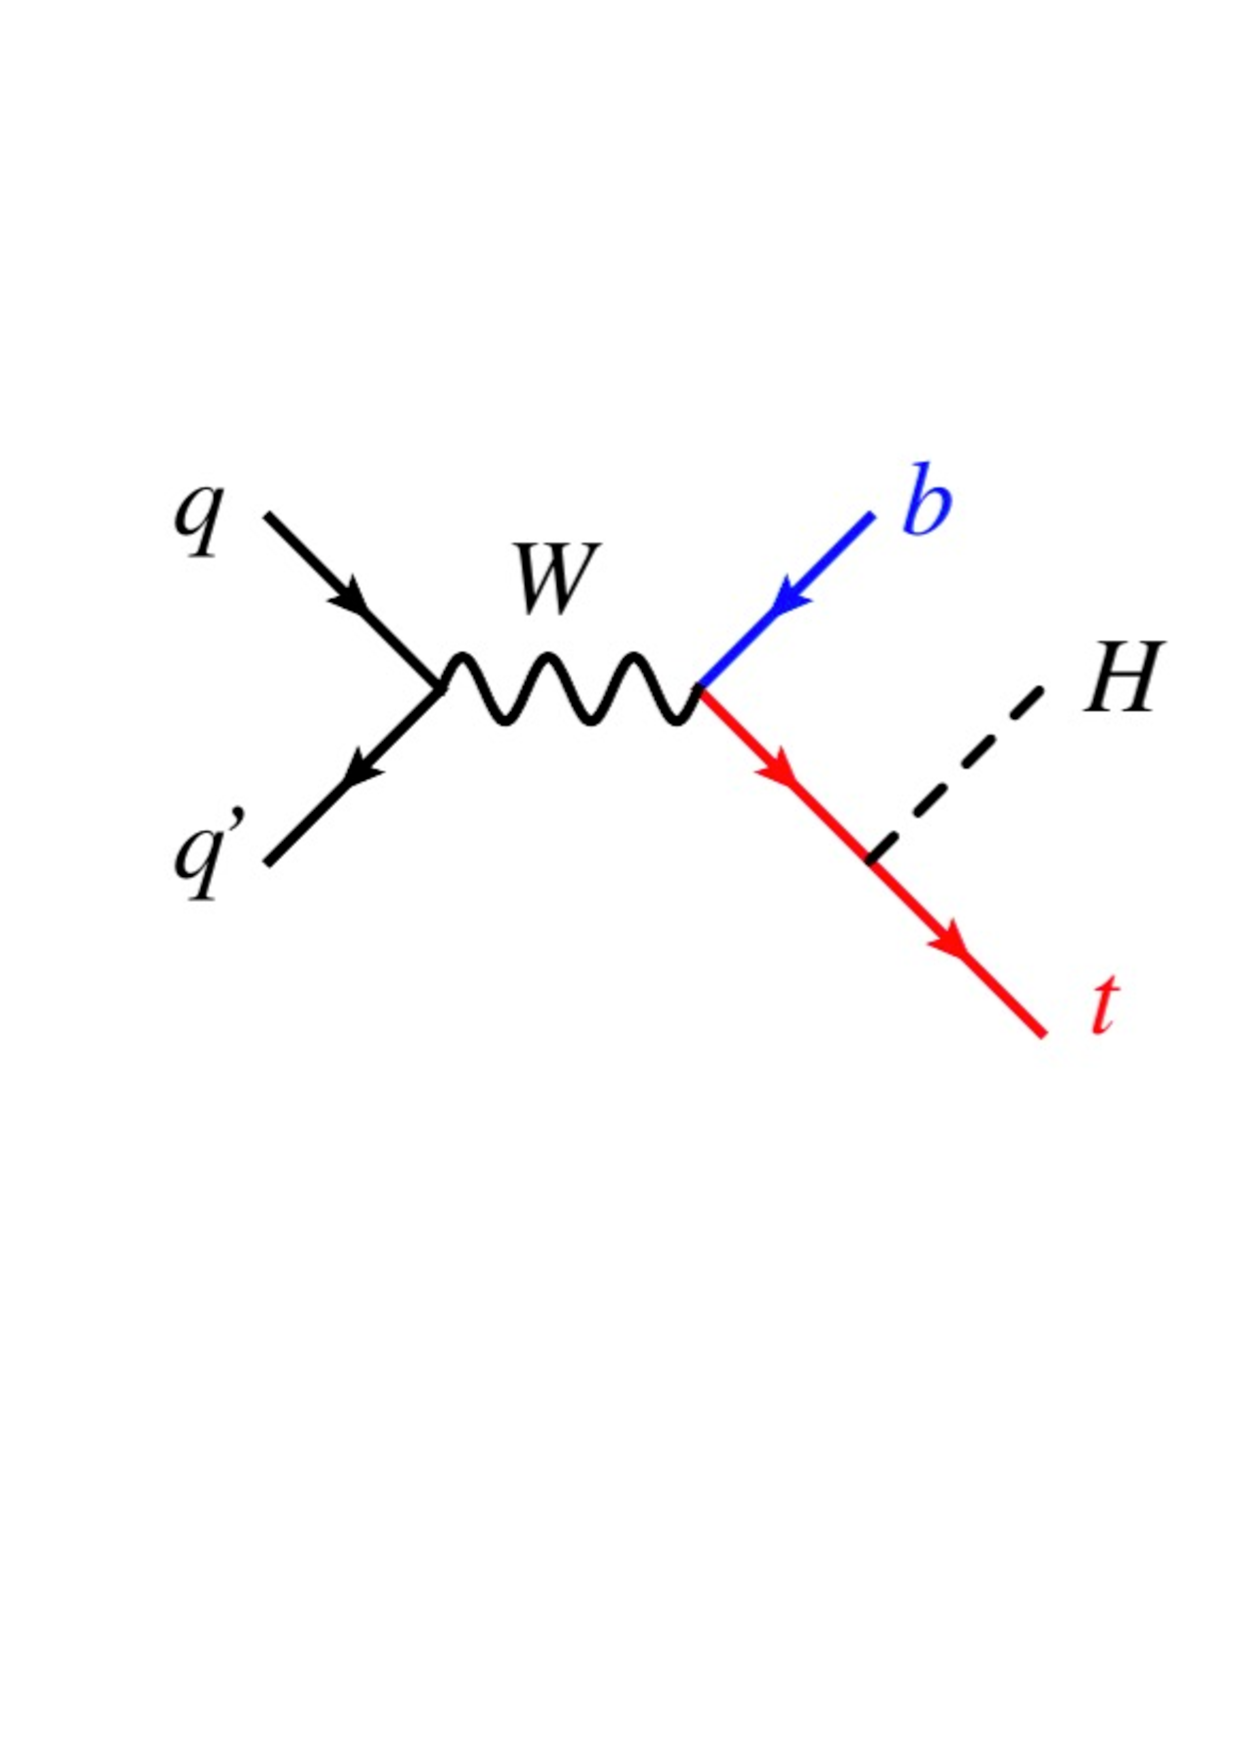
\includegraphics[width=\textwidth]{thqb_s.pdf}
  \end{subfigure}
  \begin{subfigure}[b]{0.4\textwidth}
    \centering
    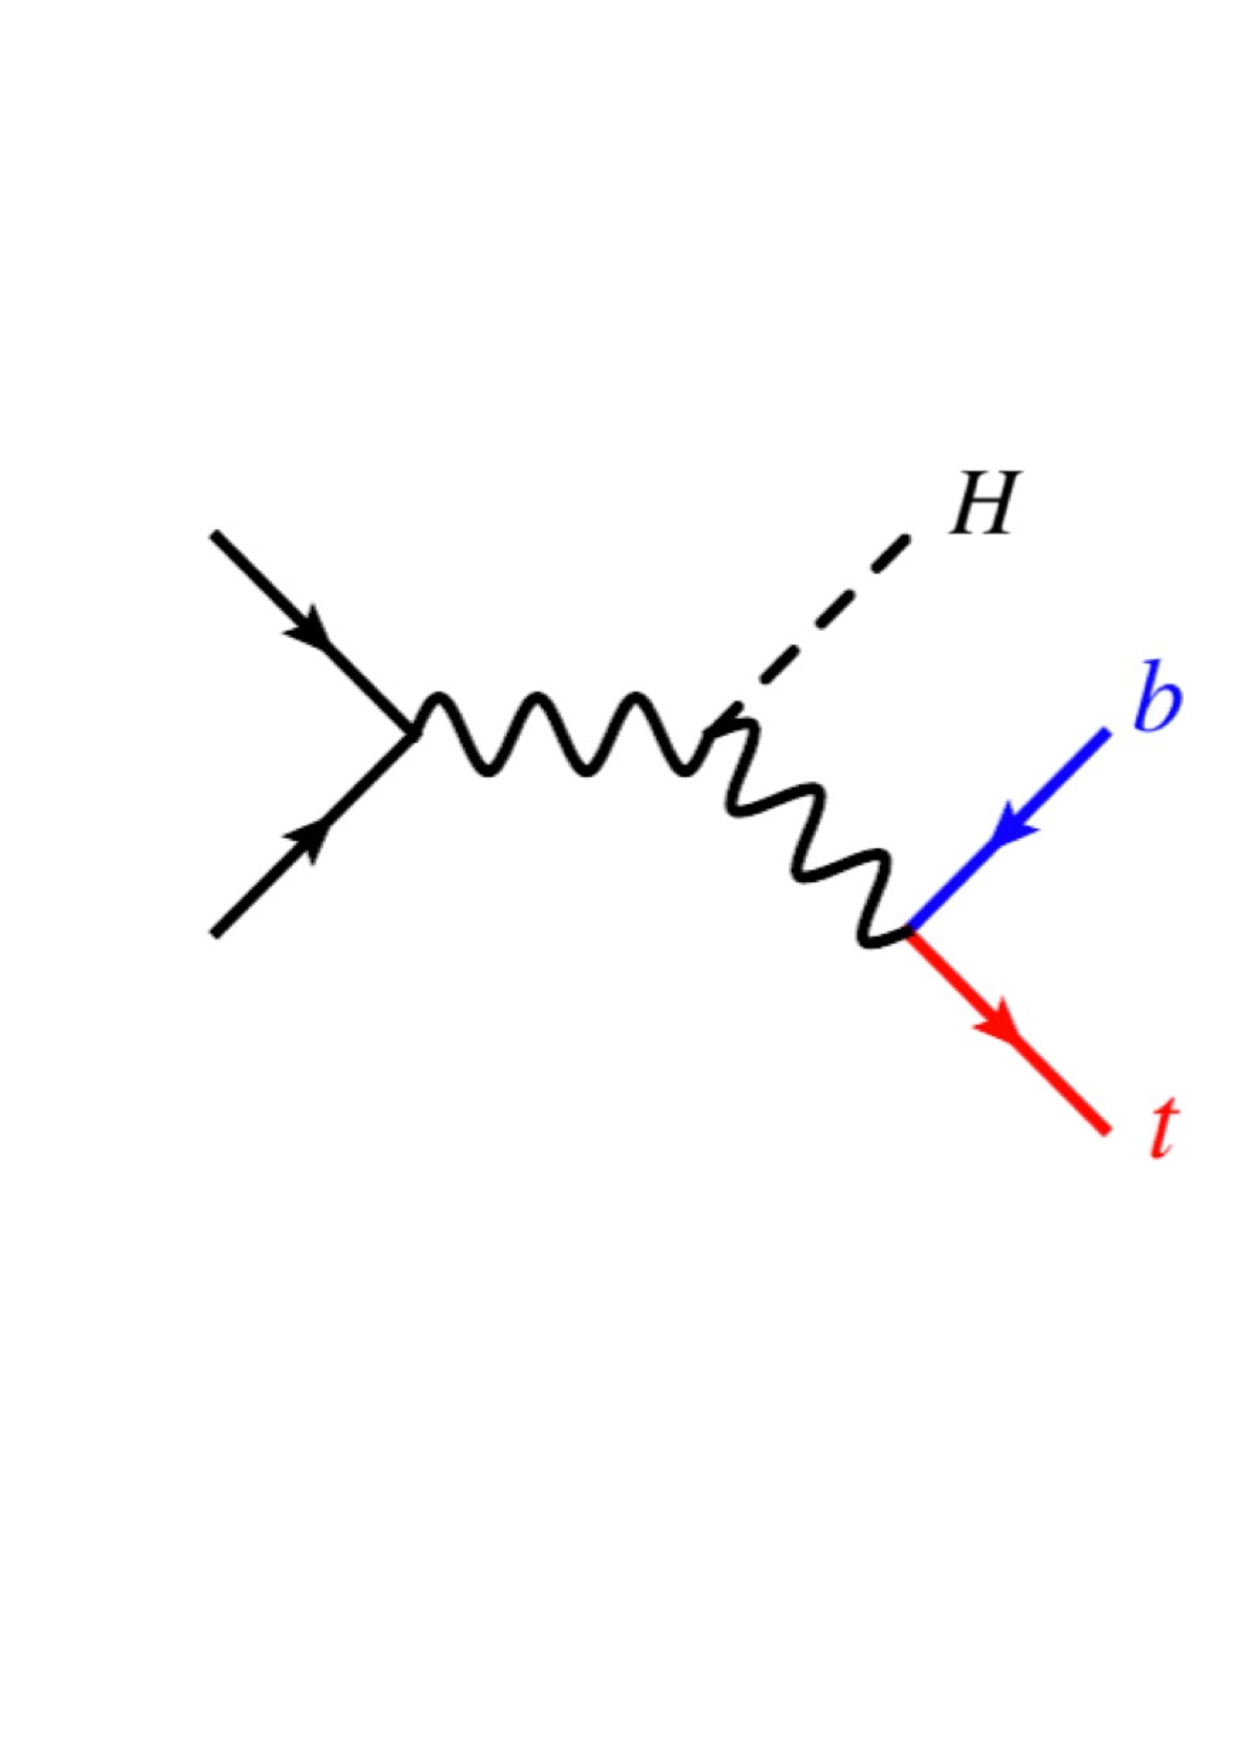
\includegraphics[width=\textwidth]{thqb_s_2.pdf}
  \end{subfigure}
  \caption{Representative leading-order Feynman diagrams for $tHqb$ in the $s$-channel~\cite{Barger_2010}.}
  \label{fig:feynman_tH_s}
\end{figure}

\begin{figure}[!htbp]
  \centering
  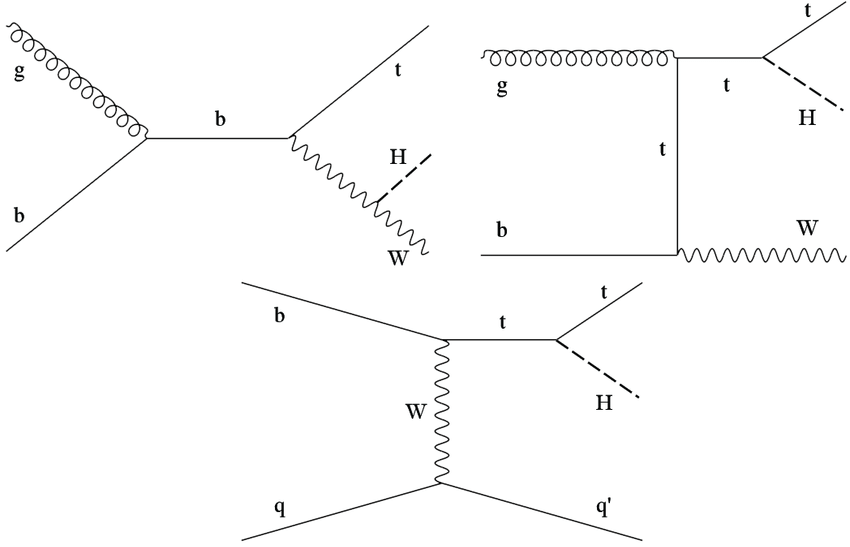
\includegraphics[width=0.6\textwidth]{twh.png}
  \caption{Representative leading-order Feynman diagrams for $tWH$~\cite{twh}.}
  \label{fig:feynman_tWH}
\end{figure}

Among these, the $t$-channel dominates, with a predicted cross-section of about $74$~fb at $\sqrt{s}=13$~TeV, compared to $15$~fb for $tHW$ and less than $3$~fb for the $s$-channel. The $s$-channel remains negligible due to its very small rate, while the $tHW$ process, although larger, is experimentally treated as a background in most of searches for \thqb because of its topology is more similar to \ttH. Consequently, the $tHqb$ process provides the cleanest handle on the $CP$ structure of the top-Higgs interaction, especially when studied in conjunction with $t\bar{t}H$ production in the fully hadronic $H \to \tau \tau$ final state.

The $tHqb$ event topology is characterised by two heavy objects, a top quark and a Higgs boson, accompanied by an energetic forward light-flavour quark and, typically, an additional low-$p_{T}$ (\textit{soft}) $b$-quark arising from gluon splitting.\footnote{In this context, ``soft'' refers to the comparatively low transverse momentum of the extra $b$-quark, which is often below the jet selection thresholds or reconstructed as a central, less-energetic jet. As a consequence, the $tHqb$ topology usually contains only one $b$-jet from the top-quark decay, in contrast to the $t\bar{t}H$ process which features two energetic $b$-jets.}
  The top-quark and Higgs-boson systems are typically produced in the central region of the detector, recoiling against each other. 
  In contrast, $tWH$ production features three heavy objects in the final state: the top quark, a $W$ boson, and a Higgs boson, together with a typically soft $b$-quark from gluon splitting. 
  This topology closely resembles $t\bar{t}H$ production and results in an identical final state, making it difficult to disentangle from the $t\bar{t}H$ contribution and therefore justifying its treatment as a background in this analysis. 
  
  Single-top Higgs production has not been observed yet.
  The CMS Collaboration has reported upper limits on the $tH$ rate in both multi-lepton and $b\bar{b}$ final states. 
  In the multi-lepton channel, the measured signal strength was found to be 
  \[
  \mu_{tHqb+tWH} = 5.1 \pm 2.7~(\text{stat.}) \pm 3.0~(\text{syst.})~\cite{Sirunyan_2021},
  \] 
  while in the $b\bar{b}$ channel cross-sections up to 14.6 times the SM prediction were excluded at 95\% confidence level~\cite{2025}. 
  The most recent ATLAS search~\cite{ATLAS:2025irr}, targeting $H\to b\bar{b}$, $H\to WW^*$, $H\to ZZ^*$, and $H\to\tau\tau$ decays in events with an isolated lepton from the top quark, reports a measured signal strength of
  \[
  \mu_{tHqb+tWH} = 8.1 \pm 2.6~(\text{stat.}) \pm 2.0~(\text{syst.}),
  \] 
  corresponding to a 2.8\,$\sigma$ observed (0.4\,$\sigma$ expected) significance above the background only hypothesis. 
  The observed (expected) 95\% confidence level upper limit on the $tH$ cross-section was $13.9$ ($6.1$) times the SM prediction. 
  This represents the most stringent constraint on $tH$ production to date, while still allowing for possible deviations from the SM.  
  
  In addition, ATLAS has performed searches in the $H \to \gamma\gamma$ final state in top-associated Higgs production~\cite{thgammagamma}, which provide complementary sensitivity due to the excellent diphoton mass resolution and clean signal signature. 
  In that analysis, the measured signal strength for $tH$ production was found to be
  \[
  \mu_{tH} = 3^{+4}_{-3}~(\text{stat.}) \pm 1~(\text{syst.}).
  \]    
  In this context, the hadronic di-$\tau$ final state provides an attractive and complementary probe of both $t\bar{t}H$ and $tHqb$ production. 
  In particular, no ATLAS analysis has yet targeted the $tHqb$ channel in the fully hadronic $\tau\tau$ mode. 
  Moreover, a combined measurement is especially well motivated given that, due to their similar topology, $t\bar{t}H$ and $tHqb$ share the same dominant backgrounds, namely $Z\to\tau\tau$+jets and $t\bar{t}$. 
  Such a joint analysis becomes feasible for the first time thanks to the larger dataset now available combining the full Run-2 dataset with the new Run-3 data.
  This increase in luminosity, together with the adoption of improved object reconstruction and identification techniques, opens the possibility to explore $tHqb$ production in the $H\to\tau_{\mathrm{had}}\tau_{\mathrm{had}}$ final state while simultaneously refining the measurement of $t\bar{t}H$.
  



\section{Analysis overview}

In this new study, the full Run-2 dataset is employed, corresponding to an integrated luminosity of $140$~fb$^{-1}$ at a centre-of-mass energy of $\sqrt{s}=13$~TeV, reprocessed with ATLAS software release 22. 
This dataset has been complemented with the Run-3 data collected to date, corresponding to an additional $166$~fb$^{-1}$ of luminosity from the years 2022-2024 of data taking, at a centre-of-mass energy of $\sqrt{s}=13.6$~TeV.

Nevertheless, single-top Higgs production still suffers from low acceptance, particularly within the restricted phase space targeted in the previous $t\bar{t}H(\tau\tau)$ analysis presented in Chapter~\ref{chap:htautau}. 
For \thtt, the jet and $b$-jet selection must be relaxed as this process yields 5 jets, of which two are expected to be $b$-tagged. 
Furthermore, with the release 22 of ATLAS software, novel identification algorithms have been introduced, including \textsc{gntau} for $\tau$-lepton reconstruction and \textsc{gn2} for flavour tagging of jets. 
These improvements, together with a refined MVA strategy, allow the analysis to maintain a good balance between efficiency and background rejection, even under looser jet requirements. 
The updated BDT strategy now targets two signal processes, $t\bar{t}H$ and $tHqb$, against the dominant backgrounds, $Z\to\tau\tau$+jets and $t\bar{t}$. 
It is also important to highlight that, for process discrimination, the topology of $tHqb$ exhibits a distinctive feature: the spectator jet from the hard scatter tends to be very forward, as it carries a large fraction of the longitudinal momentum of the initial-state valence quark. This provides a clear signature of $tHqb$, which is absent in $t\bar{t}H$, where the leading jets originate from the two top quarks and therefore populate the more central region of the detector, as shown in Figure~\ref{fig:feynman_tH_ttH}.
\begin{figure}[htbp]
    \centering
    \begin{subfigure}[b]{0.37\textwidth}
      \centering
      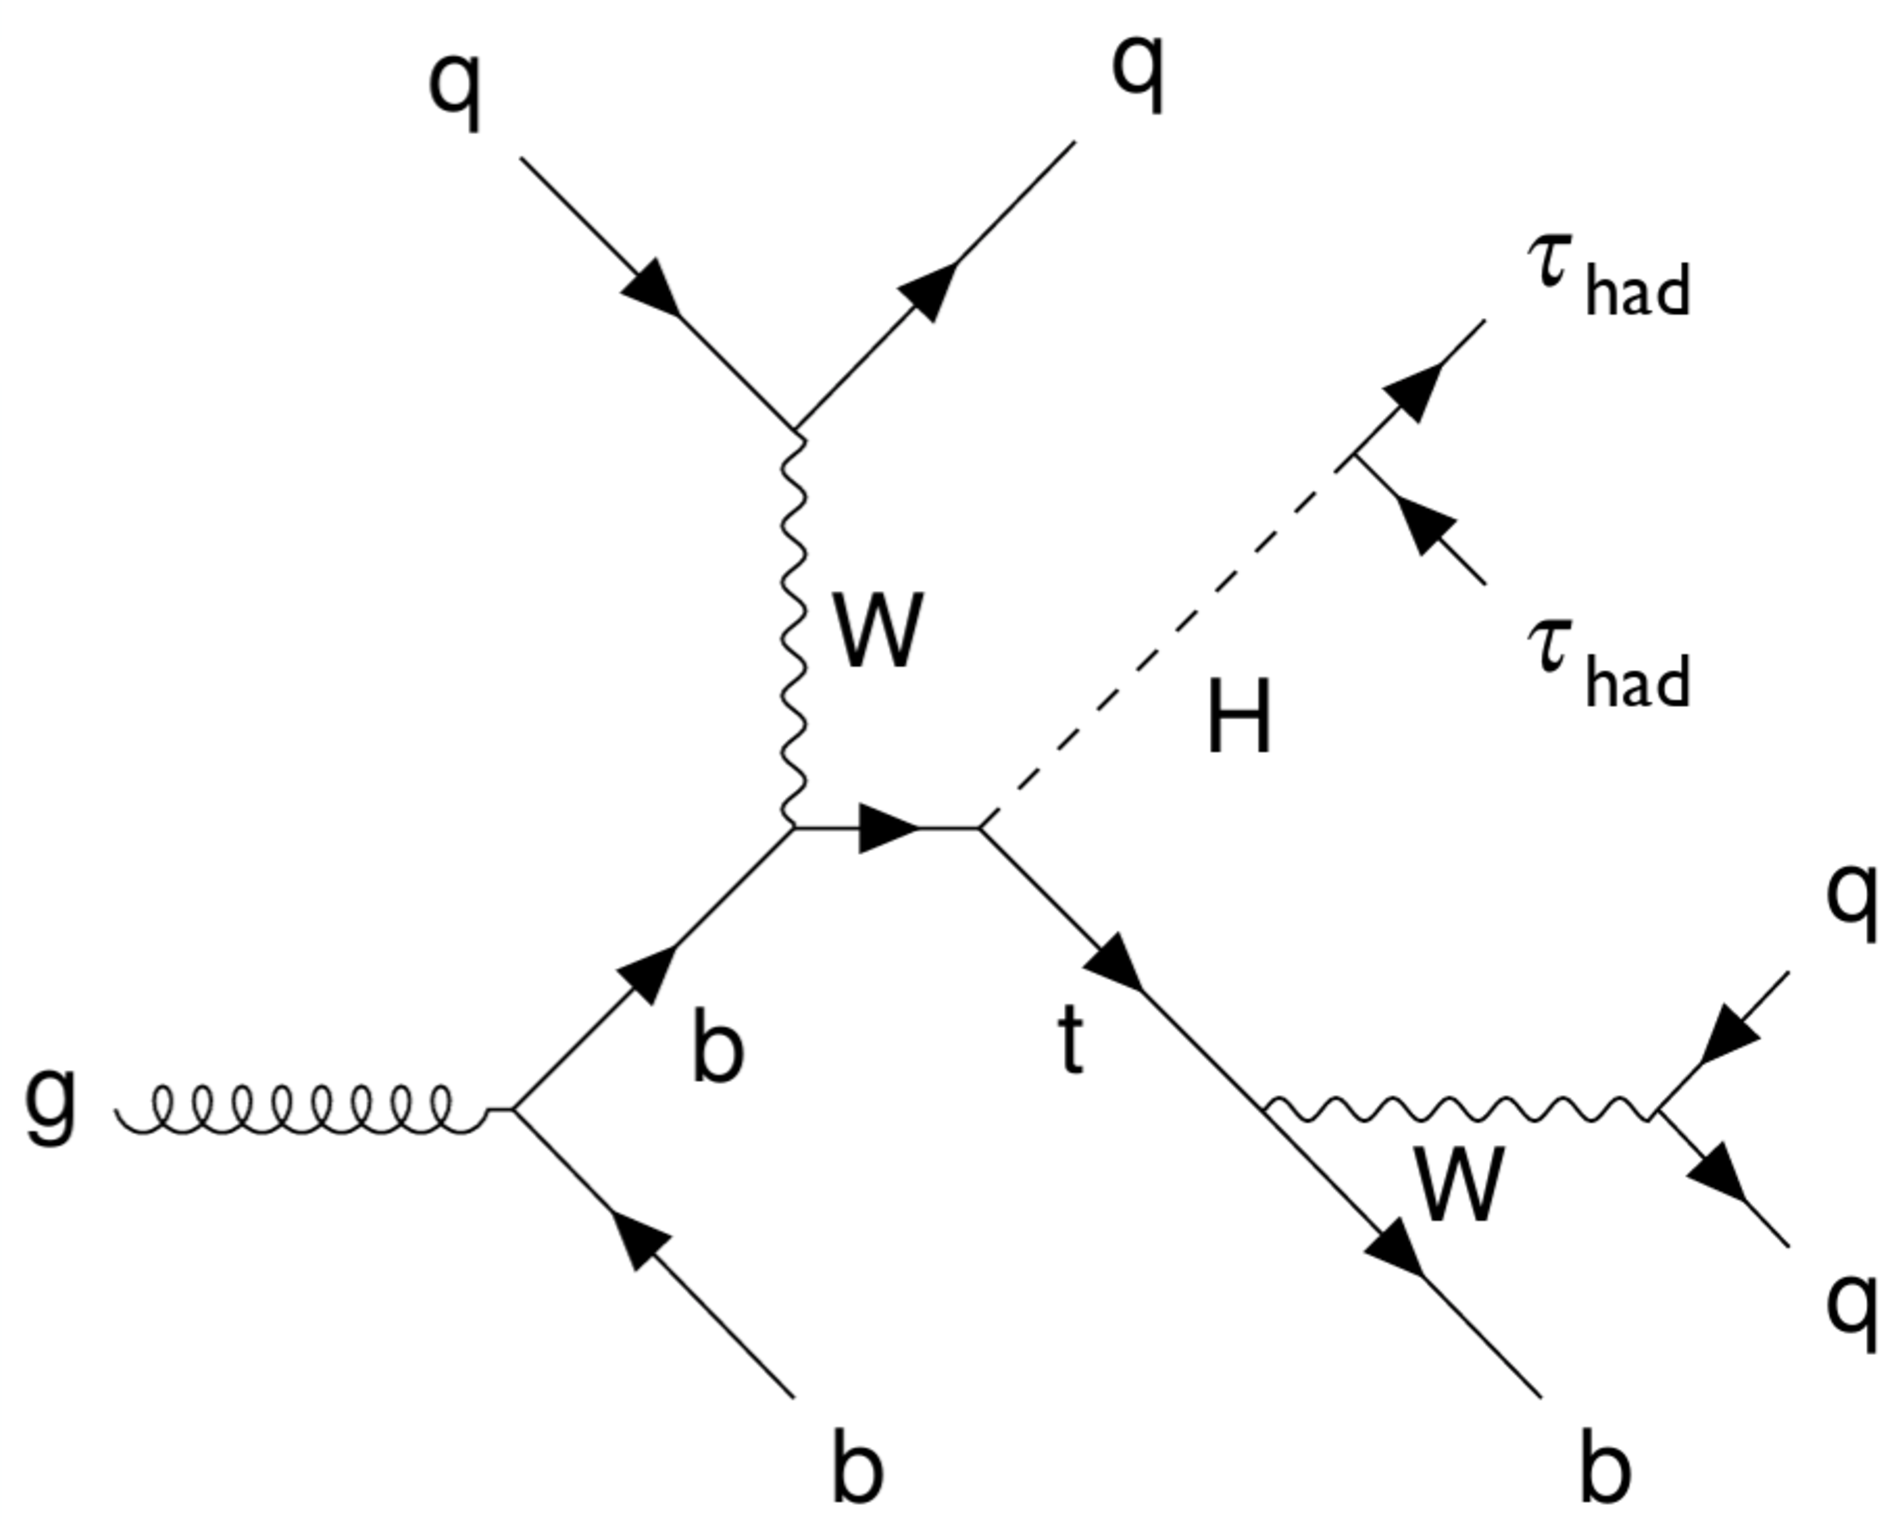
\includegraphics[width=\textwidth]{thqbtautau.pdf}
      \caption{}
    \end{subfigure}
    \begin{subfigure}[b]{0.4\textwidth}
      \centering
      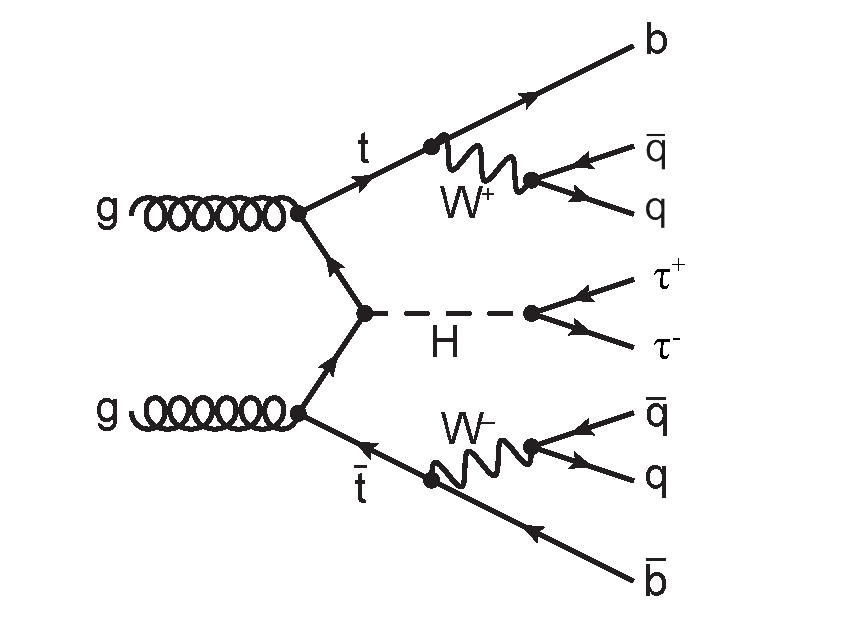
\includegraphics[width=\textwidth]{tth_diagram_1}
      \caption{}
    \end{subfigure}
    \caption{Representative leading-order Feynman diagrams for (a) $tH(\tau\tau)qb$ in the $t$-channel~\cite{Barger_2010} and (b) \ttHtt.}
    \label{fig:feynman_tH_ttH}
  \end{figure}

The study presented here constitutes the first attempt within ATLAS to perform a simultaneous measurement of both processes in the fully hadronic $\tau\tau$ final state. 
This chapter does not primarily aim at refining the $t\bar{t}H$ cross-section measurement, but to study and quantify the sensitivity that can be achieved for $tHqb$ production using the additional Run-3 data. 
For this reason, no STXS interpretation is attempted here and the results are expressed in terms of expected sensitivity derived from a statistical fit to pseudo-data samples, combined with real collision data in background-enriched control regions. 
As in the previous analysis, the main backgrounds are modelled with MC simulation and normalised to data through the fit, while fake-$\tau$ contributions are estimated with a fully data-driven fake-factor method. 

It is worth noting that for the Run-3 MC simulations of \ttbar and \ztautau significant mismodellings with respect to data are observed, particularly in the latter due to the change of generator version, as already discussed in Section~\ref{subsec:higgs_mc}. 
Following the same strategy, these discrepancies are ultimately corrected by dedicated normalization factors (NFs) that constrain and adjust the normalization of these backgrounds using data in the statistical fit. 
Nevertheless, in order to demonstrate that the overall agreement of the various observables between MC and data is under control, the \ttbar and \ztautau MC samples are rescaled by global factors of 1.2 and 1.4, respectively, in all prefit distributions (unless otherwise stated). 
As will be shown later in Section~\ref{statistical_th_tth}, the normalization factors extracted from the statistical fit are consistent with these estimates. 
For illustration, in Figure~\ref{mmc_scaled} it is shown the distribution of \mmc in Run-3, before and after applying these scalings.

\begin{figure}[htbp]
    \centering
    \begin{subfigure}[b]{0.49\textwidth}
      \centering
      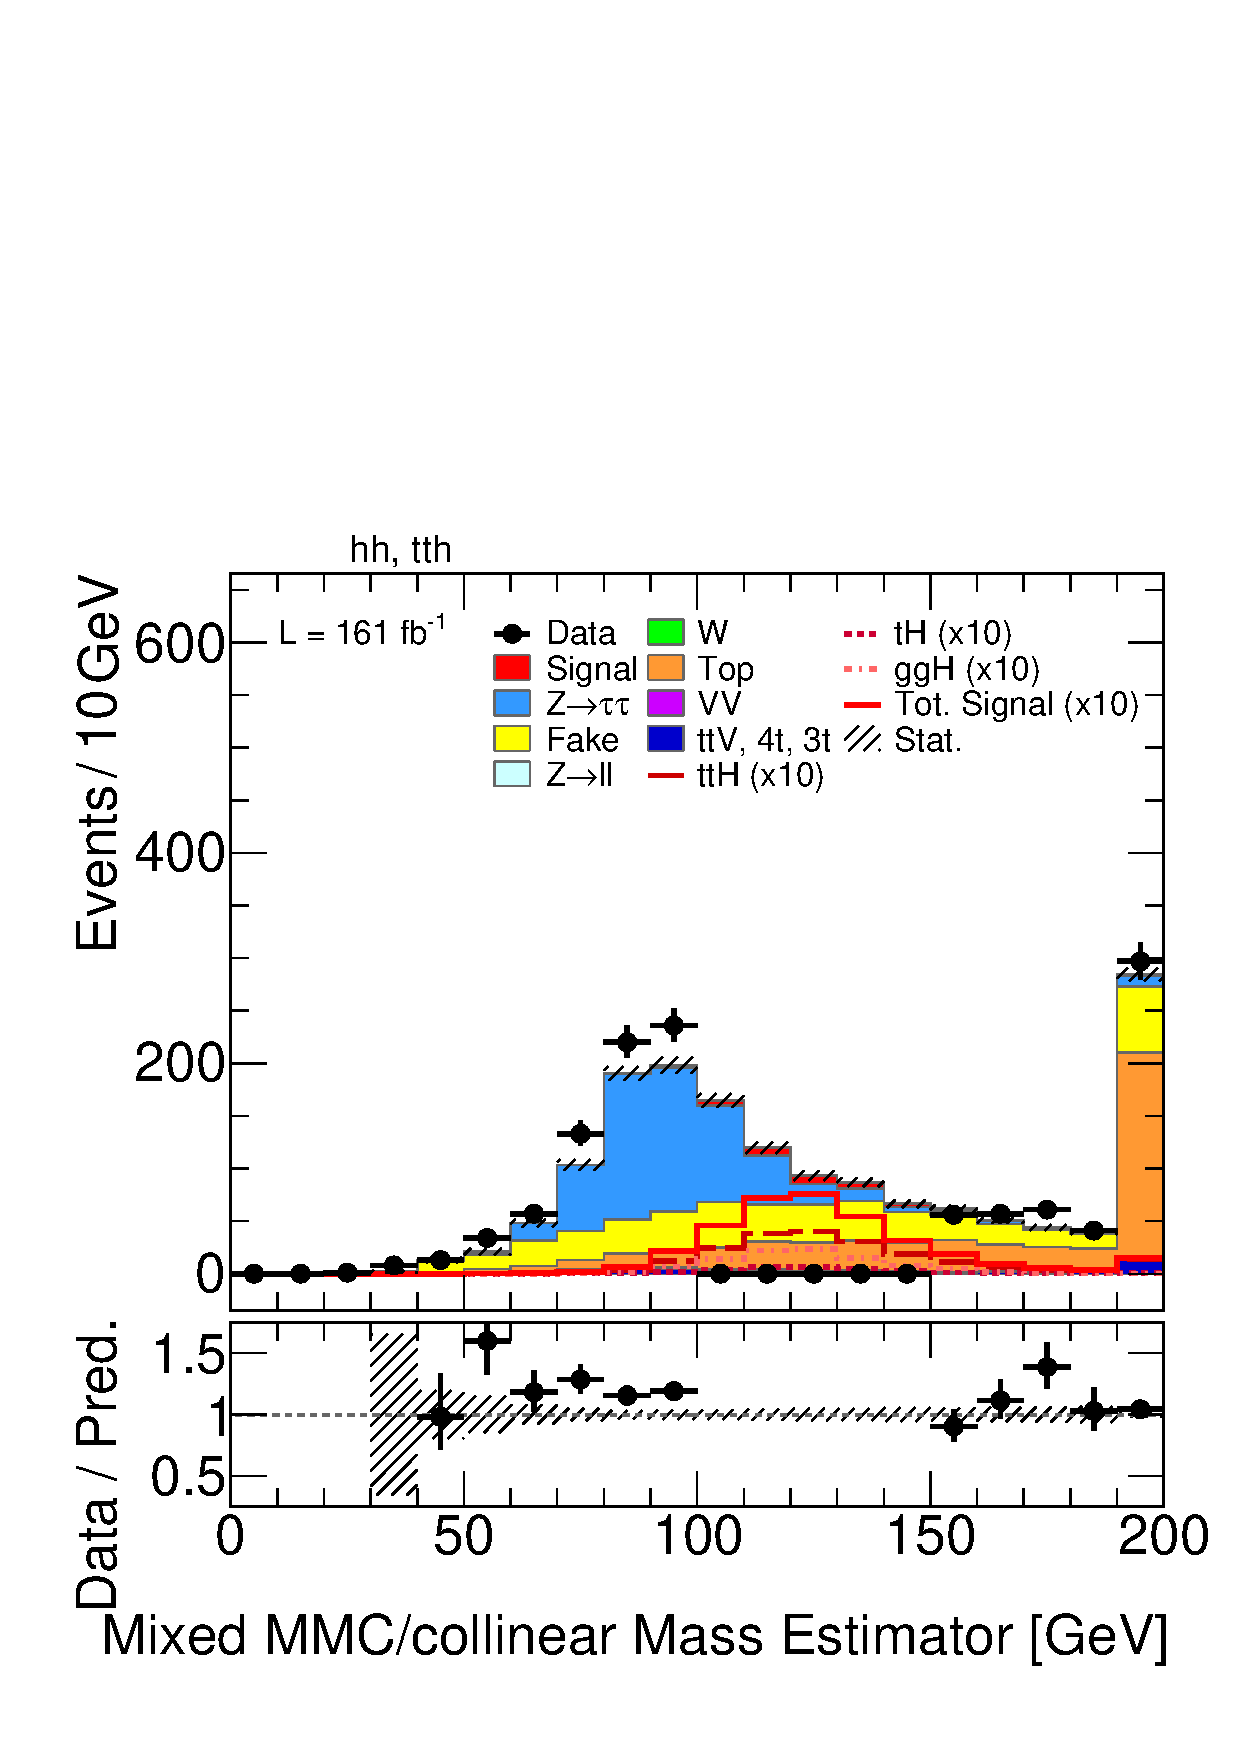
\includegraphics[width=\textwidth]{noscaled_plot_ditau_mmc_mlm_m_fix_hh_tth_22_23_24.pdf}
      \caption{}
    \end{subfigure}
    \hfill
    \begin{subfigure}[b]{0.49\textwidth}
      \centering
      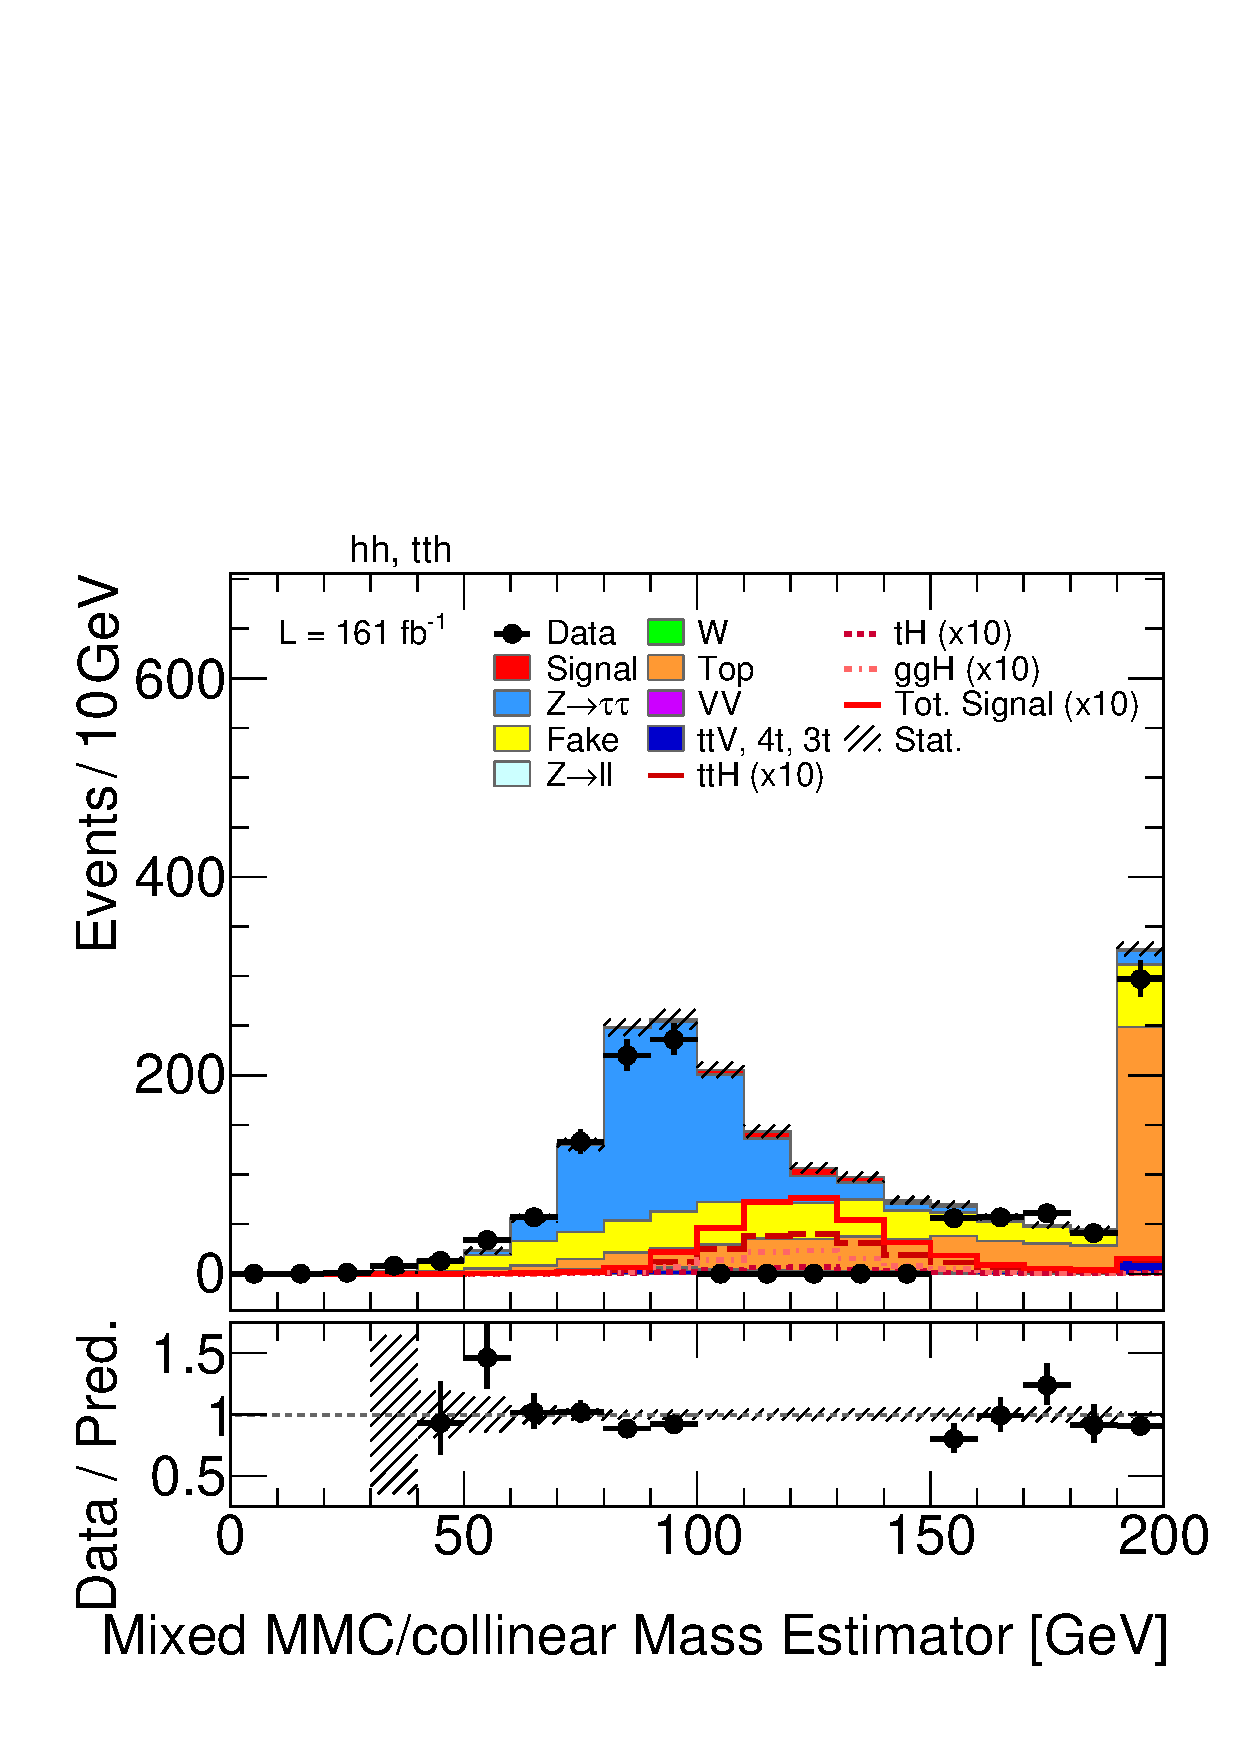
\includegraphics[width=\textwidth]{scaled_plot_ditau_mmc_mlm_m_fix_hh_tth_22_23_24.pdf}
      \caption{}
    \end{subfigure}
    \caption{
      Distribution of \mmc at preselection level in Run~3, with the region $100<$\mmc$<150$~GeV blinded in data. 
      The comparison between data and MC is shown (a) without applying any rescaling and (b) after rescaling the \ttbar and \ztautau MC samples by factors of 1.2 and 1.4, respectively. Only statistical uncertainties are included.
    }
    \label{mmc_scaled}
  \end{figure}
  
The following sections describe in detail the key aspects of the new analysis: updated object reconstruction techniques and phase space definitions, revisited MVA methods incorporating the $tHqb$ signal, the estimation of fake-\tauhad backgrounds, and finally the new event categorisation and statistical fit strategy.


\section{Event and object definition}

In this new analysis there are no major updates regarding the trigger requirements used to select events of interest. For the reconstruction of physics objects, the same techniques and procedures as previously described in Section~\ref{subsec:object_def} and Chapter~\ref{chap:object_rec} are followed. Electrons, muons, \tauhadvis, jets, and missing transverse momentum are reconstructed and identified according to the standard ATLAS prescriptions.

A key difference with respect to the Run-2 analysis presented in Chapter~\ref{chap:htautau} is that the present study uses data reprocessed with \textsc{Athena} release 22. This introduces several improvements in object identification. The most important ones concern the identification of hadronically decaying $\tau$-leptons and jet flavour taggings. In the case of $b$-tagging, the algorithm used in release~21 has been replaced in release~22 by \textsc{gn2v01}, a graph-based neural network employing a Transformer architecture to predict jet flavour~\cite{new_tagging}. The model takes as inputs individual track parameters, their uncertainties, and the jet kinematics ($p_{\mathrm{T}}$ and $\eta$). Two auxiliary tasks are included during training: the first predicts track-pair vertex compatibility, i.e.\ whether two tracks originate from a common spatial point (which removes the need for a dedicated secondary-vertex algorithm) while the second assigns each track to an underlying physics process, distinguishing whether it originates from a $b$-hadron, a $c$-hadron, a light-flavour quark, pile-up, or is a fake track. In this analysis the working point corresponding to a 70\% $b$-jet tagging efficiency is employed, providing a good balance between signal acceptance and background rejection. 

For hadronic $\tau$-lepton identification, the RNN-based method used during Run-2 has been been replaced by a new algorithm referred to as \textsc{gntau}. Following the same philosophy as for the new $b$-tagging approach, this method relies on a graph neural network infrastructure with similar inputs, and provides improved discrimination of \tauhadvis candidates from quark- and gluon-initiated jets. As will be discussed in Section~\ref{fakes_run3}, this new algorithm significantly reduces the contribution from fake-\tauhad backgrounds.

The preselection for the $tHqb$ and $t\bar{t}H$ analysis largely follows that defined in the previous study and is summarised in Table~\ref{tab:hadhad_selection}, with the updates described above.
In particular, the jet requirements are relaxed: at least five jets are required in the final state, of which at least one must be $b$-tagged at the 70\% working point. This configuration provides the most efficient balance between signal acceptance and background contamination for both $tHqb$ and $t\bar{t}H$. Although requiring only four jets with at least one $b$-tag would increase acceptance for $tHqb$, the gain would be offset by a substantial increase in the $t\bar{t}$ background, as illustrated in Figure~\ref{jets_selection}. 
\begin{table}[!htbp]
  \centering
  \caption{Summary of the event selection for the $\tau_{\text{had}}\tau_{\text{had}}$ channel and the dedicated $t(0\ell)qbH(\tau_{\text{had}}\tau_{\text{had}})$ + $t\bar{t}(0\ell)H(\tau_{\text{had}}\tau_{\text{had}})$ category.}
  \renewcommand{\arraystretch}{1.6} % más espacio vertical
  \scriptsize % letra un poco más pequeña
  \begin{tabular}{l c}
  \hline
  \textbf{Preselection} & $\tau_{\text{had}}\tau_{\text{had}}$ \\
  \hline
  Object counting & \# of $e/\mu = 0$, \# of $\tau_{\text{had-vis}} = 2$ \\
  $p_{\text{T}}$ cut & $\tau_{\text{had-vis}}$: $p_{\text{T}} > 40, 30$~GeV \\
  \textbf{Identification} & $\tau_{\text{had-vis}}$: \textsc{gntau} Medium \\
  Charge product & Opposite charge \\
  \textbf{$b$-tagging} & \textsc{gn2v01} 70\% \\
  \etmiss & \etmiss $> 20$~GeV \\
  Leading jet & $p_{\text{T}} > 70$~GeV, $|\eta| < 3.2$ \\
  Angular & $0.6 < \Delta R_{\tau_{\text{had-vis}}\tau_{\text{had-vis}}} < 2.5$, 
             $|\Delta\eta_{\tau_{\text{had-vis}}\tau_{\text{had-vis}}}| < 1.5$ \\
  Coll. app. $x_1, x_2$ & $0.1 < x_1 < 1.4$, $0.1 < x_2 < 1.4$ \\
  \hline
  \end{tabular}
  
  \vspace{0.6cm}
  
  \begin{tabular}{l c}
  \hline
  \textbf{Category} & $\tau_{\text{had}}\tau_{\text{had}}$ \\
  \hline
  $(t(0\ell)qb + t\bar{t}(0\ell))H(\tau_{\text{had}}\tau_{\text{had}})$ &
  \textbf{\# of jets $\geq 5$ and \# of $b$-jets $\geq 1$ }\\
  \hline
  \end{tabular}
  
  \label{tab:hadhad_selection}
  \end{table}
\begin{figure}[htbp]
    \centering
    \begin{subfigure}[b]{0.48\textwidth}
      \centering
      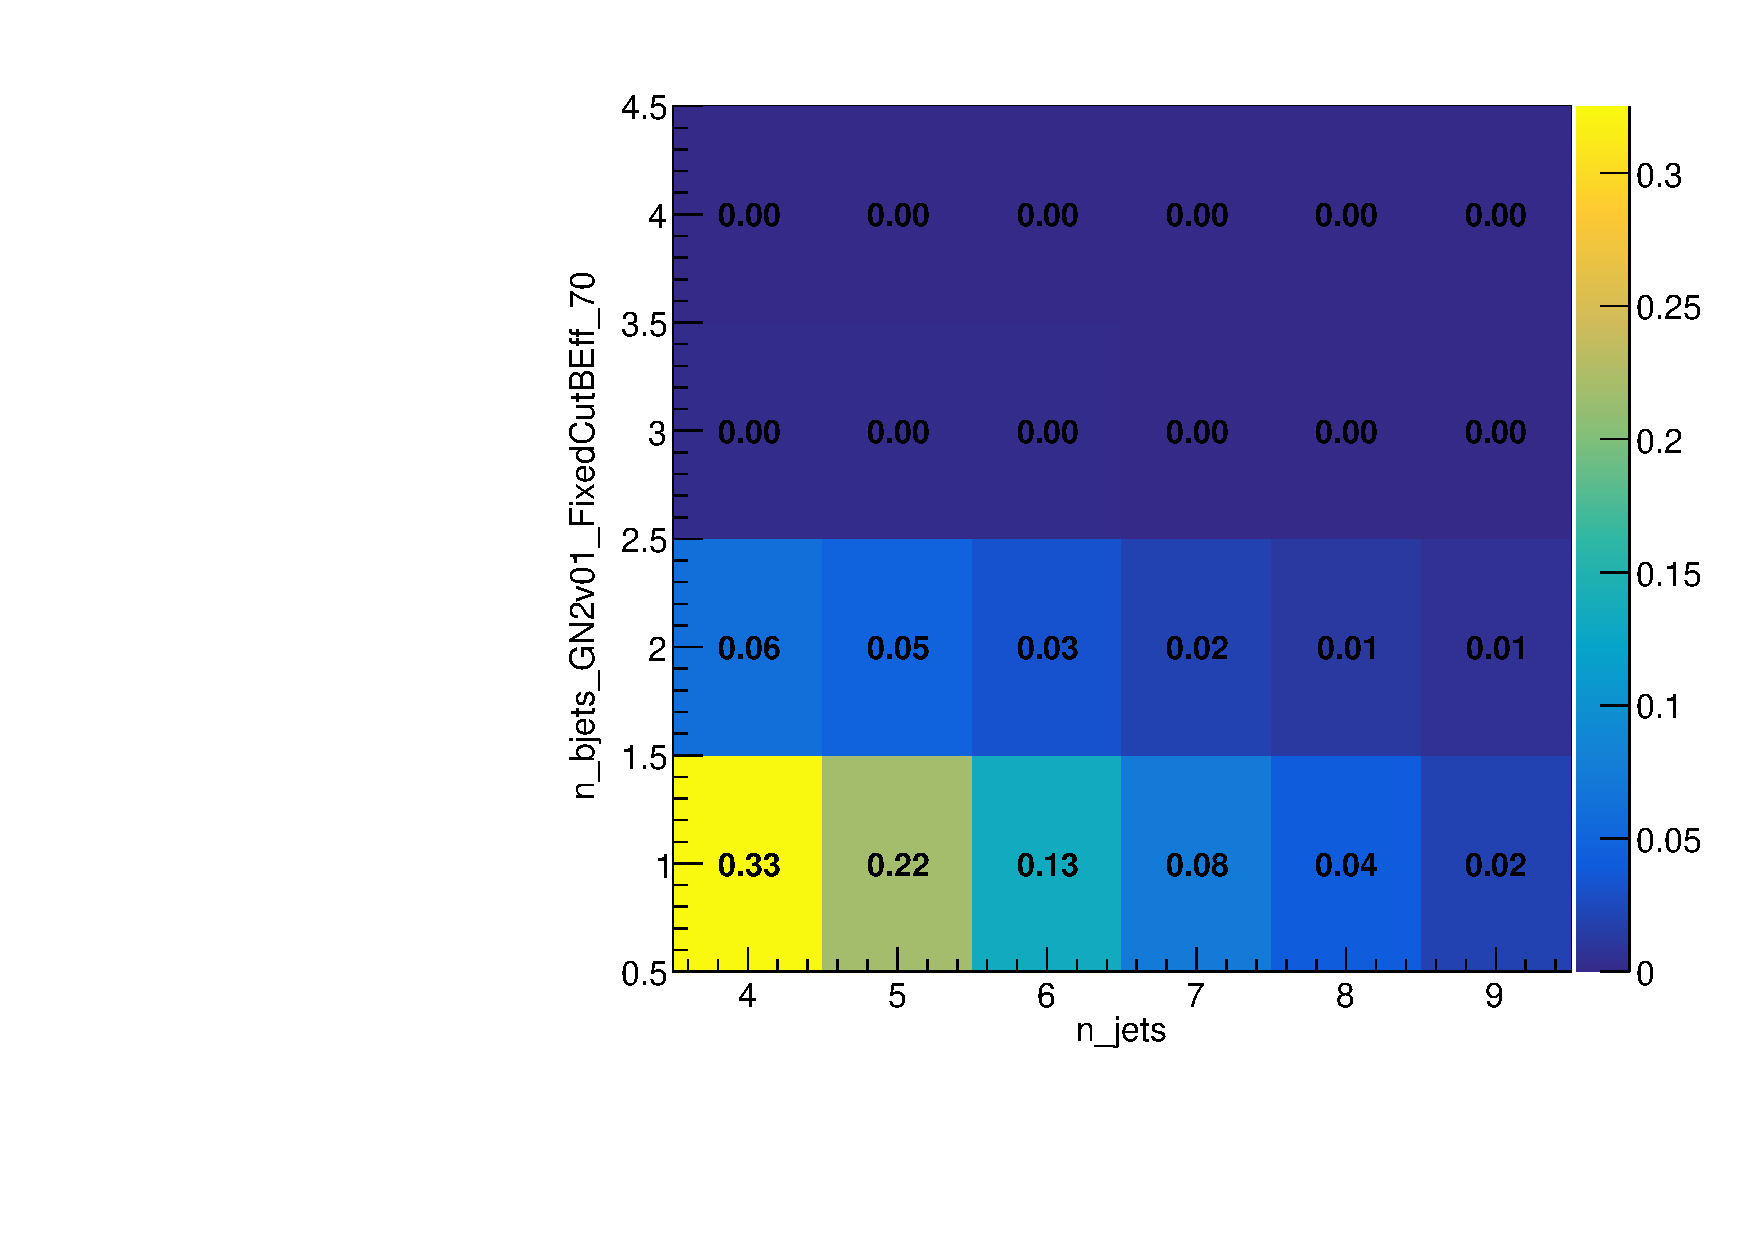
\includegraphics[width=\textwidth]{jets_selection/map_Z_frac}
      \caption{$Z\to\tau\tau$}
      \label{fig:jetsel_ztt}
    \end{subfigure}
    \hfill
    \begin{subfigure}[b]{0.48\textwidth}
      \centering
      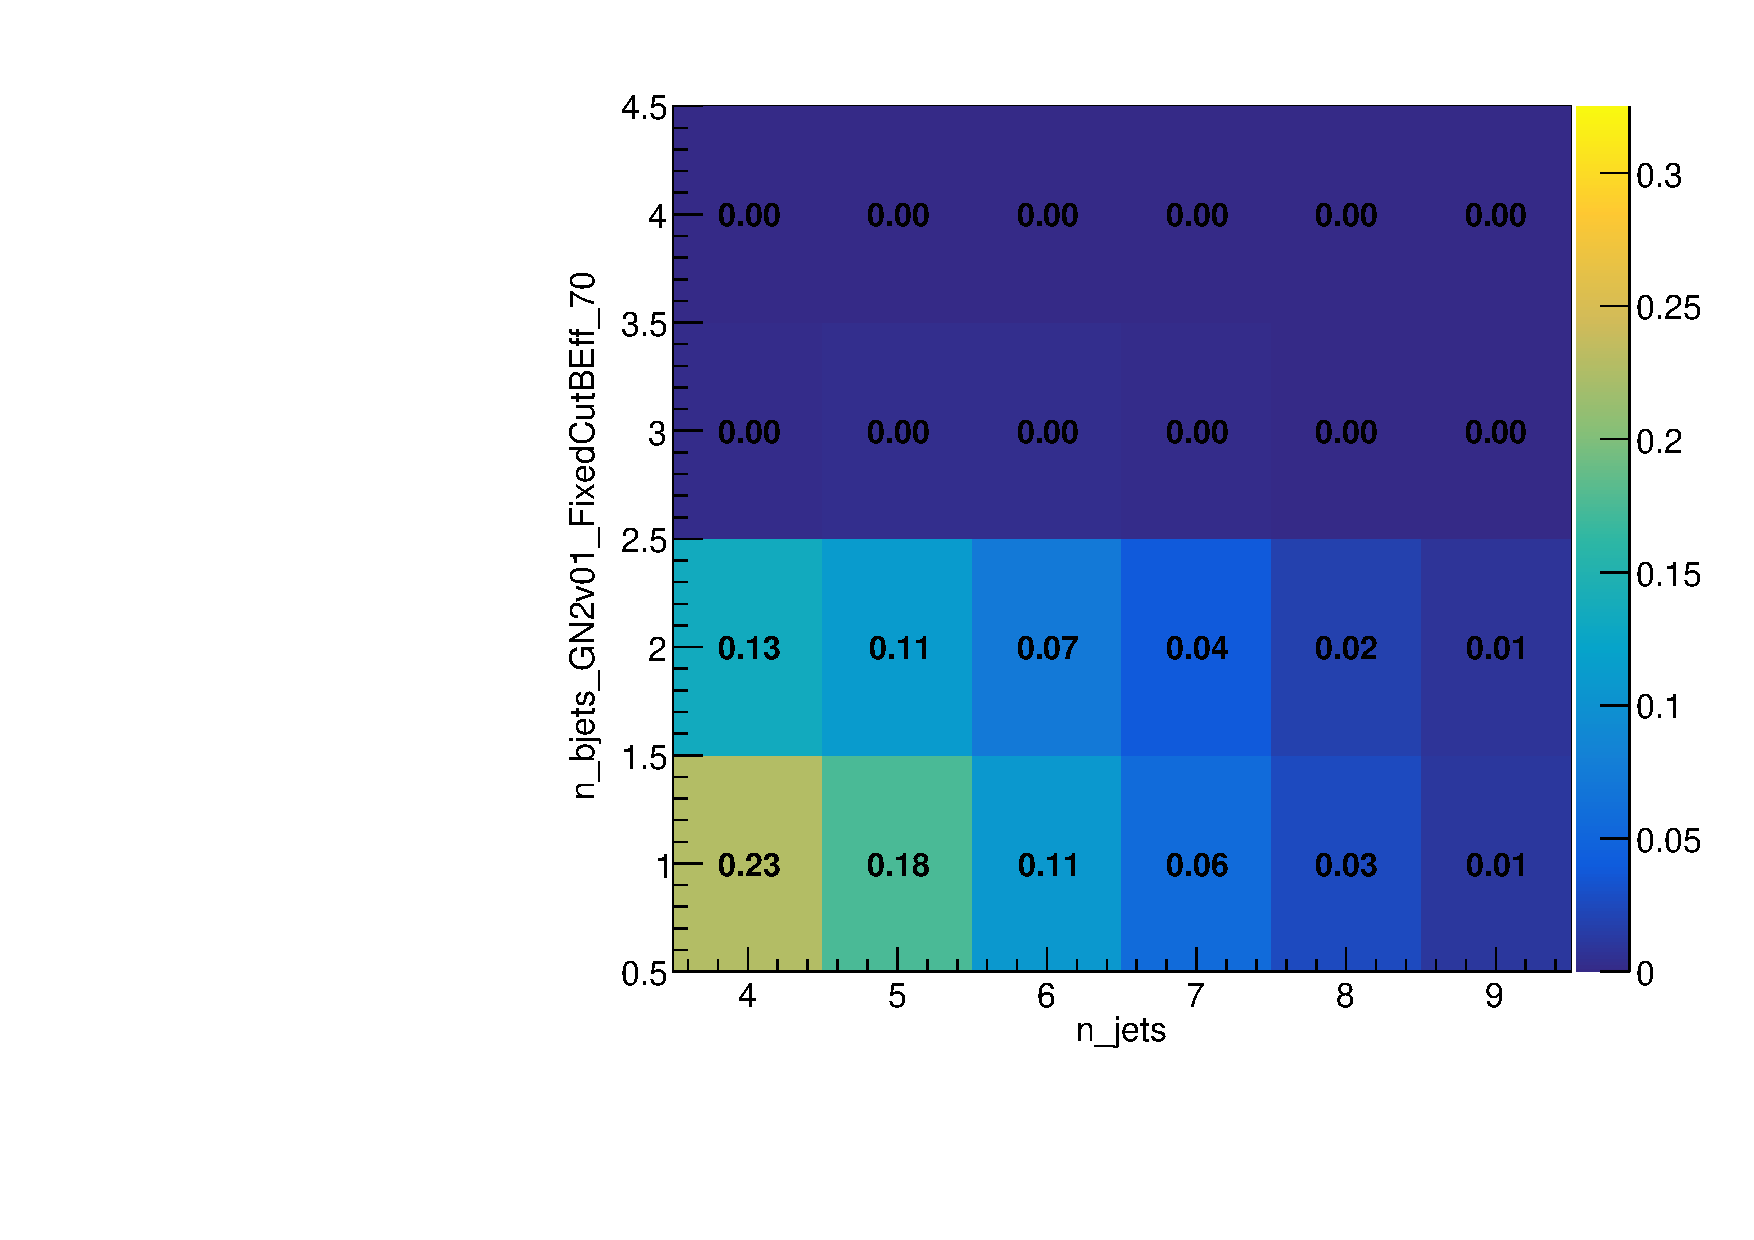
\includegraphics[width=\textwidth]{jets_selection/map_ttbar_frac}
      \caption{$t\bar{t}$}
      \label{fig:jetsel_ttbar}
    \end{subfigure}
    \\[0.3cm]
    \begin{subfigure}[b]{0.48\textwidth}
      \centering
      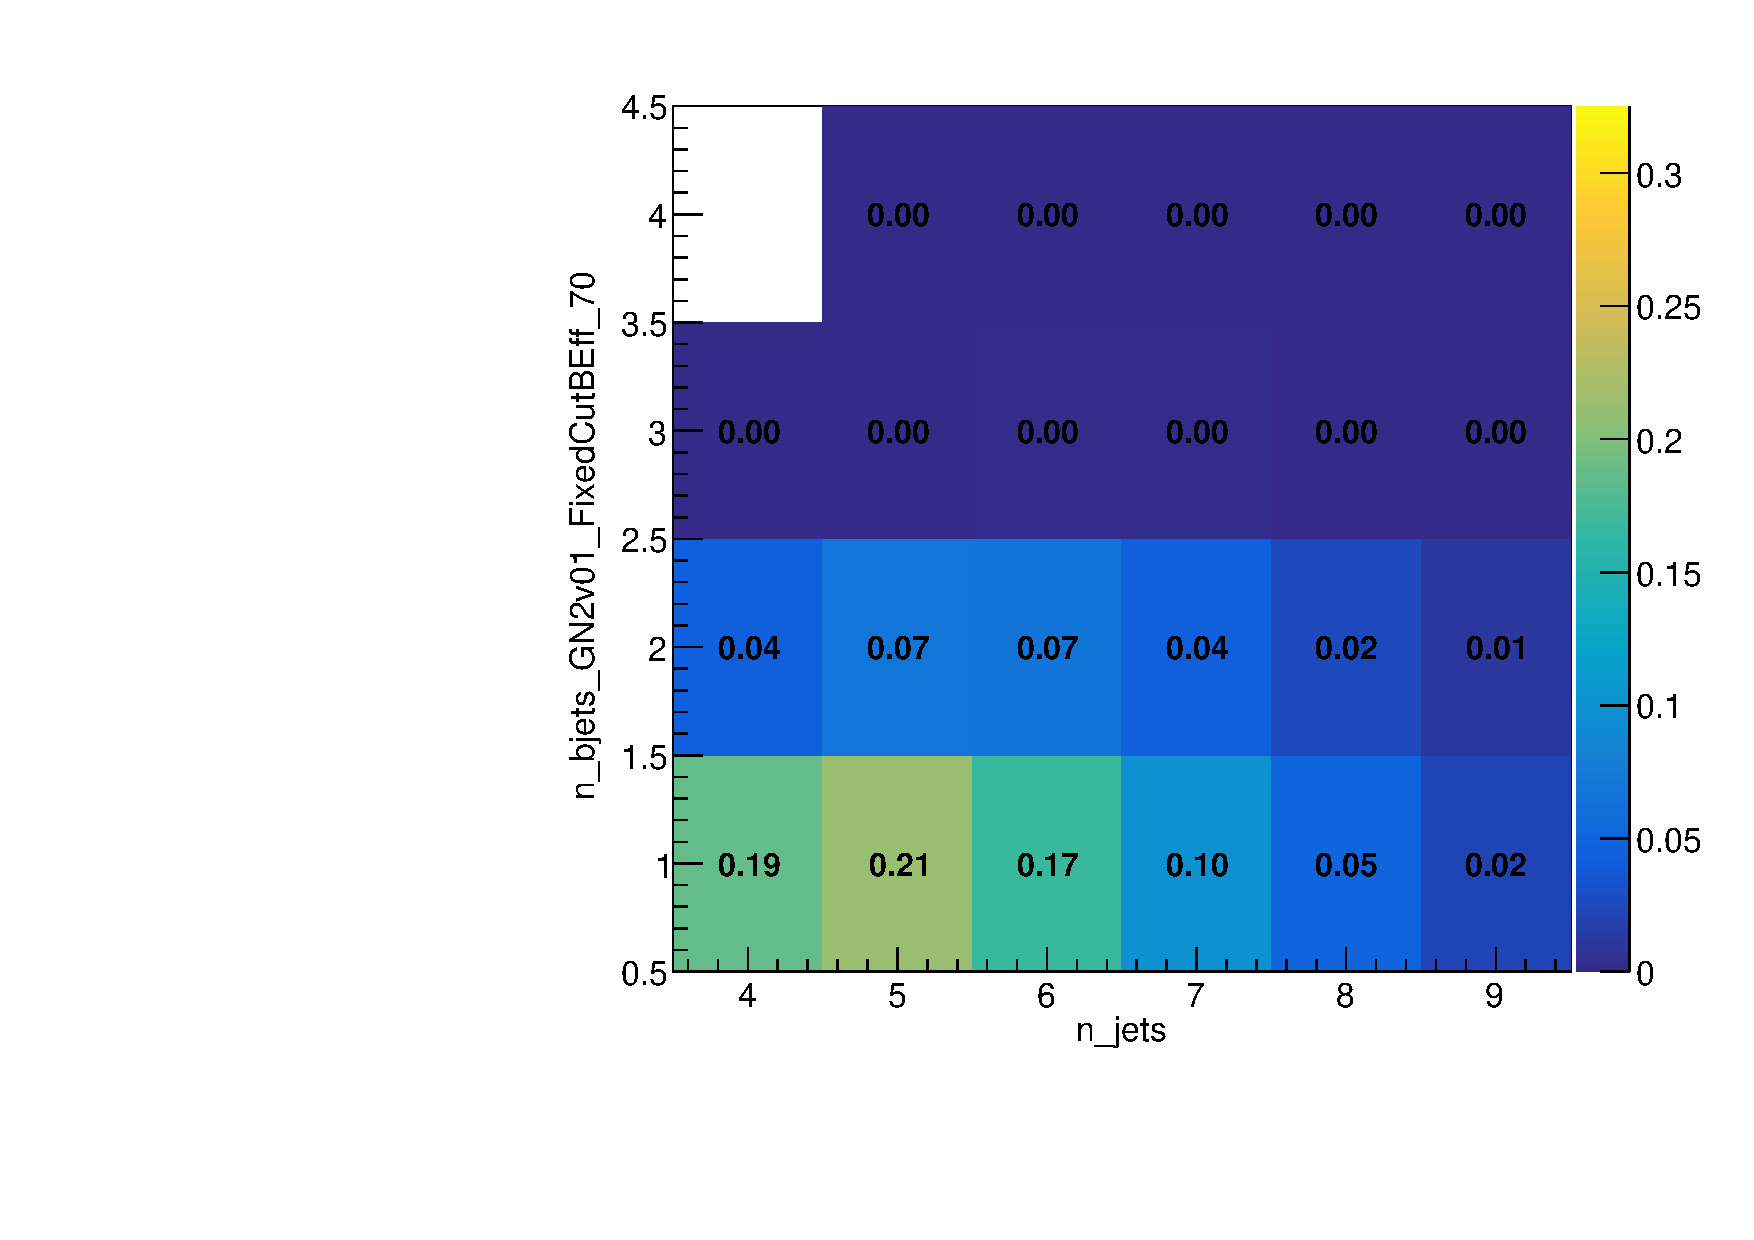
\includegraphics[width=\textwidth]{jets_selection/map_tHqb_frac}
      \caption{$tHqb$}
      \label{fig:jetsel_th}
    \end{subfigure}
    \hfill
    \begin{subfigure}[b]{0.48\textwidth}
      \centering
      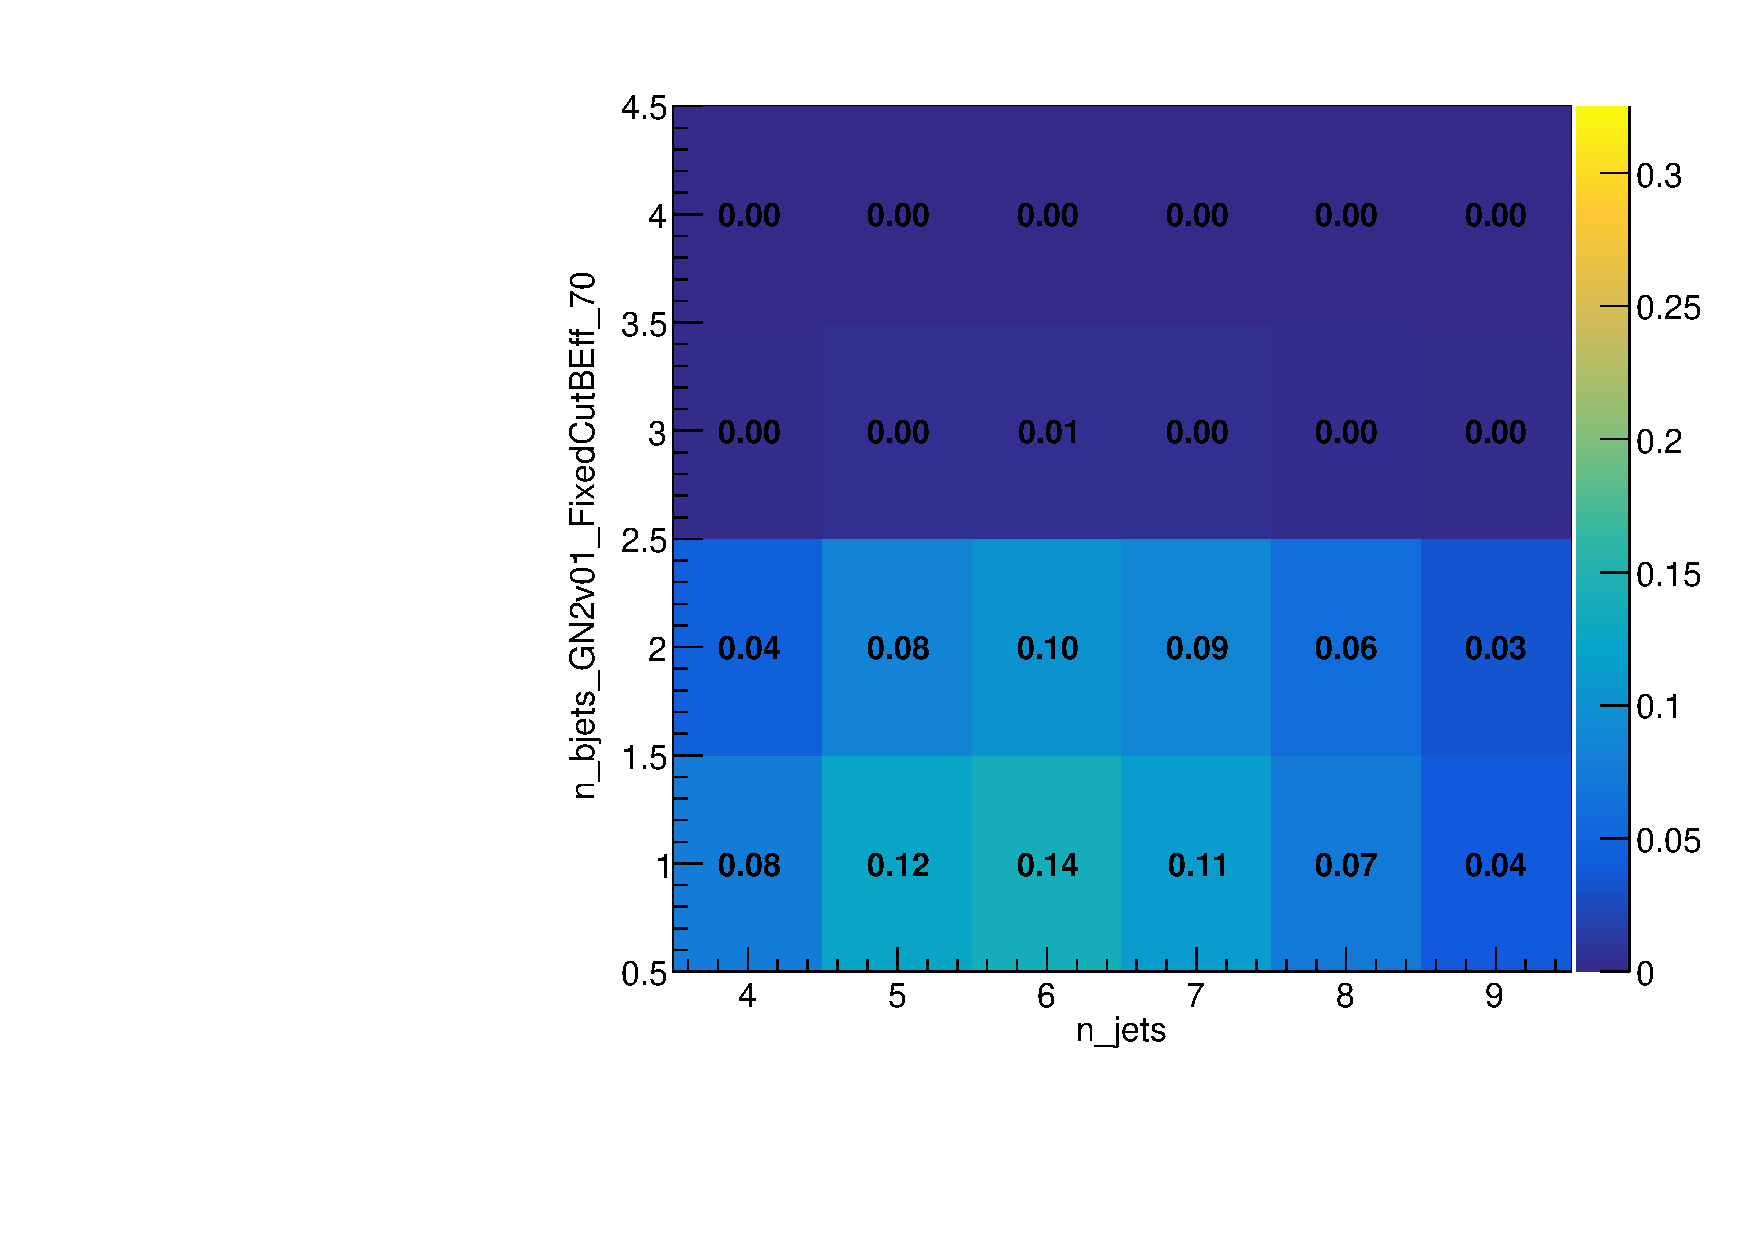
\includegraphics[width=\textwidth]{jets_selection/map_ttH_frac}
      \caption{$t\bar{t}H$}
      \label{fig:jetsel_tth}
    \end{subfigure}
    \caption{
      Fraction of events passing different requirements on the jet and $b$-jet multiplicities
      for the main signal and background processes. 
      The heatmaps show the fraction of selected events for the different processes, 
      as a function of the number of reconstructed jets and the number of $b$-tagged jets.
    }
    \label{jets_selection}
  \end{figure}
  
\section{Misidentified-$\tau$ background estimation}
\label{fakes_run3}

When estimating the contribution from fake-\tauhad backgrounds in the previous analysis the dedicated CRs were derived by inverting the identification criteria applied to the \tauhad candidates in the SRs. From these CRs, templates enriched in fake-\tauhad objects were obtained and subsequently used both to derive the fake factors (FFs) and to apply them in the analysis signal regions. An important detail was that one could not simply invert the Medium working point: at least one of the $\tau_{\mathrm{had}}$ candidates still had to satisfy a loose identification requirement, since events without any loosely identified $\tau_{\mathrm{had}}$ were not kept in the derivations. This limitation is no longer present in the samples processed with release 22, which simplifies the estimation procedure in the current study.


\subsection{Nominal FF estimation}

In the \thqb + \ttH analysis, the fake-\tauhad background is re-estimated by defining a single CR in which the $\tau_{\mathrm{had}}$ candidates fail the Medium working point, without imposing any additional Loose requirement. A single set of fake factors, $FF_{nm}$ following Eq.~\ref{eq_fakes}, is therefore enough to describe the background contribution. 

The FFs are derived in bins of \pt and $|\eta|$ of the $\tau$-lepton, using dedicated \taulephad control regions. Separate determinations are performed for Run-2 and Run-3 data, and depending on whether the hadronic $\tau$-lepton decay is classified as 1-prong or 3-prong. Figure~\ref{fig:ff_run2_run3} shows the resulting FFs for both data-taking periods, displayed as a function of \pt in the two $|\eta|$ regions considered: the ``Barrel'' region ($0<|\eta|<1.37$) and the ``Endcap'' region, which covers the remaining acceptance.
\begin{figure}[htbp]
    \centering
    \begin{subfigure}[b]{0.49\textwidth}
      \centering
      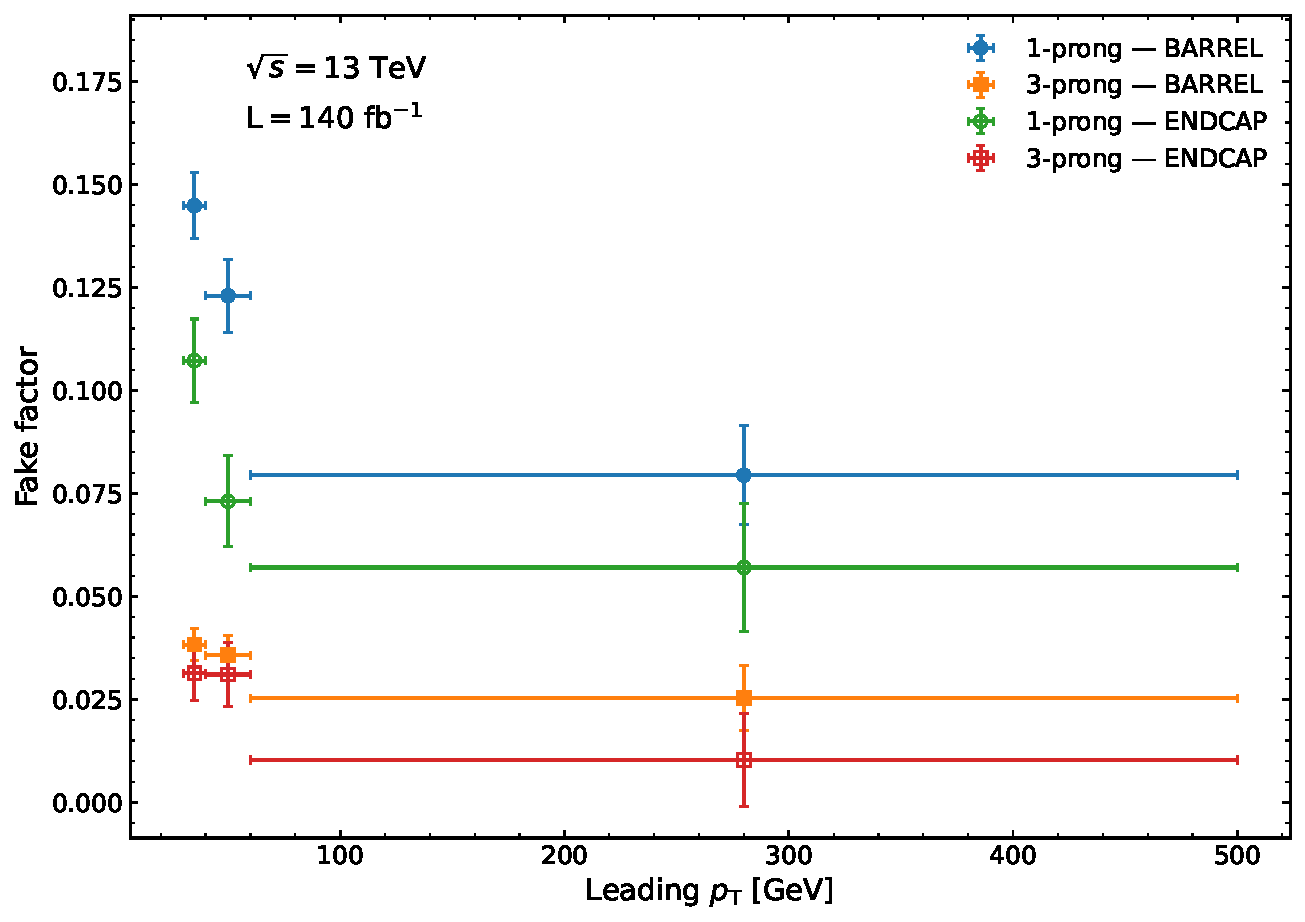
\includegraphics[width=\textwidth]{new_FFs_trigger_corrected_ATLAS_run2.pdf}
      \caption{Run~2}
      \label{fig:ff_run2}
    \end{subfigure}
    \hfill
    \begin{subfigure}[b]{0.49\textwidth}
      \centering
      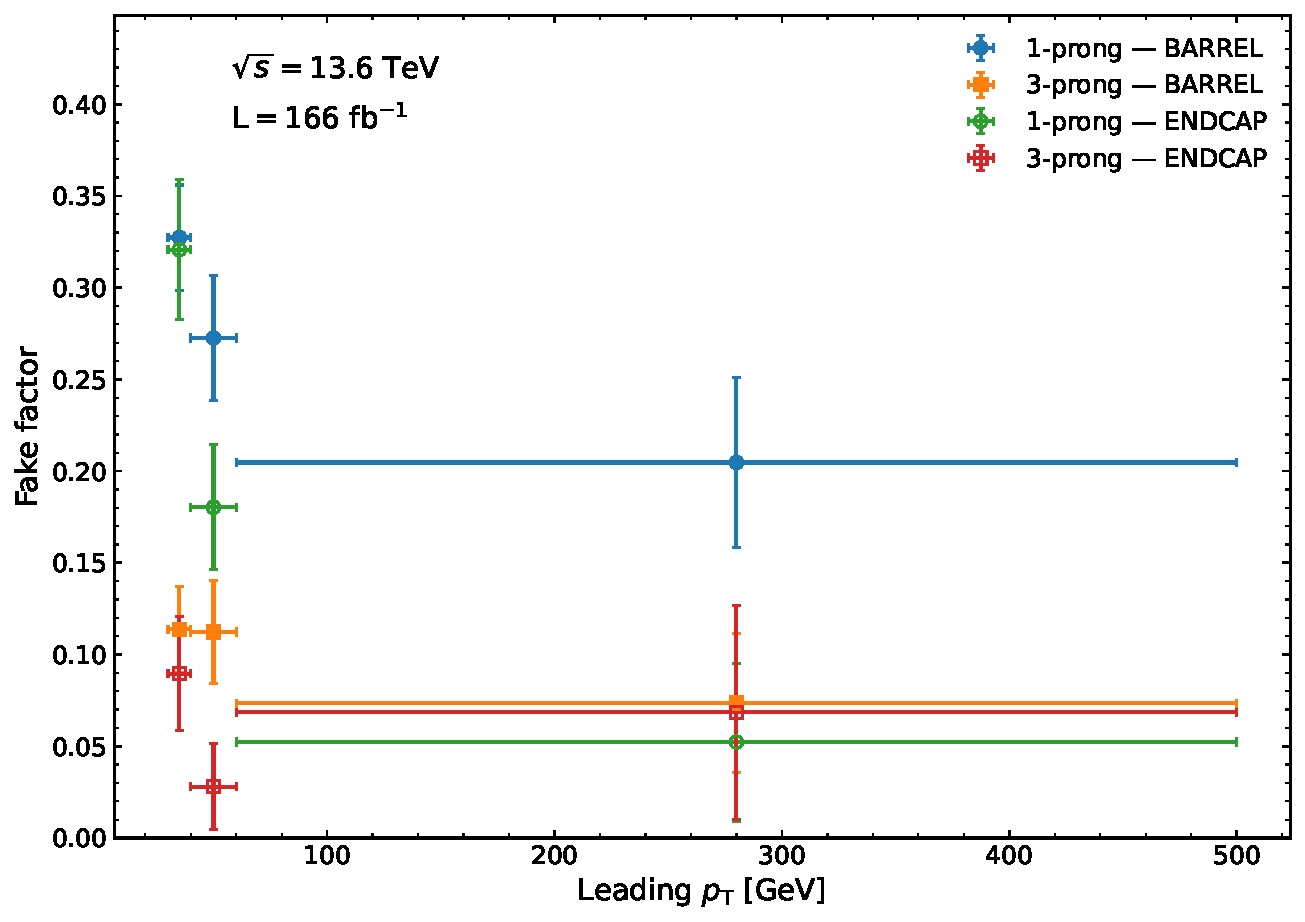
\includegraphics[width=\textwidth]{new_FFs_trigger_corrected_ATLAS_run3.pdf}
      \caption{Run~3}
      \label{fig:ff_run3}
    \end{subfigure}
    \caption{
      FFs in the \tauhadhad channel as a function of the leading $p_{\mathrm{T}}$,
      shown separately for barrel and endcap and for 1-prong and 3-prong candidates. Only statistical uncertainties are included.
    }
    \label{fig:ff_run2_run3}
  \end{figure}
From these plots it can be concluded that the FFs required to scale the background from misidentified \tauhad are significantly larger for Run-3 data compared to Run-2, particularly at low \pt, with the effect being especially pronounced in the 1-prong category. 
  \begin{figure}[htbp]
    \centering
    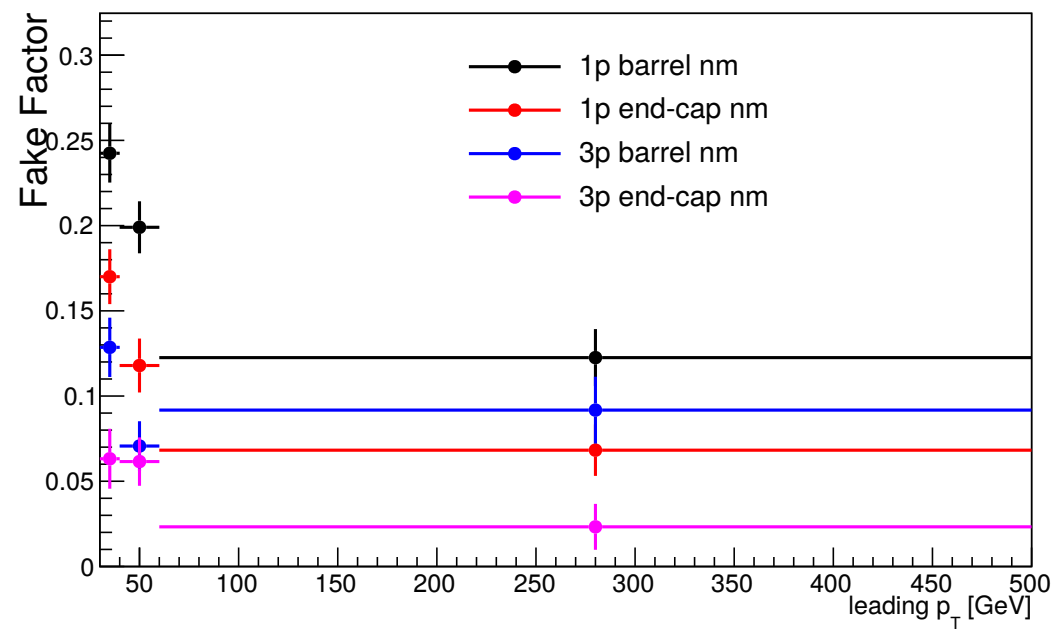
\includegraphics[width=0.55\textwidth]{ffs_run2_legacy}
    \caption{FFs derived in Run-2 using the RNN-based \tauhad identification, 
    shown as a function of the $\tau$-lepton transverse momentum for the same two $|\eta|$ regions considered: Barrel and Endcap~\cite{serhat_tesis}.}
    \label{fig:ffs_run2_rnn}
  \end{figure}

More importantly, the new FFs derived with release~22 Run-2 samples using the updated \textsc{gntau} identification algorithm are noticeably smaller than those obtained in the previous round of the analysis presented in the preceding chapter, which relied on the RNN-based approach for \tauhad identification~\cite{serhat_tesis}, as illustrated in Figure~\ref{fig:ffs_run2_rnn}.  
This difference is observed across all \pt and $|\eta|$ bins, both for 1- and 3-prong. At first sight, it could suggest that the new \textsc{gntau} algorithm achieves a better performance in rejecting jets faking \tauhad. In the following, the closure or validation of this new fake-\tauhad background estimate is presented, together with a comparison to the results obtained in the previous round, in order to quantify the extent to which this background has been reduced.

In this simplified scenario, the application of the FFs follows a straightforward event-by-event reweighting: events in which only one $\tau_{\mathrm{had}}$ candidate fails the Medium ID are scaled by the $FF_{nm}$ of the failing $\tau$, while events where both candidates fail are scaled by the negative product of the two FFs, in order to prevent double-counting. The full prediction in the signal region is thus given by
\begin{align}
    \tau_1^{P}\,\tau_2^{P} \;=\;&\;
    \tau_1^{T}\,\tau_2^{T}\;(\text{MC}) \nonumber \\[0.2cm]
    &+\, FF_{nm}(\tau_1)\;\tau_1^{F}\,\tau_2^{P} \nonumber \\[0.2cm]
    &+\, FF_{nm}(\tau_2)\;\tau_1^{P}\,\tau_2^{F} \nonumber \\[0.2cm]
    &-\, FF_{nm}(\tau_1)\,FF_{nm}(\tau_2)\;\tau_1^{F}\,\tau_2^{F}\,,
    \label{eq_fakes}
    \end{align}
where $P$ and $F$ denote whether a $\tau_{\mathrm{had}}$ candidate passes or fails the Medium ID, respectively, and $\tau^T$ refers to genuine $\tau$-leptons taken from simulation in order to estimate the contribution from genuine \tauhad in the SR.  
To validate the estimation of this background contribution, the distributions of representative observables such as the transverse momentum and pseudorapidity of the leading and subleading \tauhad candidates are shown in Figures~\ref{fig:closure_validation_run2} and~\ref{fig:closure_validation_run3} at preselection level, inclusive in jet multiplicity to allow for a clearer visualization.  
These plots are evaluated in a same-sign region, which is enriched in events with misidentified \tauhad candidates. In these events, the large jet multiplicity and the random charge assignment of tracks increase the probability of jets mimicking the signature of hadronic $\tau$ decays. Good agreement between data and the background estimation is expected. 
    
  \begin{figure}[htbp]
    \centering
    \begin{subfigure}[b]{0.45\textwidth}
      \centering
      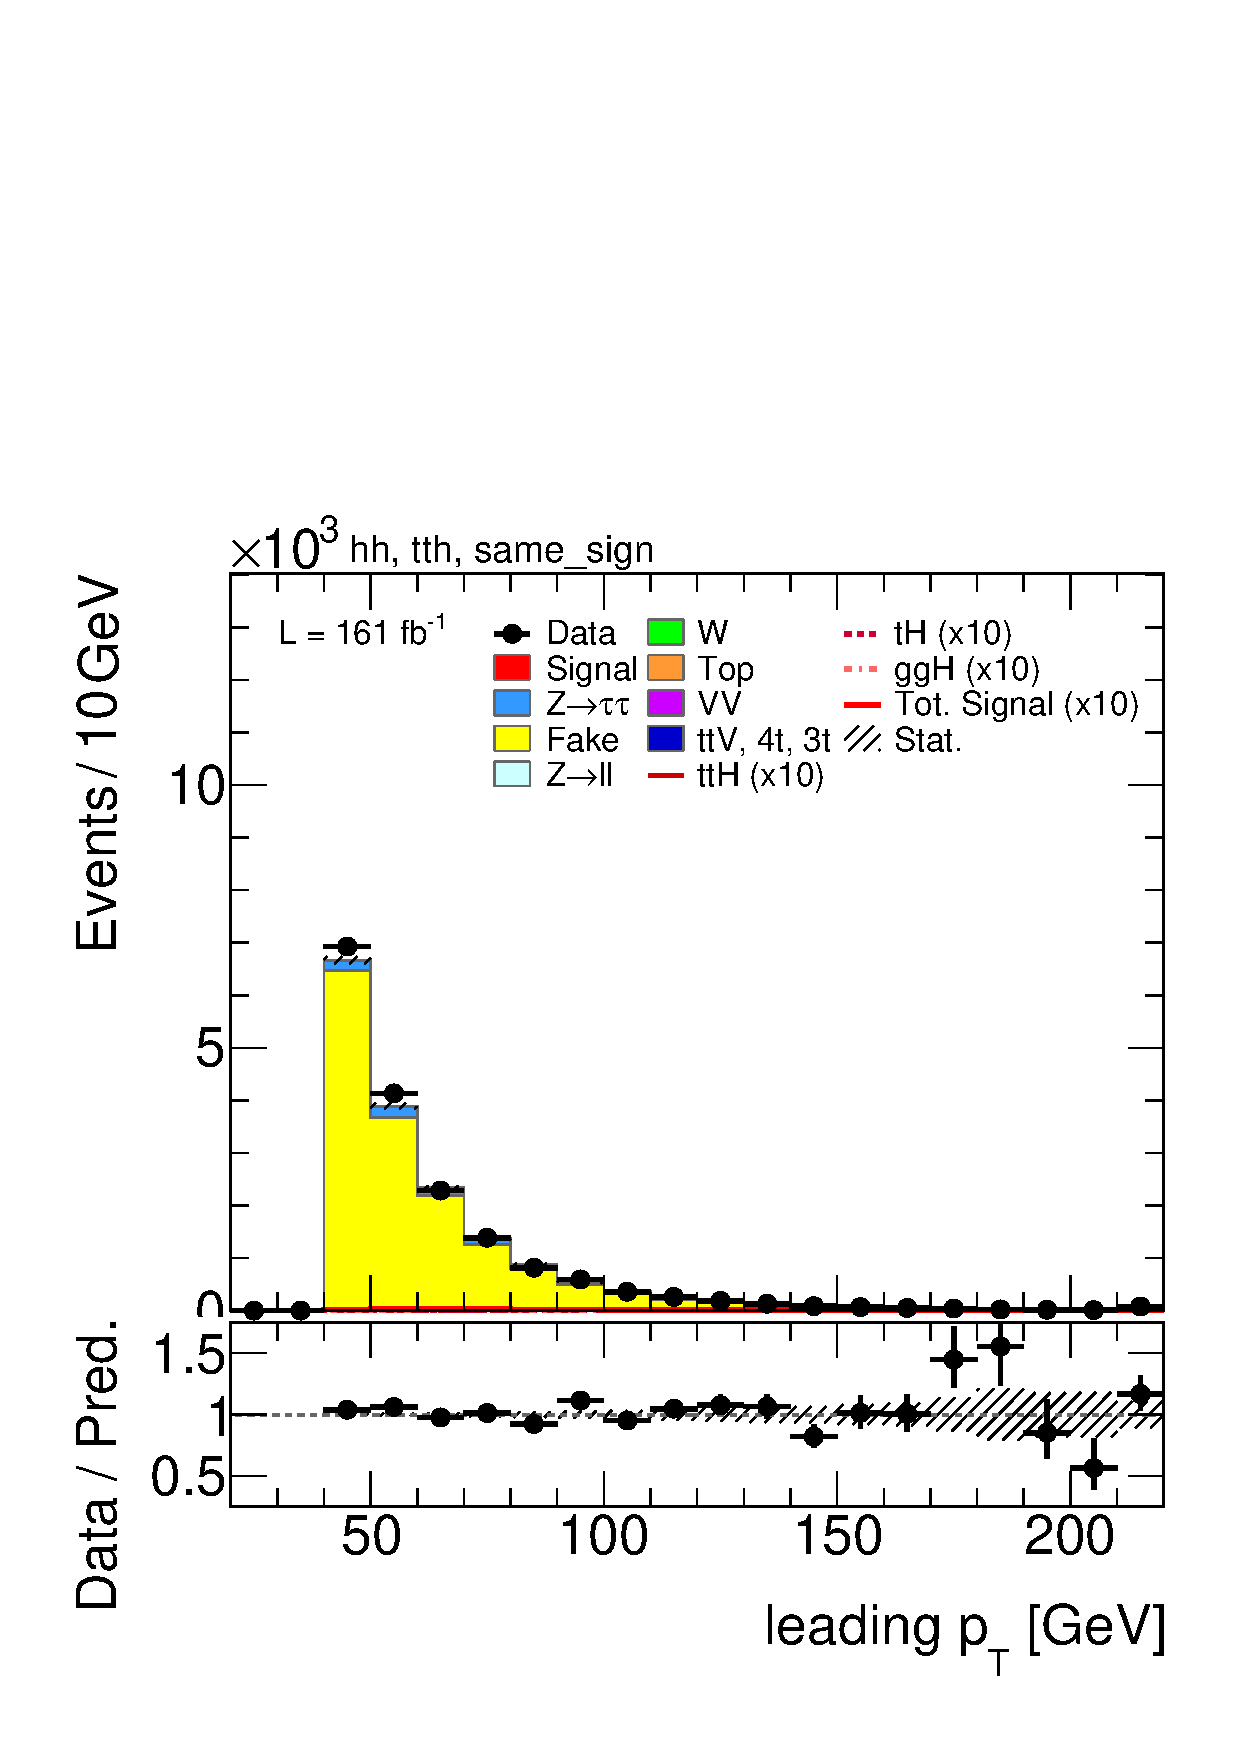
\includegraphics[width=\textwidth]{images/fakes_run3/plot_tau_0_pt_hh_tth_22_23_24_same_sign.pdf}
      \caption{}
    \end{subfigure}
    \hfill
    \begin{subfigure}[b]{0.45\textwidth}
      \centering
      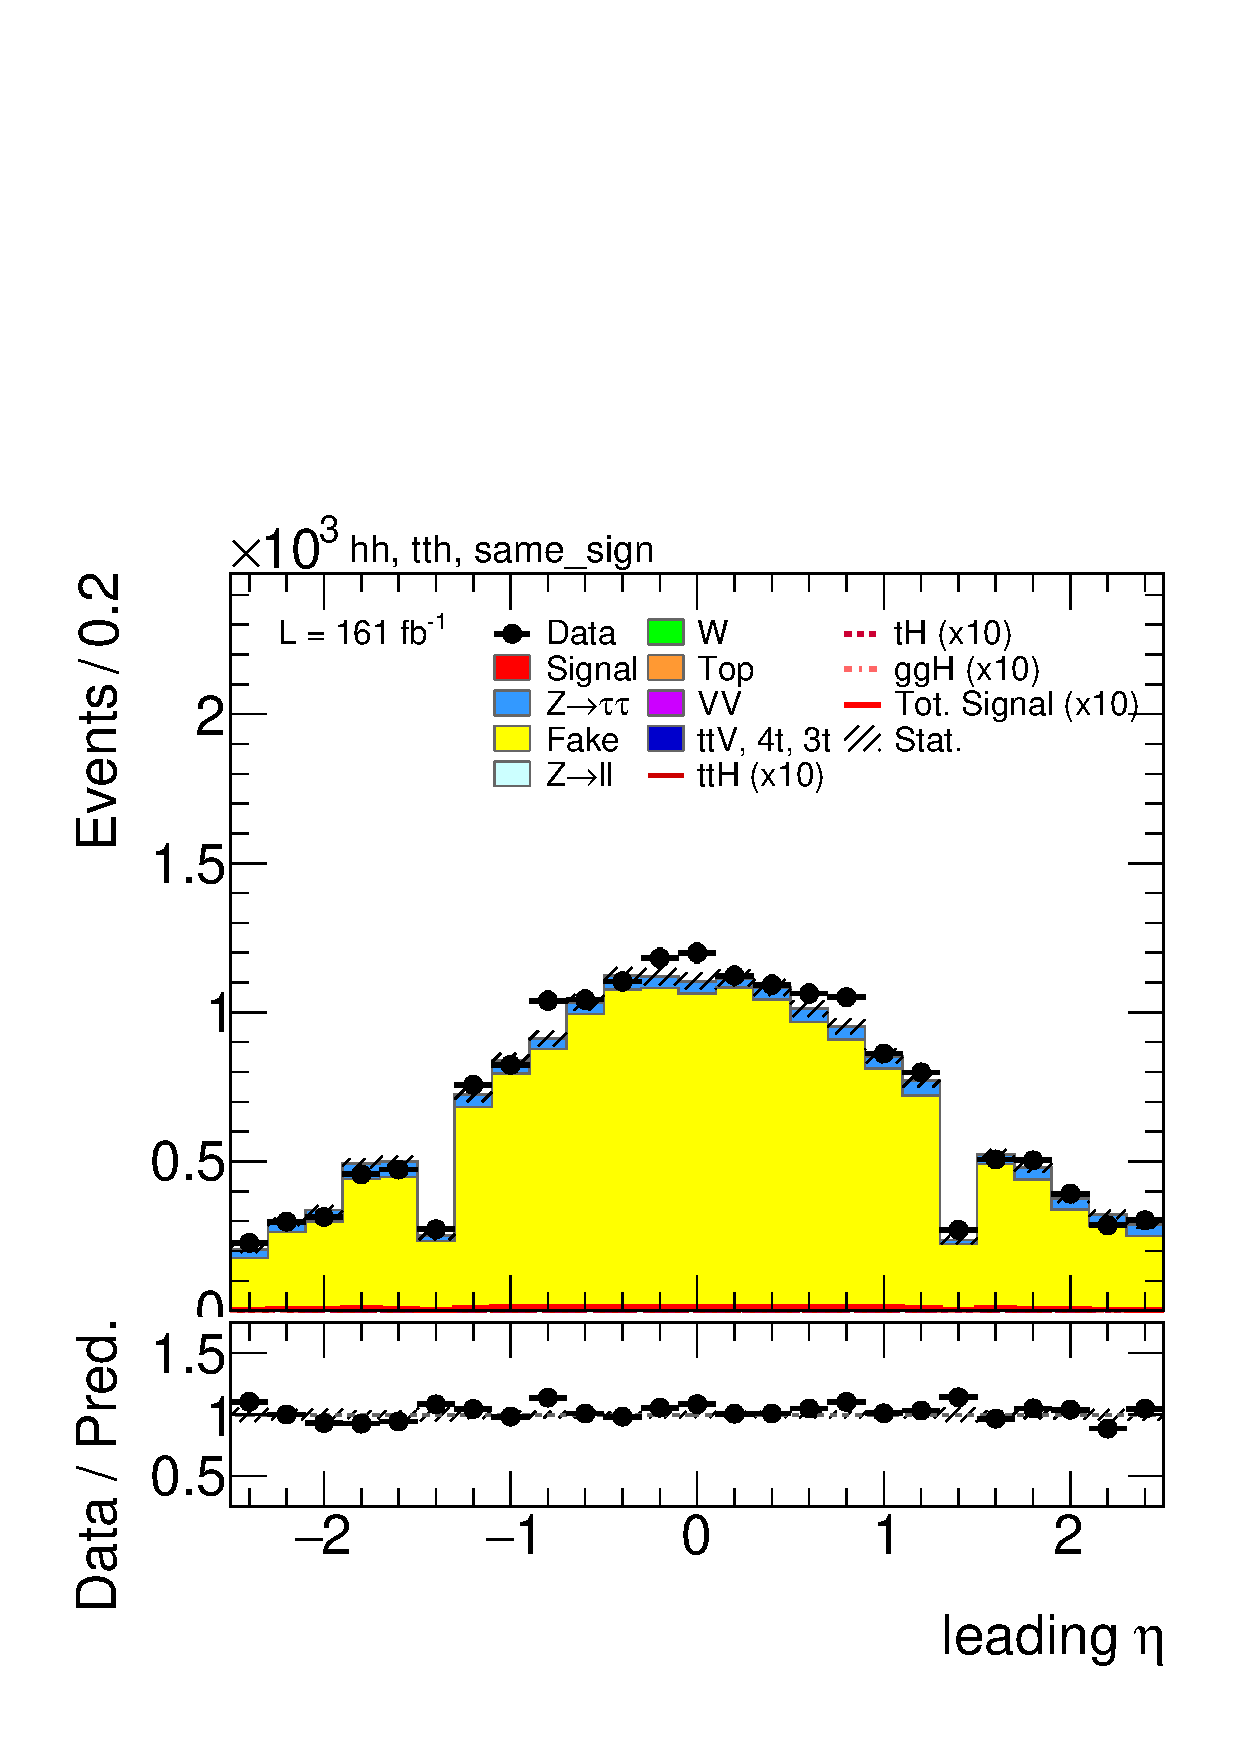
\includegraphics[width=\textwidth]{images/fakes_run3/plot_tau_0_eta_hh_tth_22_23_24_same_sign.pdf}
      \caption{}
    \end{subfigure}

    \begin{subfigure}[b]{0.45\textwidth}
      \centering
      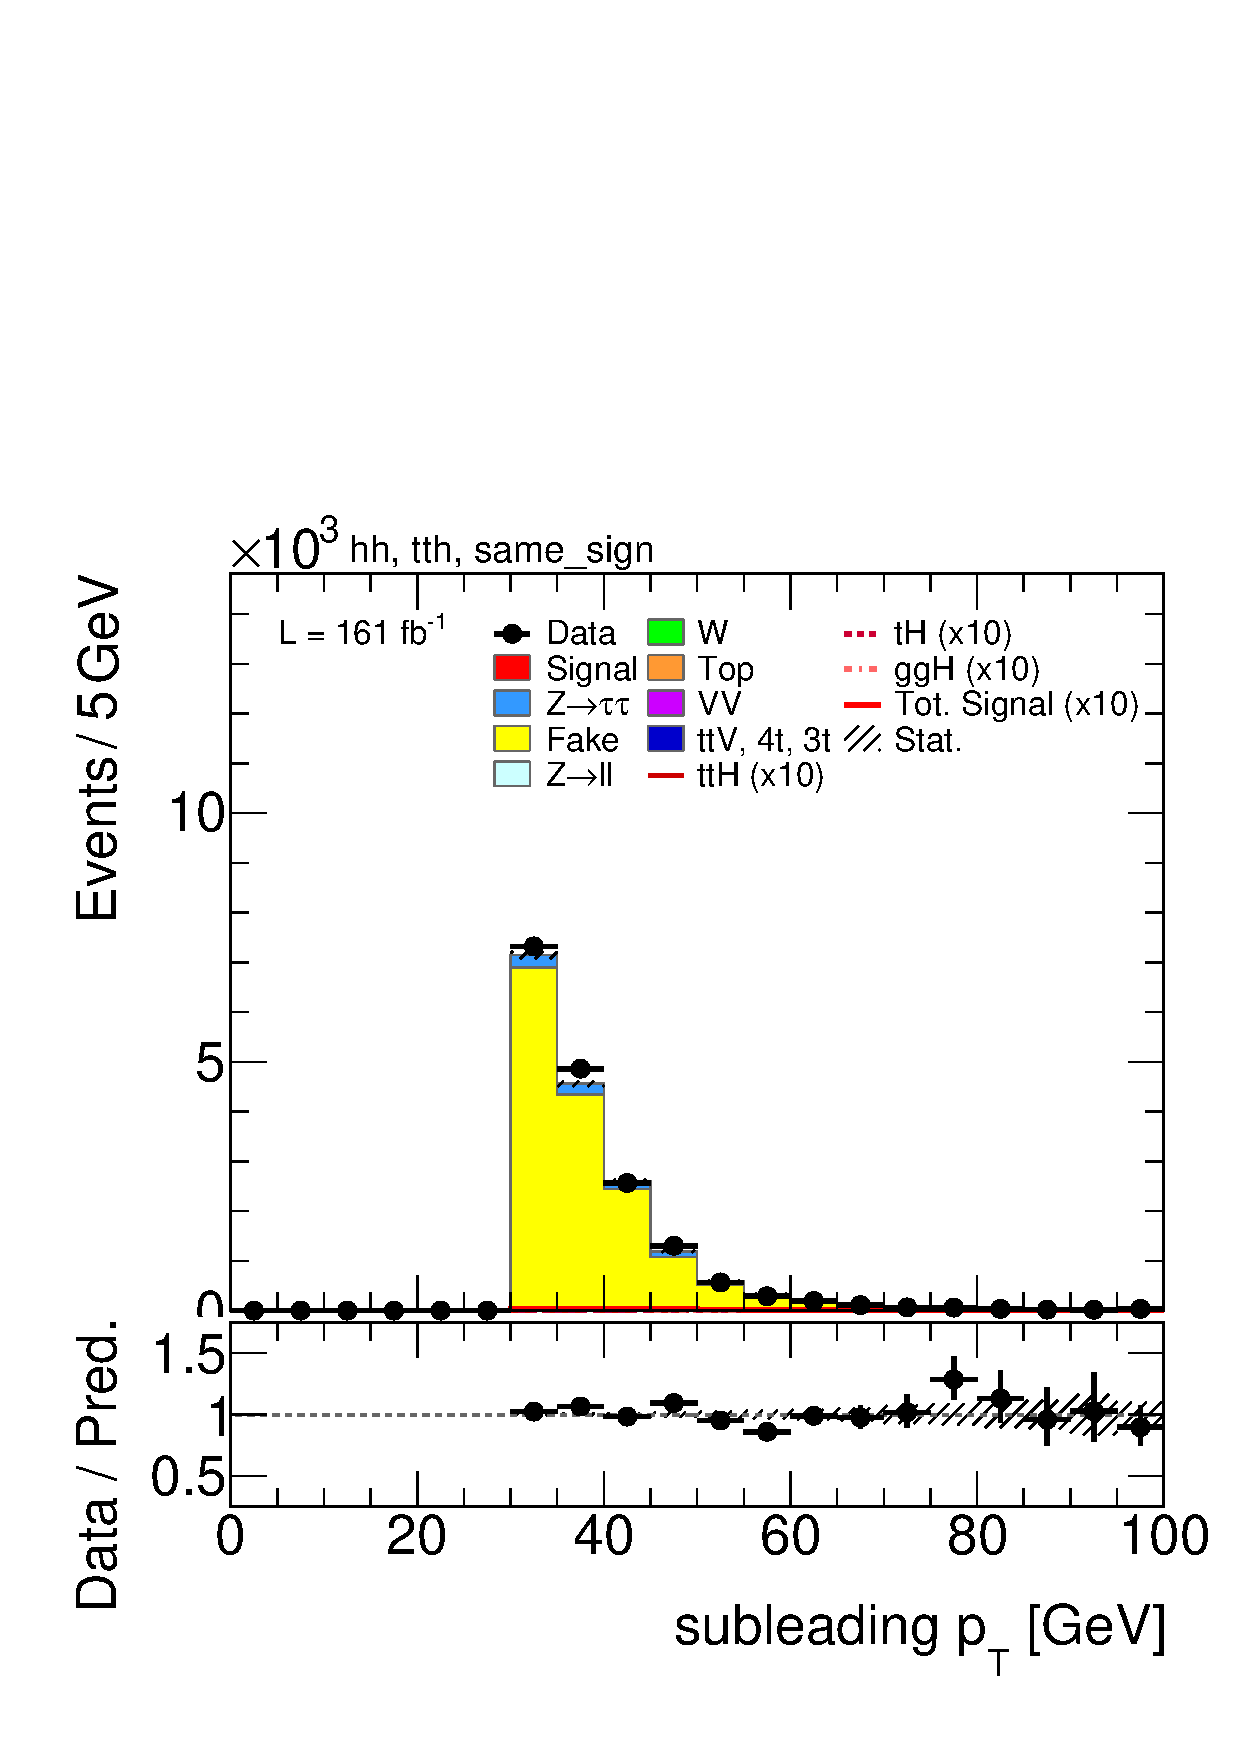
\includegraphics[width=\textwidth]{images/fakes_run3/plot_tau_1_pt_hh_tth_22_23_24_same_sign.pdf}
      \caption{}
    \end{subfigure}
    \hfill
    \begin{subfigure}[b]{0.45\textwidth}
      \centering
      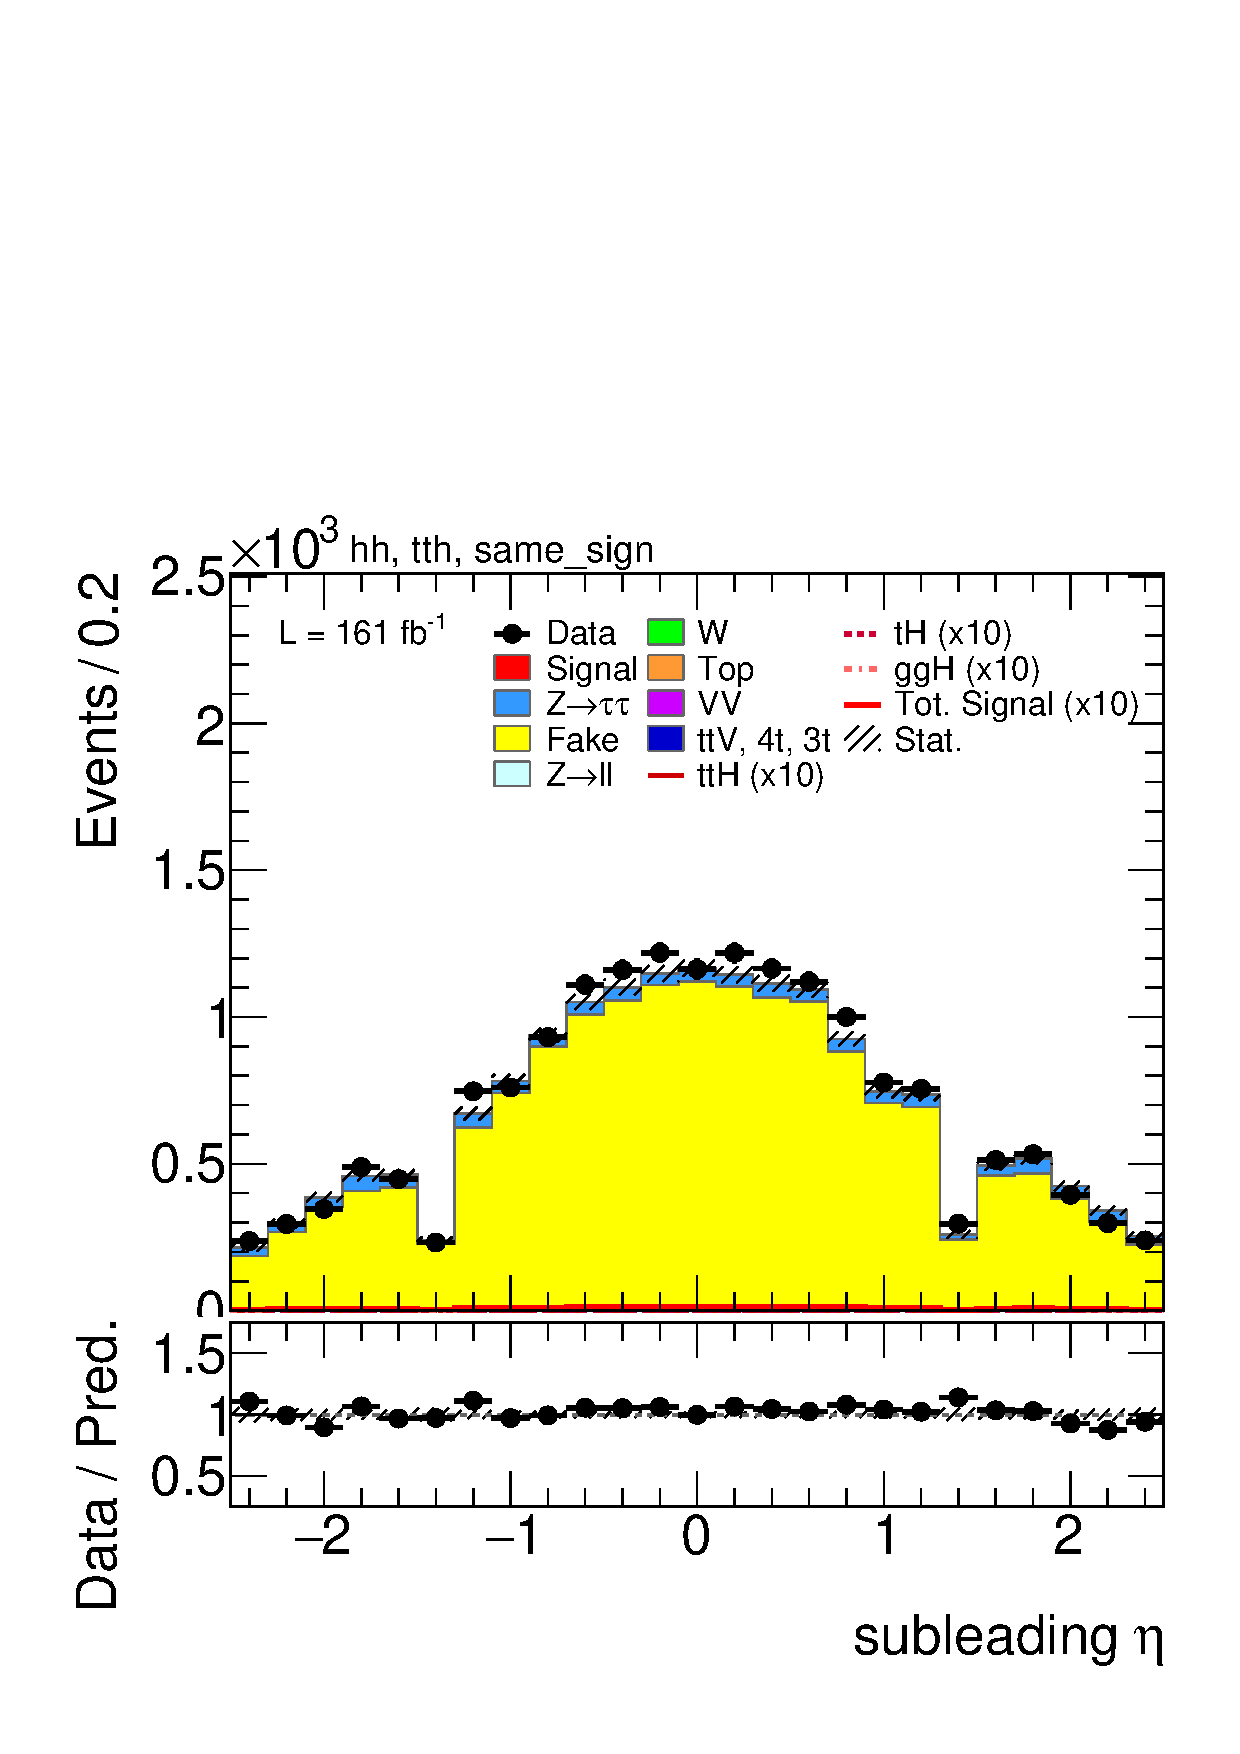
\includegraphics[width=\textwidth]{images/fakes_run3/plot_tau_1_eta_hh_tth_22_23_24_same_sign.pdf}
      \caption{}
    \end{subfigure}
  
    \caption{
      Closure and validation of the fake-\tauhad background estimation in Run-3 dataset, evaluated in the same-sign region at preselection level.
      The comparison is shown as a function of the \pt and $\eta$ of the leading (a), (b), and subleading (c), (d), \tauhad candidates. 
      Data are compared to the estimated fake-\tauhad background. Scaling factors on \ztautau and \ttbar are applied. Only statistical uncertainties are included.
    }
    \label{fig:closure_validation_run3}
  \end{figure}

  \begin{figure}[htbp]
    \centering
    \begin{subfigure}[b]{0.45\textwidth}
      \centering
      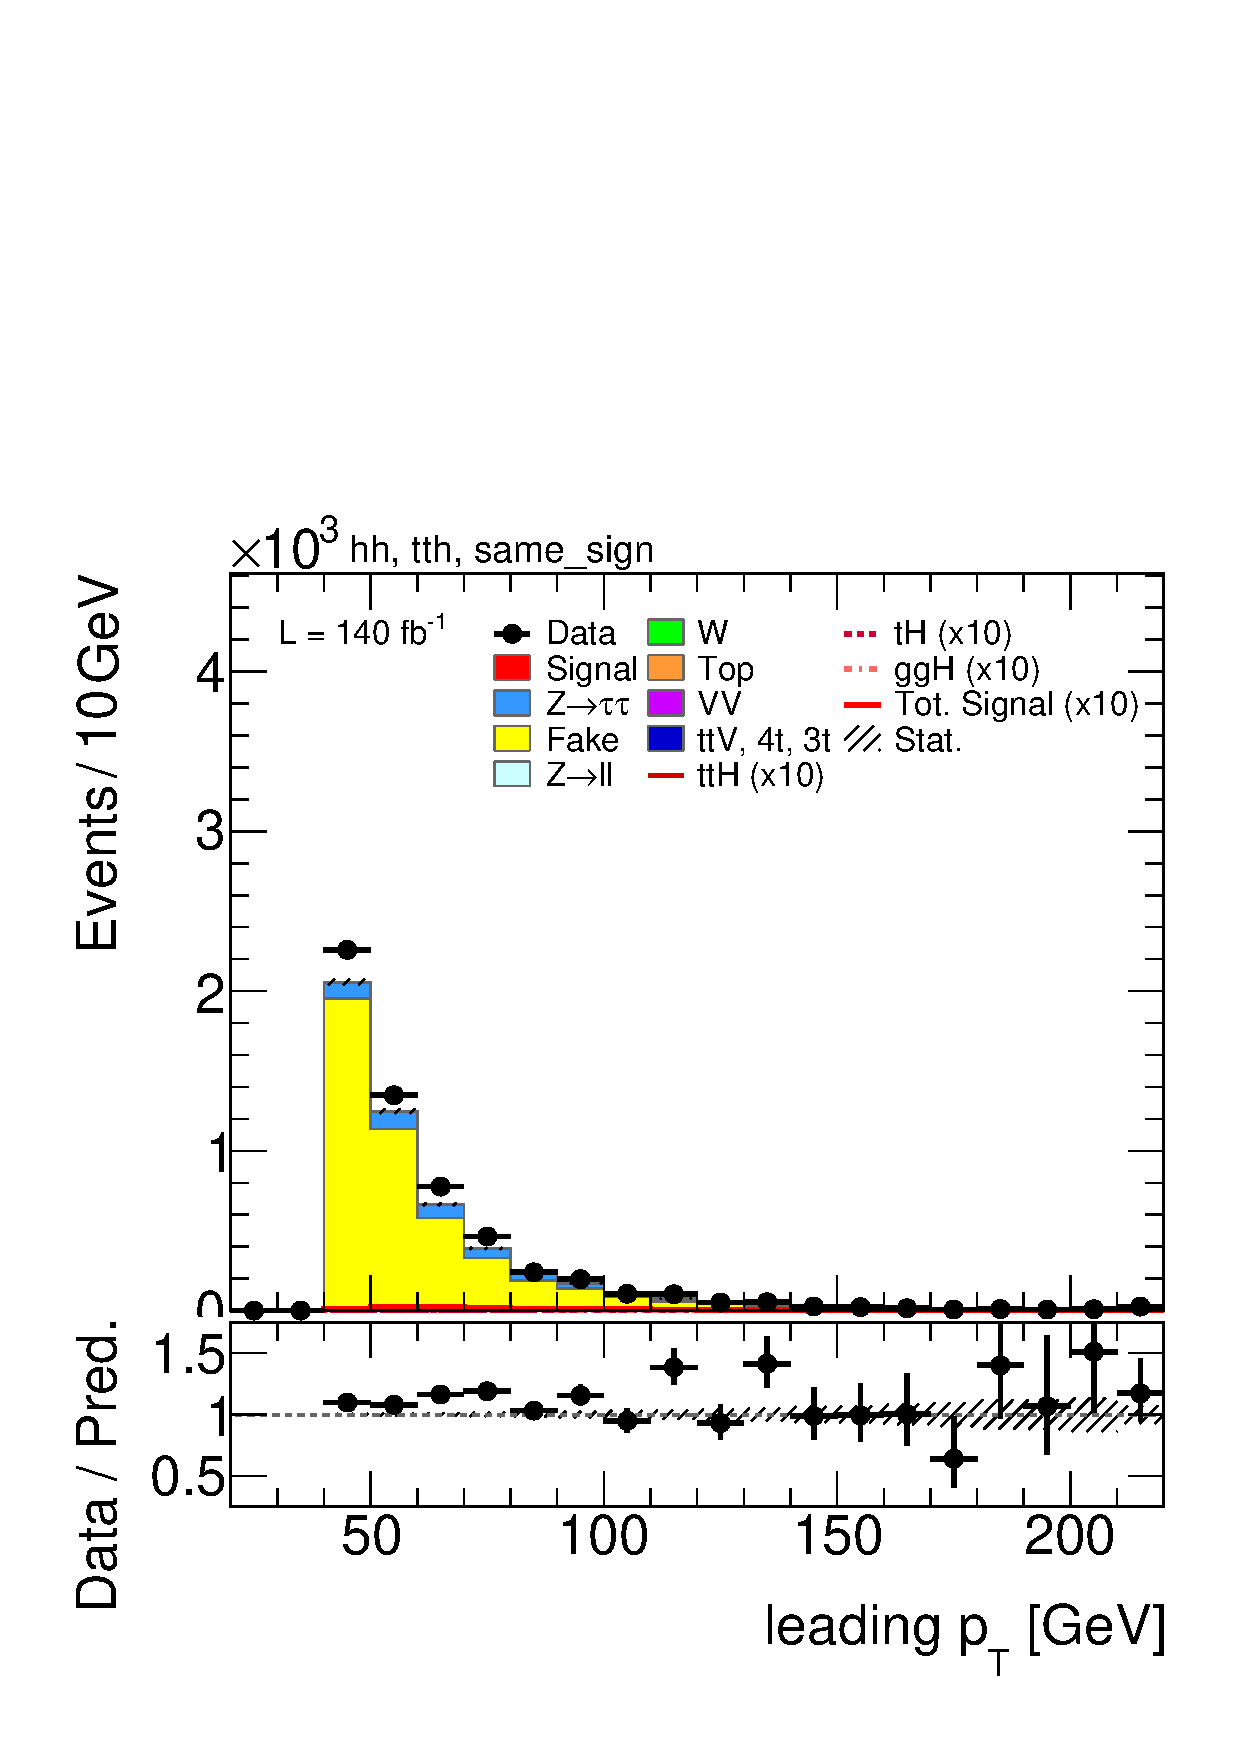
\includegraphics[width=\textwidth]{images/fakes_run2/plot_tau_0_pt_hh_tth_15_16_17_18_same_sign.pdf}
      \caption{}
    \end{subfigure}
    \hfill
    \begin{subfigure}[b]{0.45\textwidth}
      \centering
      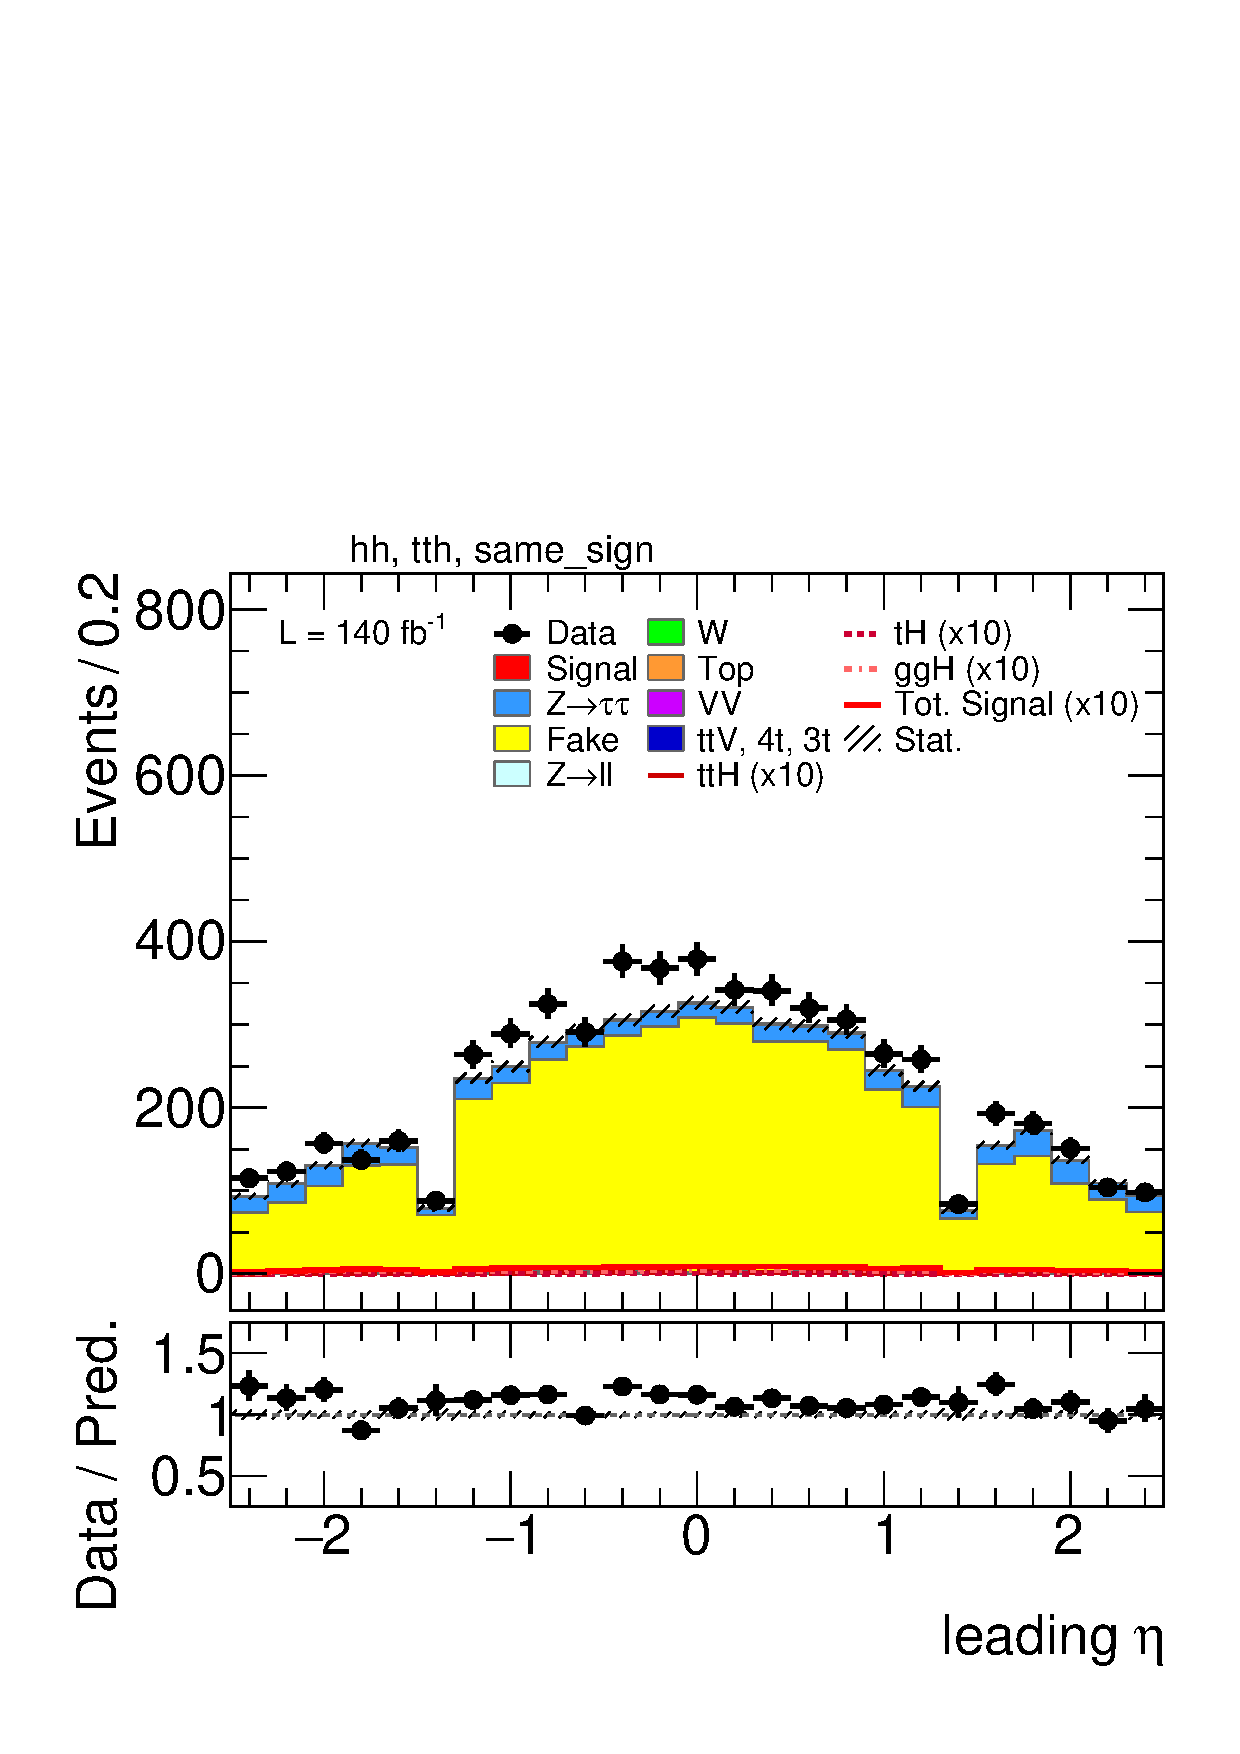
\includegraphics[width=\textwidth]{images/fakes_run2/plot_tau_0_eta_hh_tth_15_16_17_18_same_sign.pdf}
      \caption{}
    \end{subfigure}

    \begin{subfigure}[b]{0.45\textwidth}
      \centering
      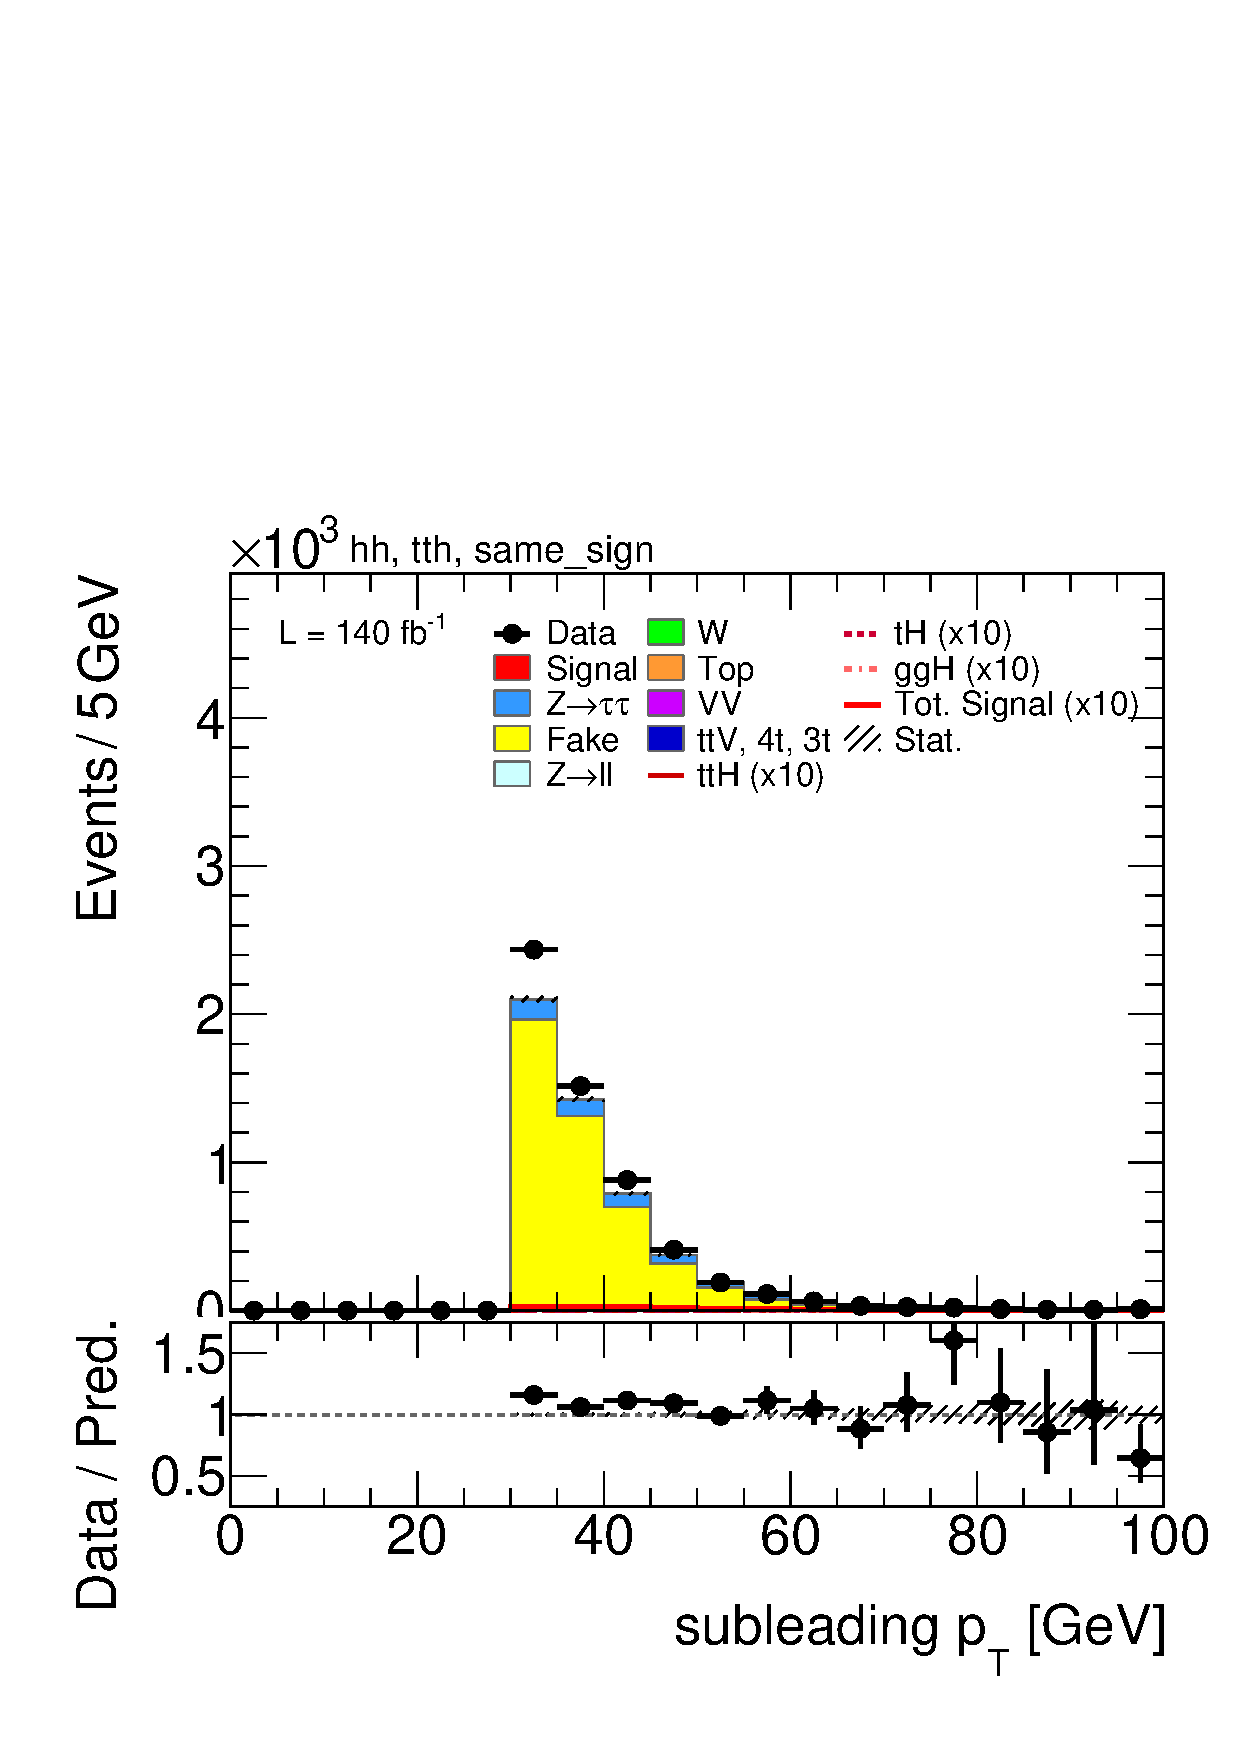
\includegraphics[width=\textwidth]{images/fakes_run2/plot_tau_1_pt_hh_tth_15_16_17_18_same_sign.pdf}
      \caption{}
    \end{subfigure}
    \hfill
    \begin{subfigure}[b]{0.45\textwidth}
      \centering
      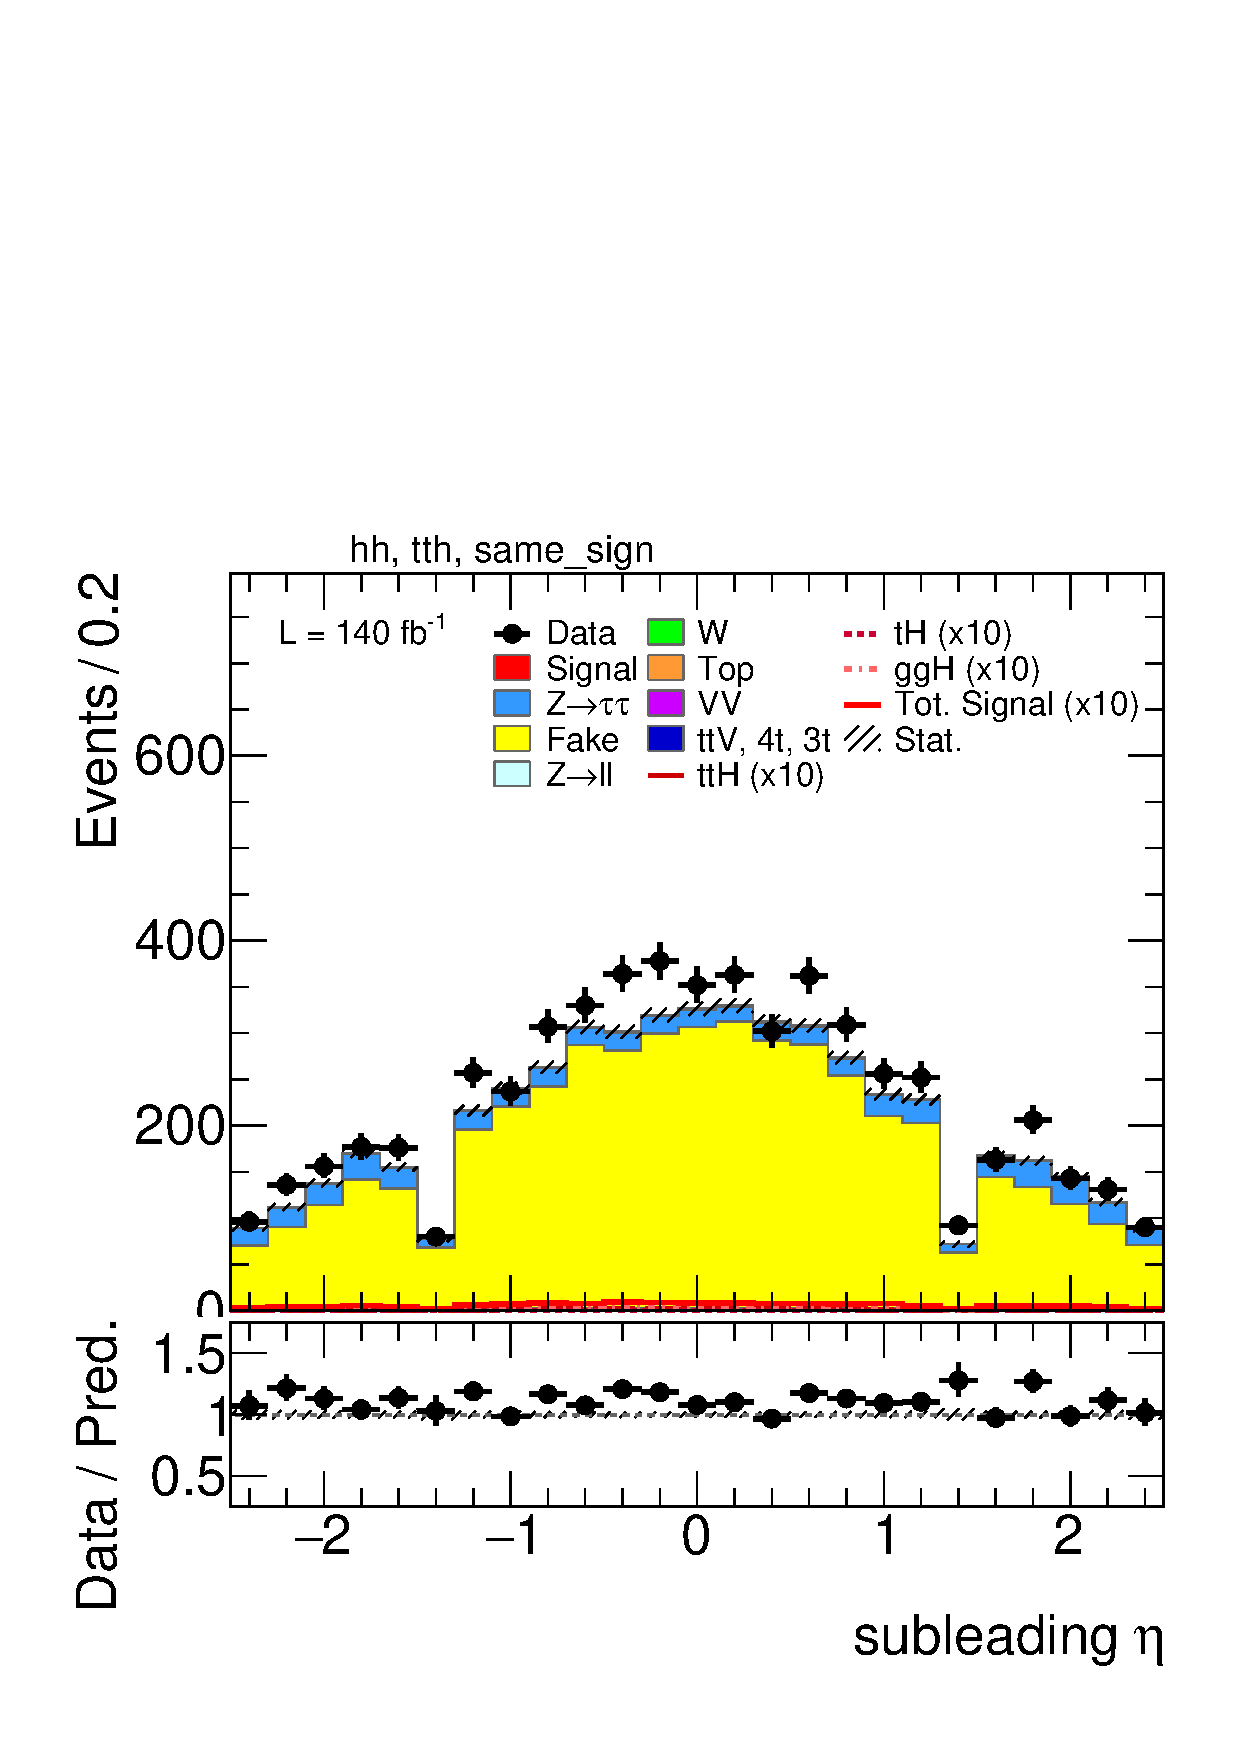
\includegraphics[width=\textwidth]{images/fakes_run2/plot_tau_1_eta_hh_tth_15_16_17_18_same_sign.pdf}
      \caption{}
    \end{subfigure}
  
    \caption{
      Closure and validation of the fake-\tauhad background estimation in Run-2 dataset, evaluated in the same-sign region at preselection level.
      The comparison is shown as a function of the \pt and $\eta$ of the leading (a), (b), and subleading (c), (d), \tauhad candidates. 
      Data are compared to the estimated fake-\tauhad background. Only statistical uncertainties are included.
    }
    \label{fig:closure_validation_run2}
  \end{figure}

  In Figure~\ref{run2_fakes_comparison}, the effect of switching from the RNN-based to the new \textsc{gntau} identification algorithm is illustrated using the data taken during 2022.
  The distributions of the jet multiplicity, as well as the \pt and $\eta$ of the leading \tauhad candidate, are shown for the preselection requiring at least one $b$-tagged jet.  
  This choice provides a more inclusive selection, ensuring sufficient statistics to clearly illustrate the effect.  
  A large reduction in the contribution from misidentified \tauhad backgrounds is observed when employing the \textsc{gntau} algorithm, highlighting its superior performance in suppressing jets misidentified as hadronic $\tau$ decays, with overall reductions of about 60-70\% compared to the previous RNN-based approach.
  
  \begin{figure}[htbp]
    \centering
    % Top row: GNTau
    \begin{subfigure}[b]{0.45\textwidth}
        \centering
        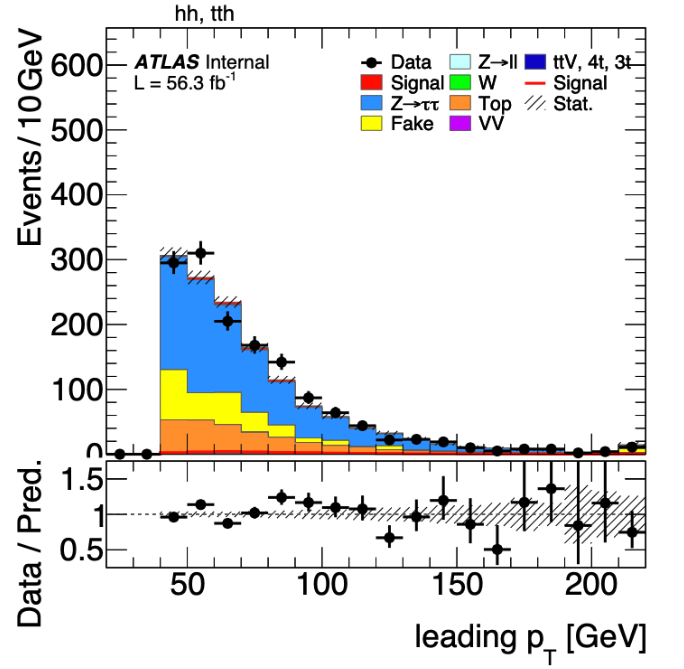
\includegraphics[width=\textwidth]{images/leading_pt_rnn.png}
        \caption{\textsc{gntau}}
    \end{subfigure}
    \begin{subfigure}[b]{0.45\textwidth}
        \centering
        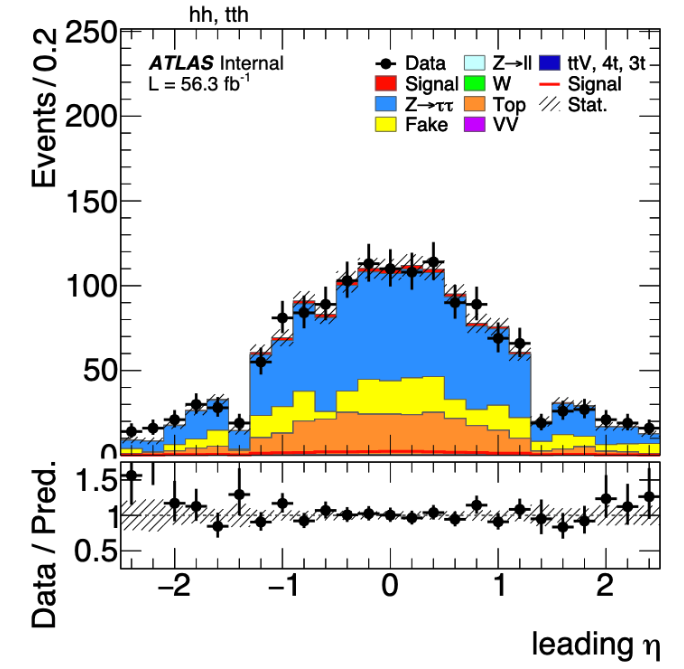
\includegraphics[width=\textwidth]{images/leading_eta_rnn.png}
        \caption{\textsc{gntau}}
    \end{subfigure}

    % Bottom row: RNN
    \begin{subfigure}[b]{0.45\textwidth}
        \centering
        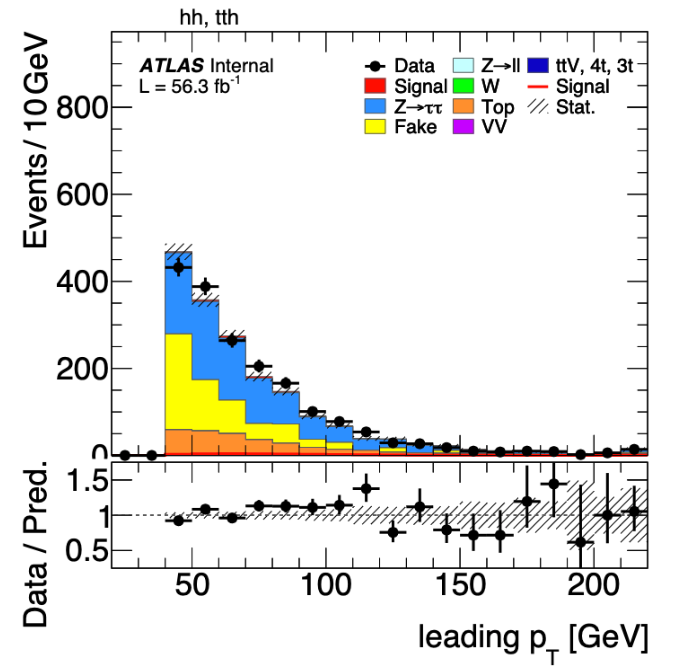
\includegraphics[width=\textwidth]{images/leading_pt_gntau.png}
        \caption{RNN-ID}
    \end{subfigure}
    \begin{subfigure}[b]{0.45\textwidth}
        \centering
        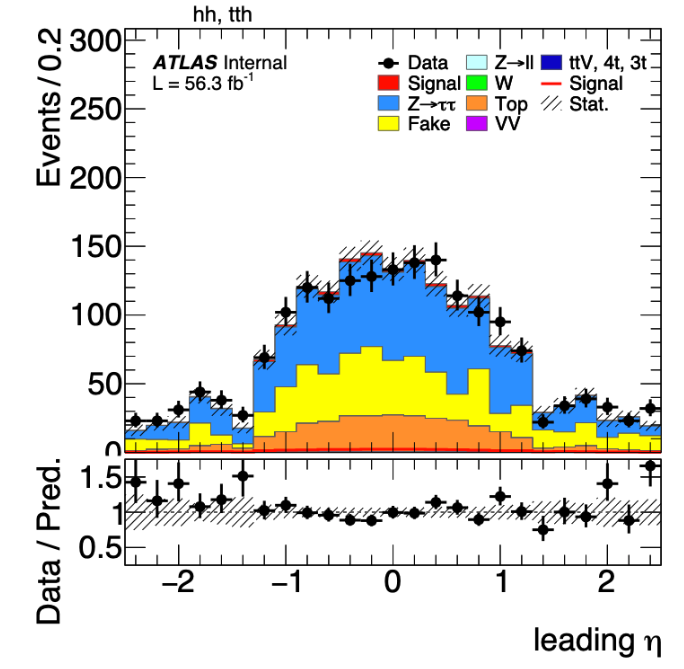
\includegraphics[width=\textwidth]{images/leading_eta_gntau.png}
        \caption{RNN-ID}
    \end{subfigure}

    \caption{Distributions of the leading \tauhad candidate transverse momentum and pseudorapidity at the \ttH preselection with at least one $b$-tagged jet. 
    The upper row shows the results obtained with the new \textsc{GNTau} identification algorithm (a) and (b), while the lower row shows the corresponding distributions with the previously used RNN-based approach (c) and (d). These distributions are evaluated on data and simulations from 2022 data-taking periond. Scaling factors on \ztautau and \ttbar are applied. Only statistical uncertainties are included.}
    \label{run2_fakes_comparison}
\end{figure}

\subsection{Systematic variations}

The variations contributing to the systematic uncertainties in the fake-\tauhad background estimation have been reevaluated (such as the composition and parametrization uncertainty sources,  discussed in Section~\ref{sec:event_selection_background}).
To account for differences in background composition, two alternative CRs were defined. 

The first corresponds to the selection of same-sign events, which are naturally enriched in jets misidentified as \tauhad, predominantly originating from QCD multi-jet production, as mentioned before.
The second alternative is the high-$\Delta\eta(\tau_0,\tau_1)$ region, $1.5 < \Delta\eta < 2.0$, which is more sensitive to dijet-like topologies. In this case, the presence of forward jets with low track multiplicity enhances the probability of jets being misidentified as \tauhad candidates, thus providing an additional validation of the robustness of the method. The closure obtained when estimating this background contribution with these alternative CRs is shown in Figures~\ref{fig:closure_validation_same_sign_run3} and~\ref{fig:closure_validation_same_sign_run2} for the same-sign composition uncertainties, evaluated in the same-sign \tauhadhad signal phase-space, and in Figures~\ref{fig:closure_validation_highdeta_run3} and~\ref{fig:closure_validation_highdeta_run2} it is shown the analogous representation in the high-$\Delta \eta (\tau_0,\tau_1)$ case.

From these results, it can be concluded that the estimation of the fake-\tauhad background is fairly accurate when using either of the alternative control regions. Both the high-$\Delta\eta(\tau_0,\tau_1)$ and the same-sign regions provide consistent and reliable predictions for the overall Fake contribution compared to the nominal approach
%Run_3 same_sign closure
\begin{figure}[htbp]
  \centering
  \begin{subfigure}[b]{0.45\textwidth}
    \centering
    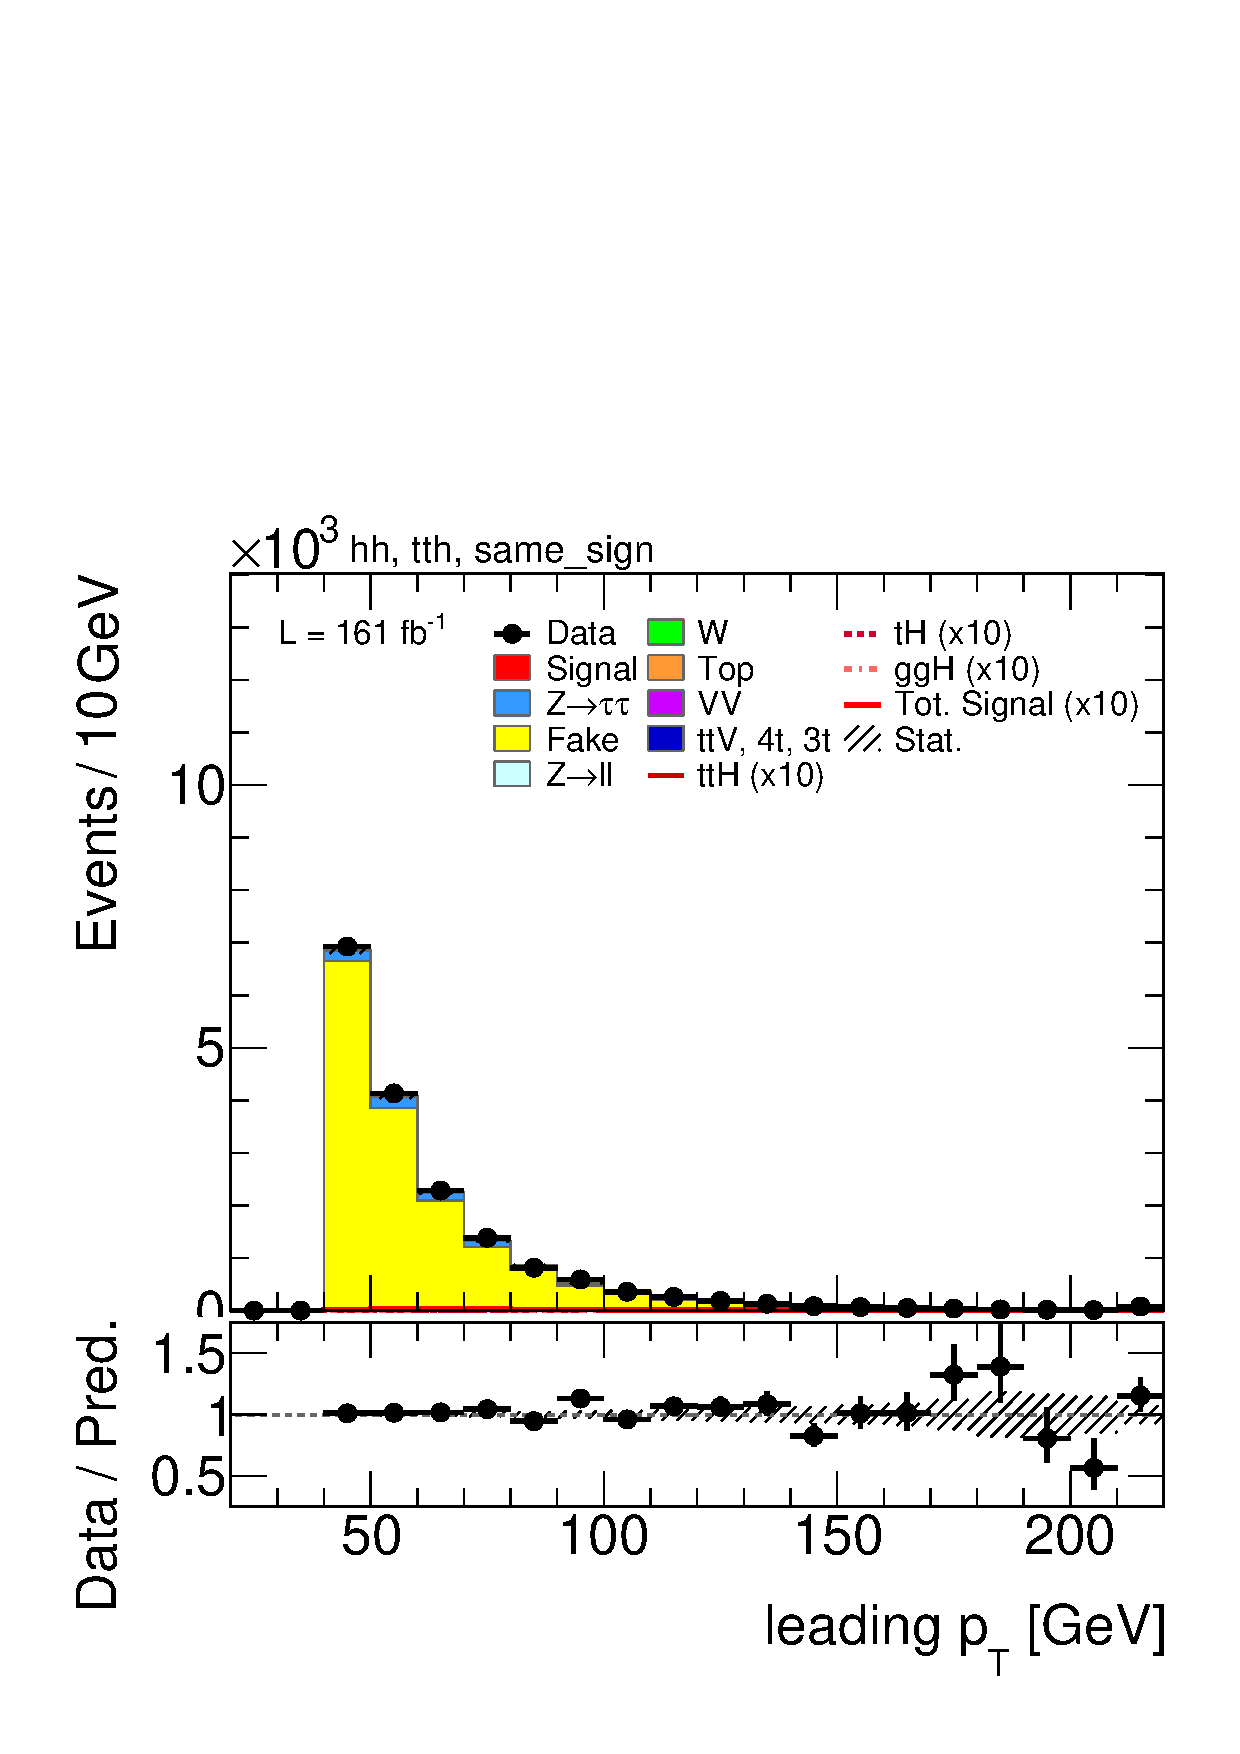
\includegraphics[width=\textwidth]{images/same_sign_same_sign_run3/plot_tau_0_pt_hh_tth_22_23_24_same_sign.pdf}
    \caption{}
  \end{subfigure}
  \hfill
  \begin{subfigure}[b]{0.45\textwidth}
    \centering
    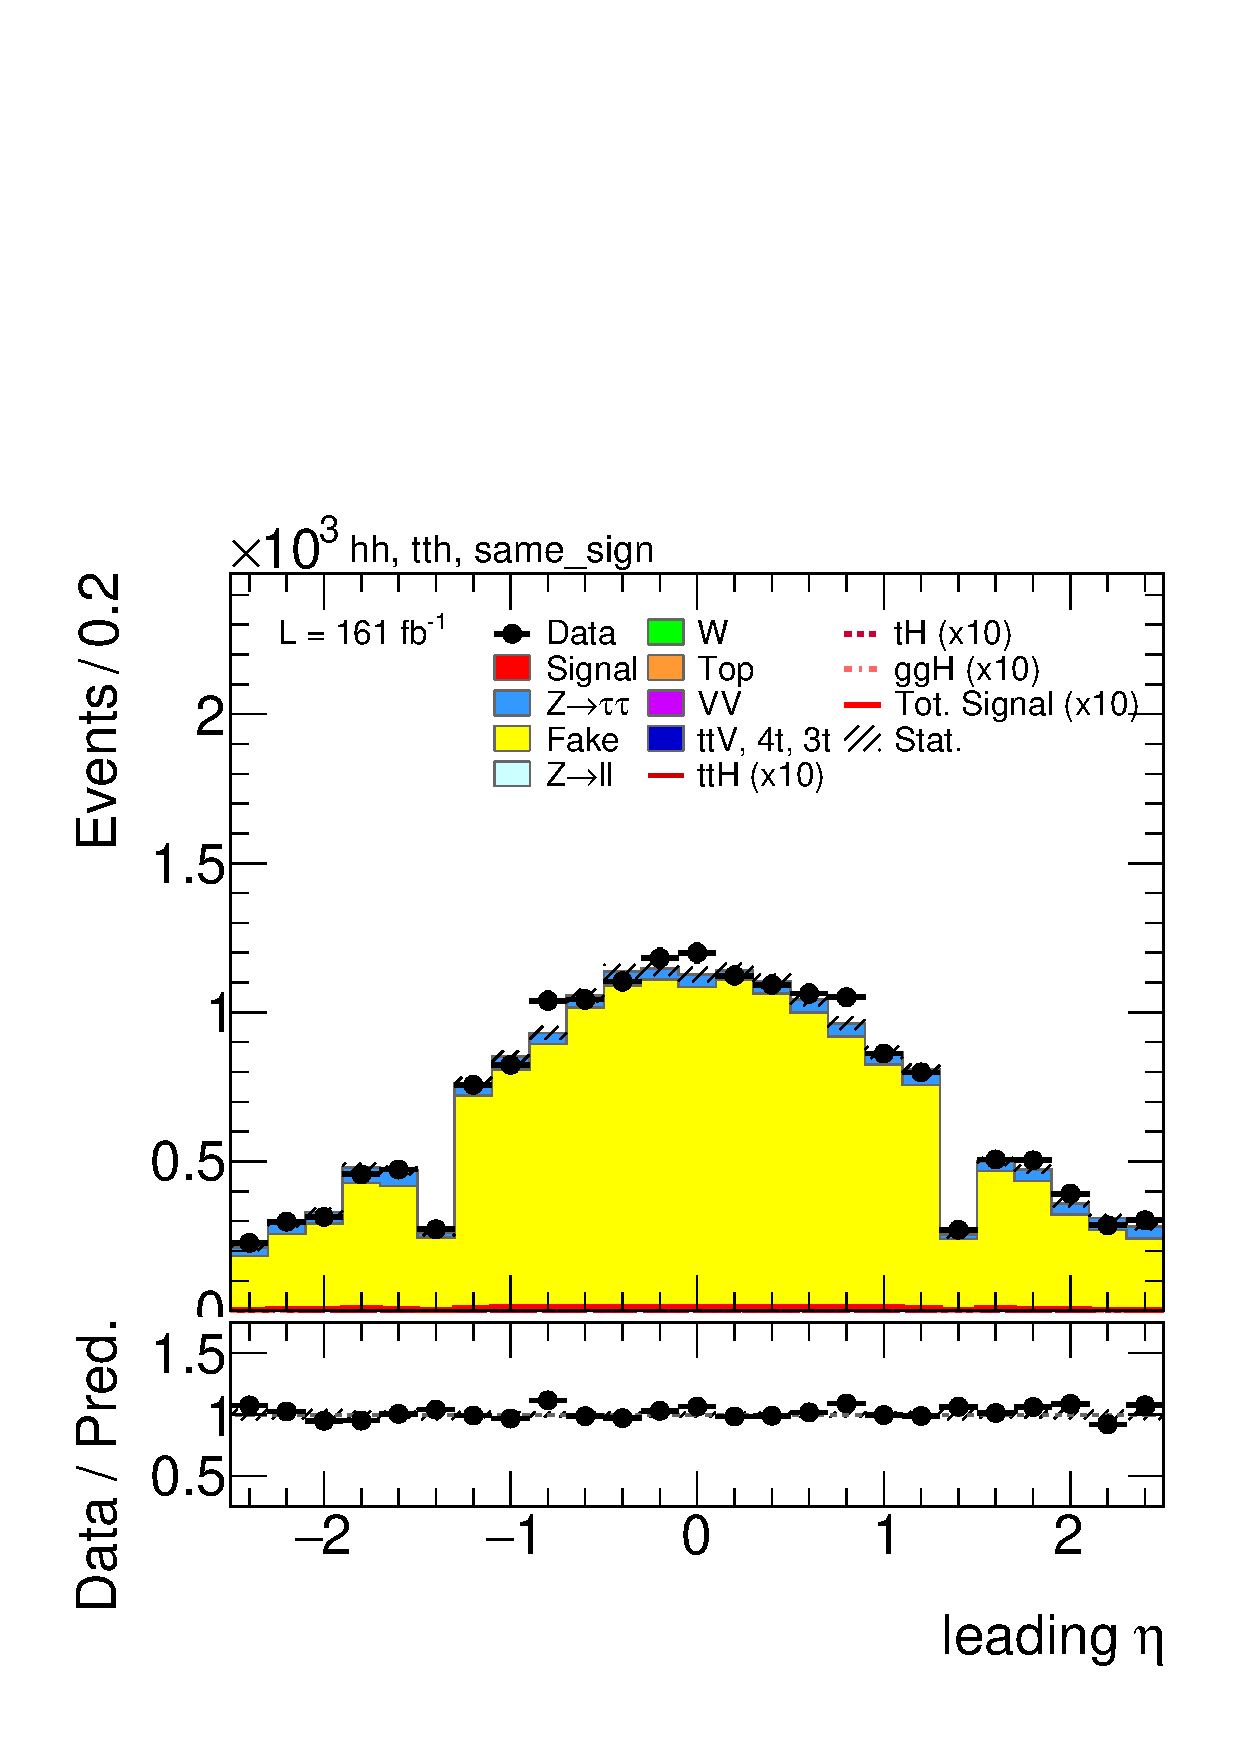
\includegraphics[width=\textwidth]{images/same_sign_same_sign_run3/plot_tau_0_eta_hh_tth_22_23_24_same_sign.pdf}
    \caption{}
  \end{subfigure}


  \begin{subfigure}[b]{0.45\textwidth}
    \centering
    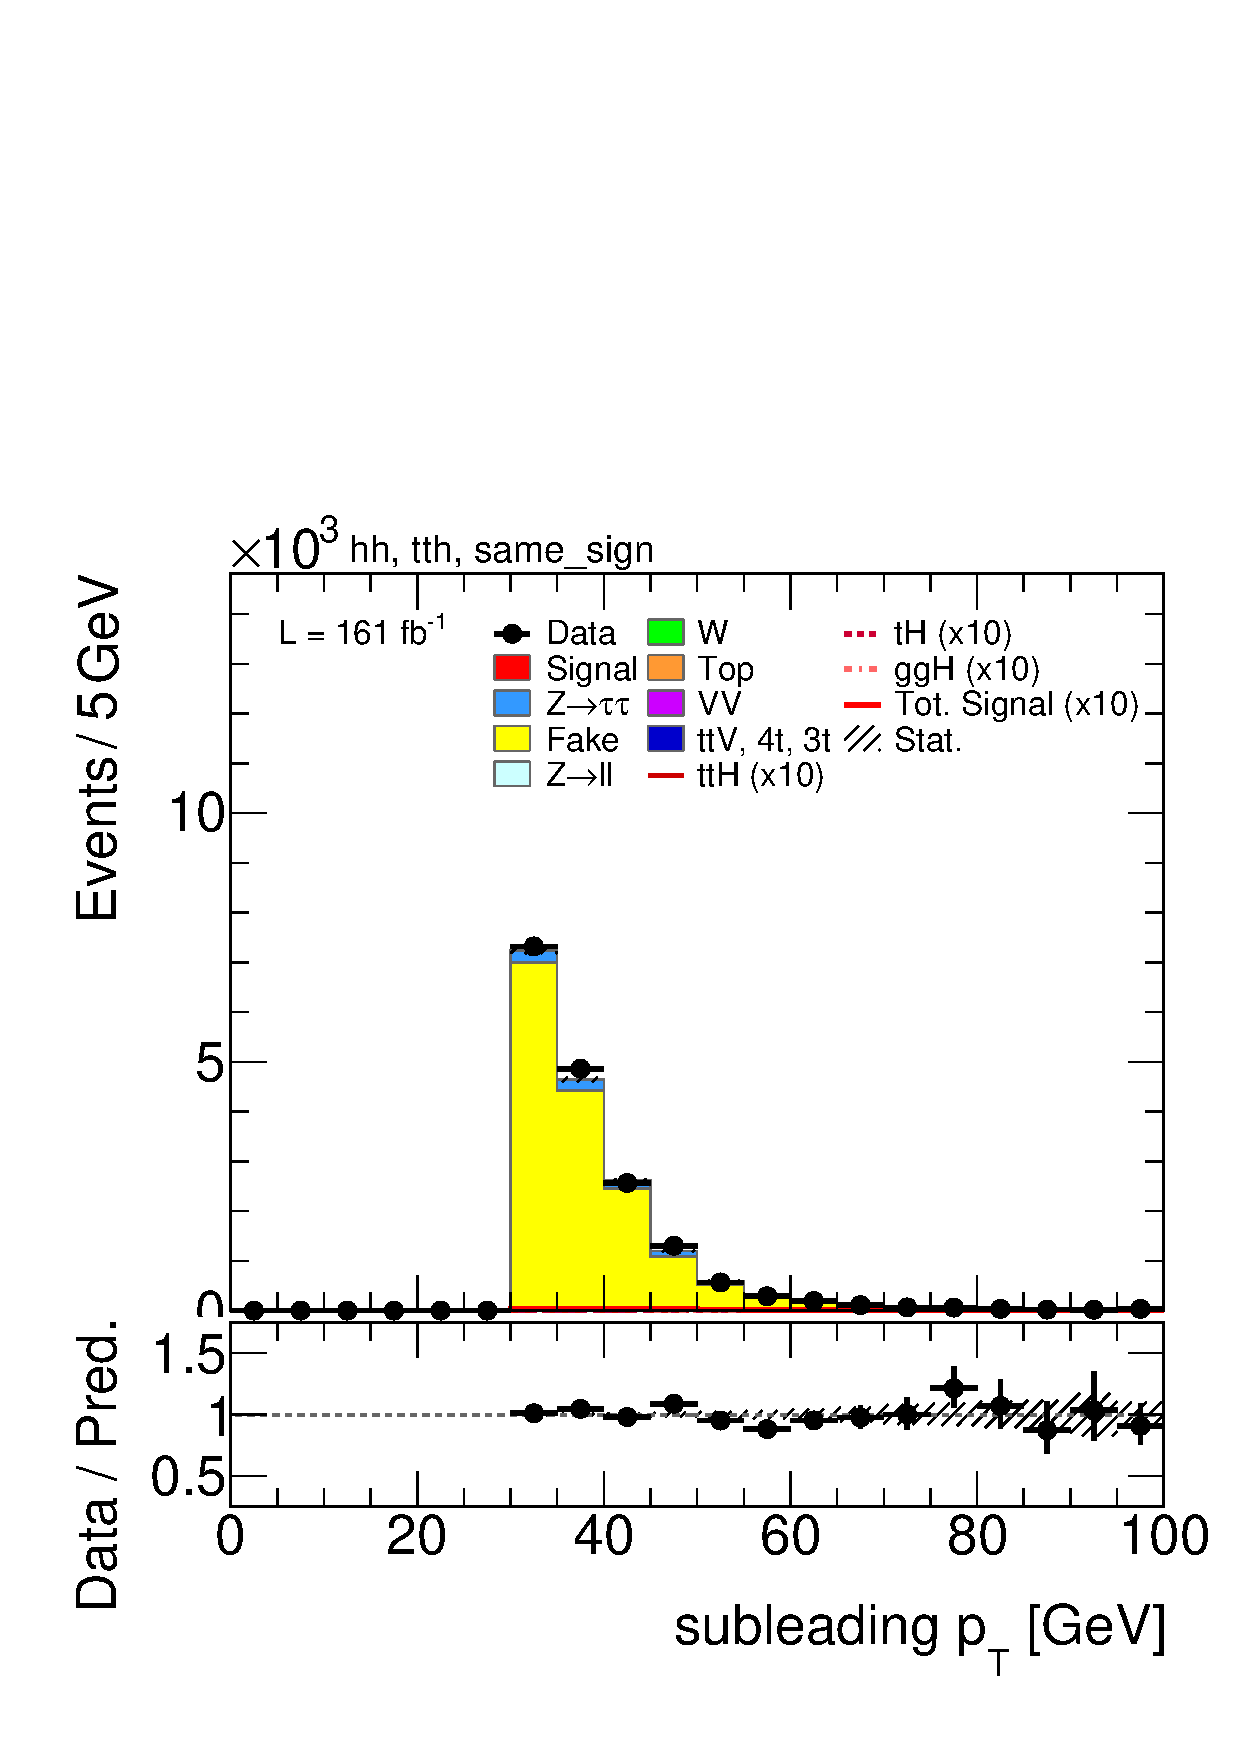
\includegraphics[width=\textwidth]{images/same_sign_same_sign_run3/plot_tau_1_pt_hh_tth_22_23_24_same_sign.pdf}
    \caption{}
  \end{subfigure}
  \hfill
  \begin{subfigure}[b]{0.45\textwidth}
    \centering
    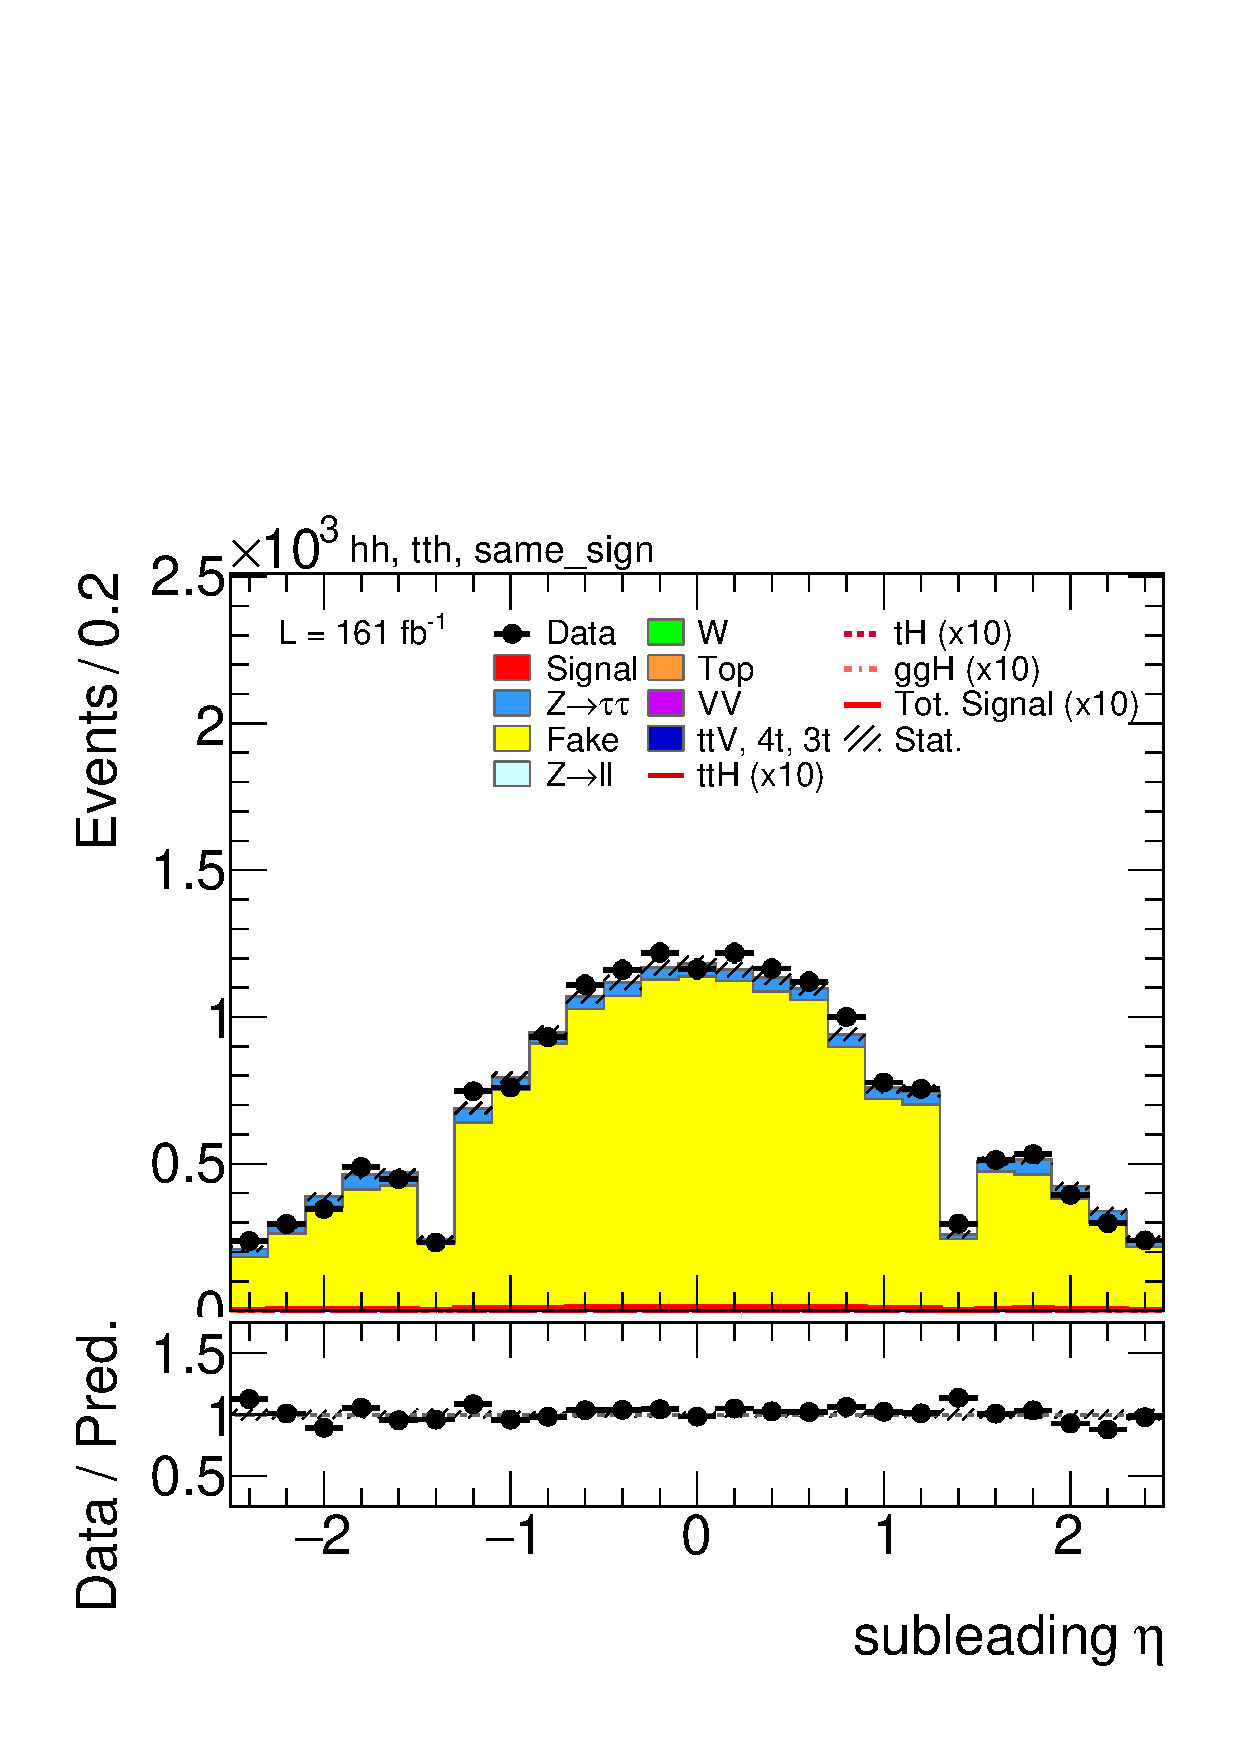
\includegraphics[width=\textwidth]{images/same_sign_same_sign_run3/plot_tau_1_eta_hh_tth_22_23_24_same_sign.pdf}
    \caption{}
  \end{subfigure}
  \caption{
    Closure and validation of the fake-\tauhad background estimated in Run-3 dataset with the alternative same-sign \tauhadhad CR, evaluated in the same-sign region at preselection level.
    The comparison is shown as a function of the \pt and $\eta$ of the leading (a), (b), and subleading (c), (d), \tauhad candidates. 
    Data are compared to the estimated fake-\tauhad background. Scaling factors on \ztautau and \ttbar are applied. Only statistical uncertainties are included.
  }
  \label{fig:closure_validation_same_sign_run3}
\end{figure}
  
  
  %Run_2 same_sign closure
  \begin{figure}[htbp]
    \centering
    \begin{subfigure}[b]{0.45\textwidth}
      \centering
      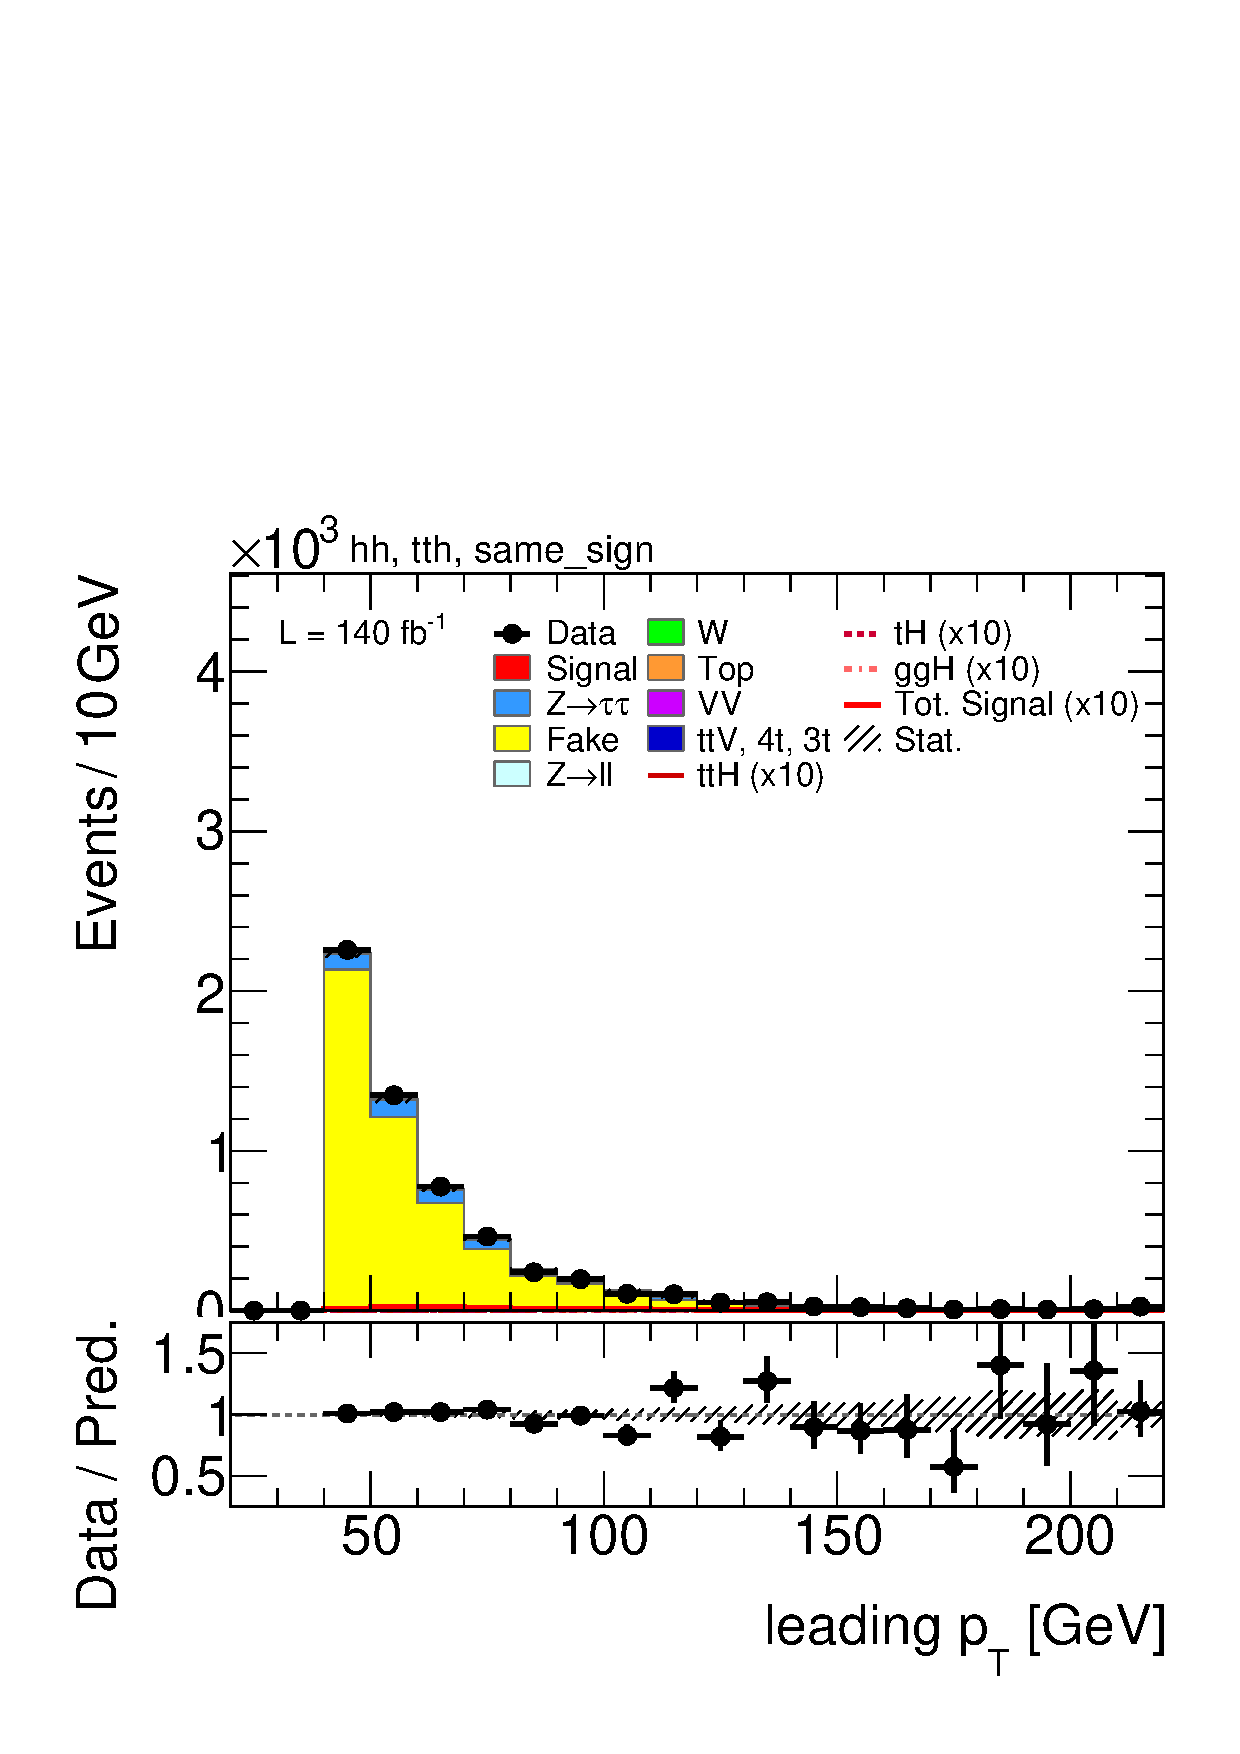
\includegraphics[width=\textwidth]{images/same_sign_same_sign_run2/plot_tau_0_pt_hh_tth_15_16_17_18_same_sign.pdf}
      \caption{}
    \end{subfigure}
    \hfill
    \begin{subfigure}[b]{0.45\textwidth}
      \centering
      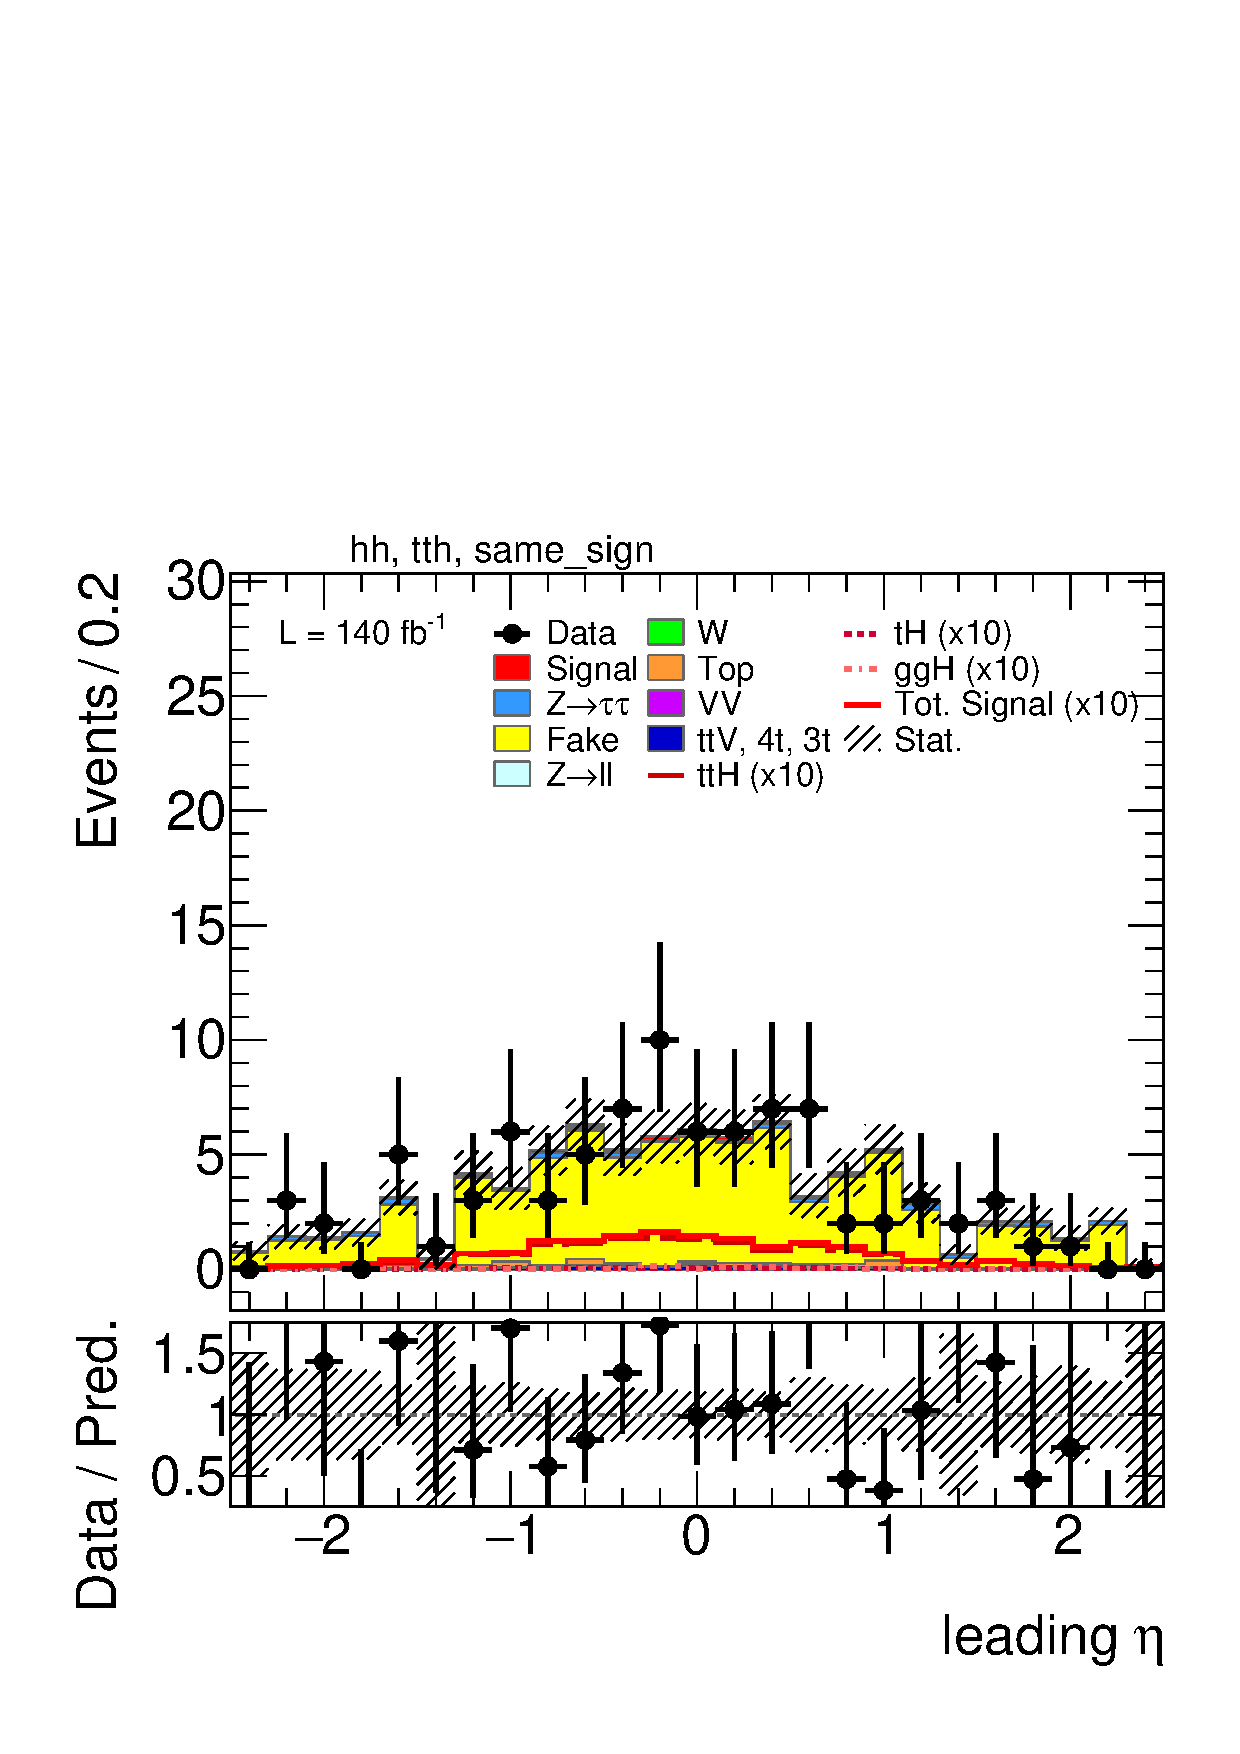
\includegraphics[width=\textwidth]{images/same_sign_same_sign_run2/plot_tau_0_eta_hh_tth_15_16_17_18_same_sign.pdf}
      \caption{}
    \end{subfigure}

    \begin{subfigure}[b]{0.45\textwidth}
      \centering
      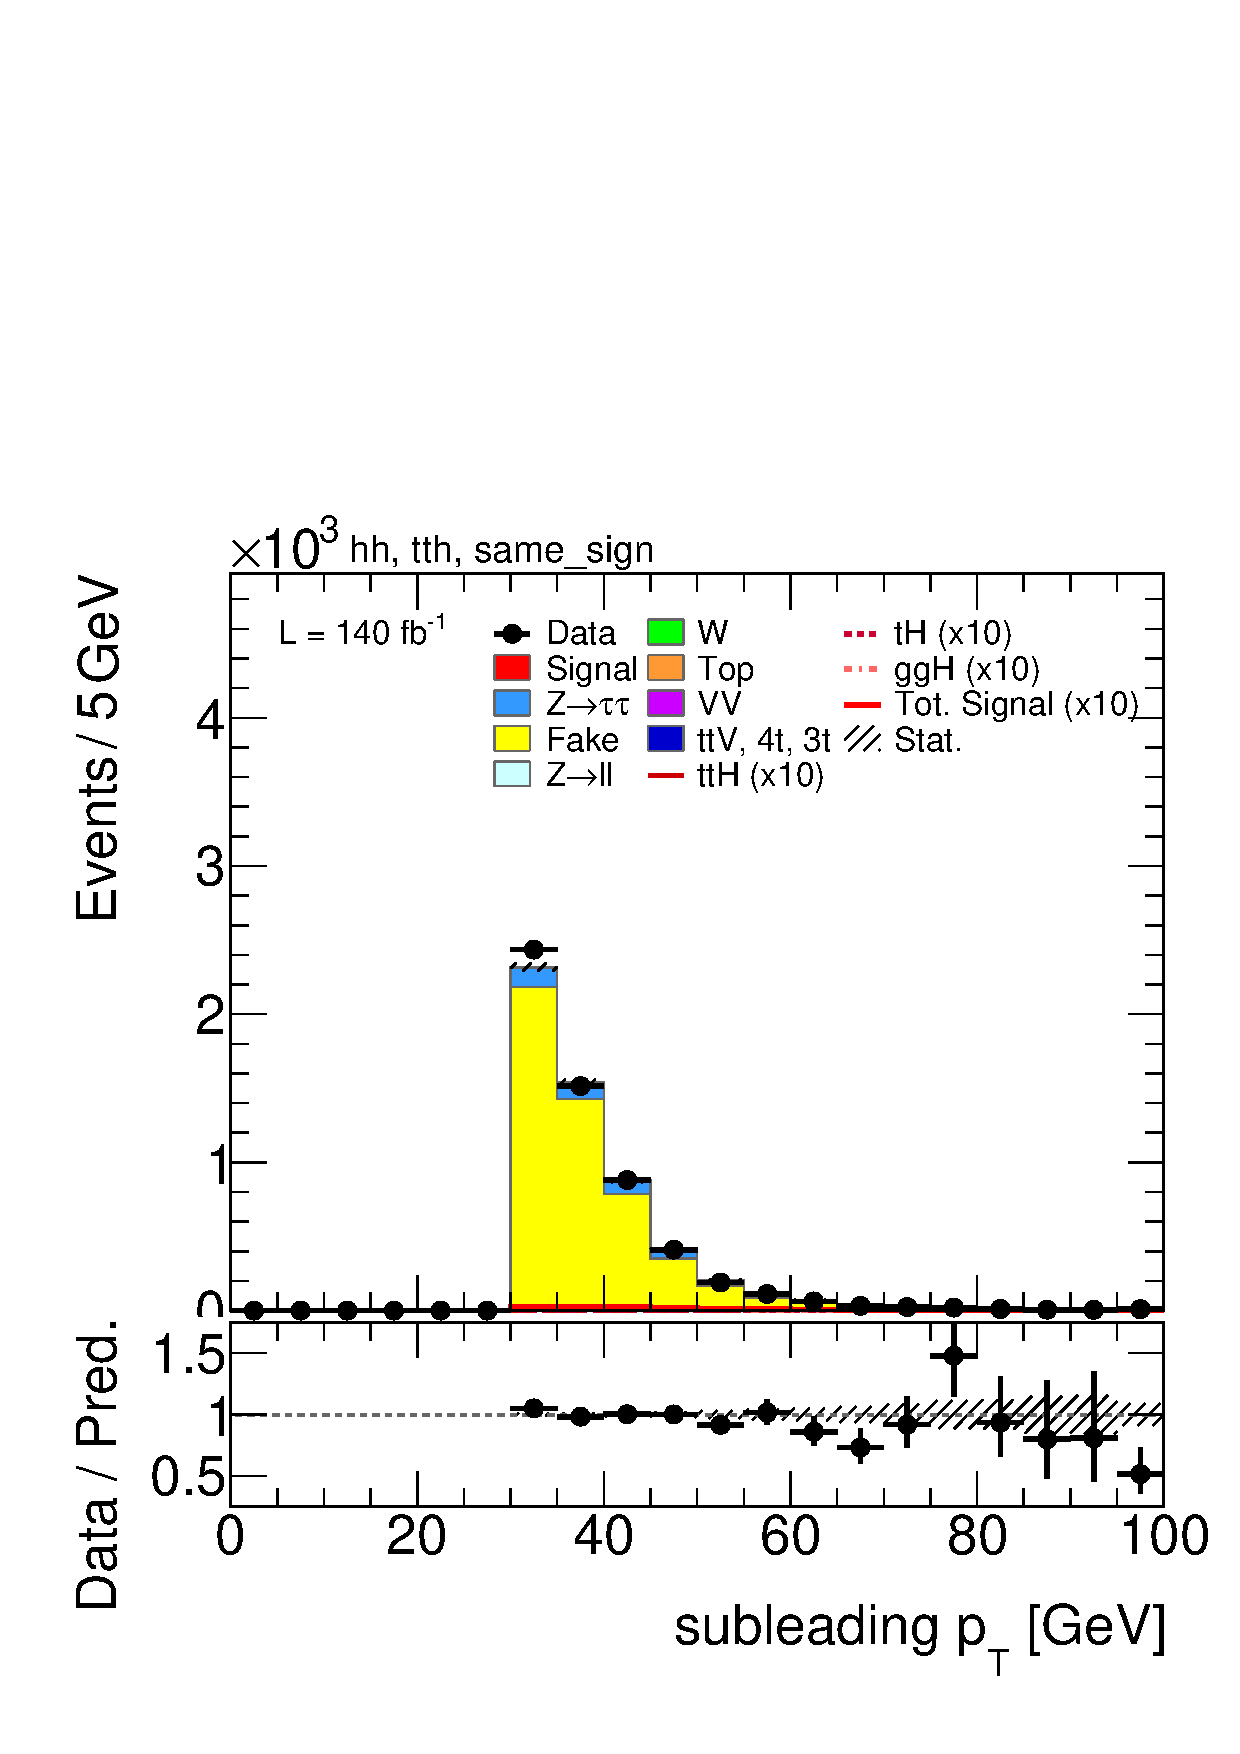
\includegraphics[width=\textwidth]{images/same_sign_same_sign_run2/plot_tau_1_pt_hh_tth_15_16_17_18_same_sign.pdf}
      \caption{}
    \end{subfigure}
    \hfill
    \begin{subfigure}[b]{0.45\textwidth}
      \centering
      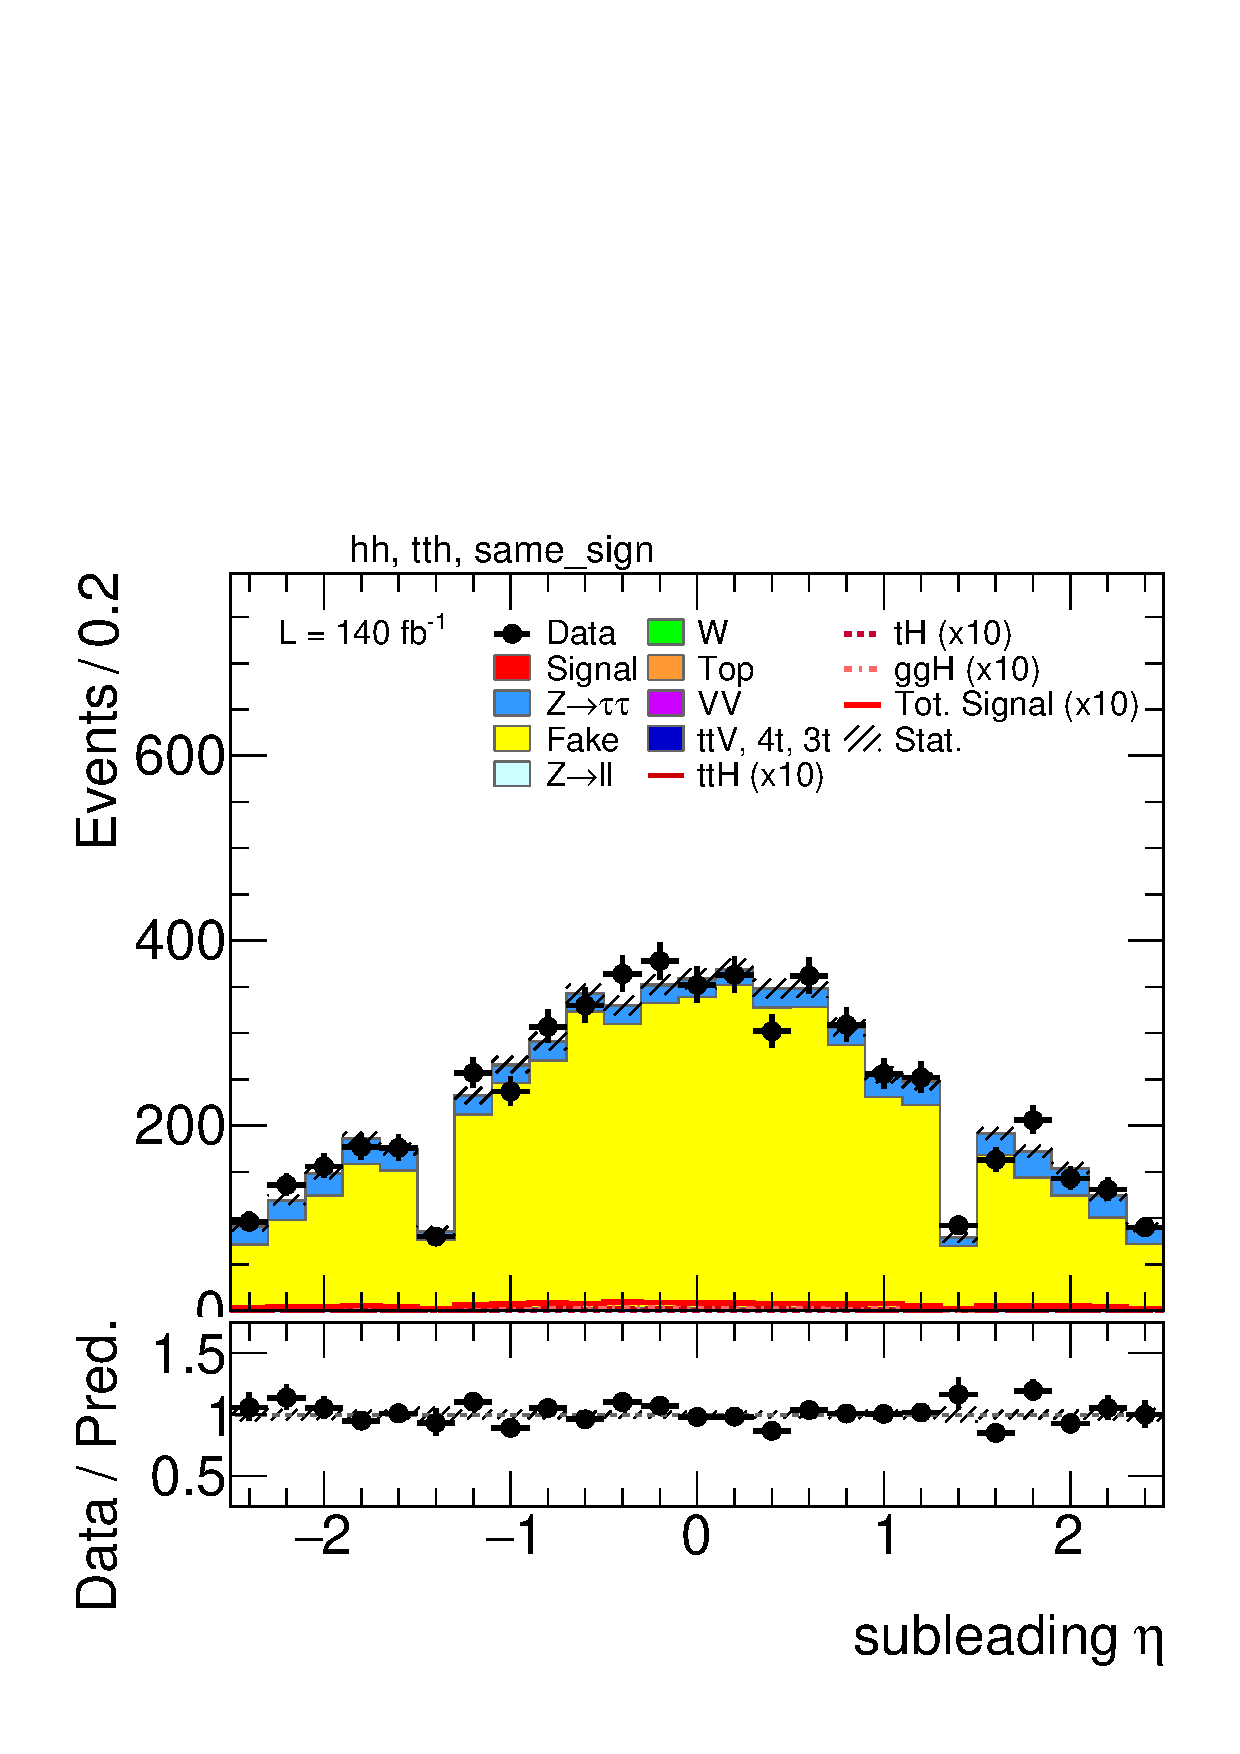
\includegraphics[width=\textwidth]{images/same_sign_same_sign_run2/plot_tau_1_eta_hh_tth_15_16_17_18_same_sign.pdf}
      \caption{}
    \end{subfigure}

    \caption{
    Closure and validation of the fake-\tauhad background estimated in Run-2 dataset with the alternative same-sign \tauhadhad CR, evaluated in the same-sign region at preselection level.
    The comparison is shown as a function of the \pt and $\eta$ of the leading (a), (b), and subleading (c), (d), \tauhad candidates. Only statistical uncertainties are included.
    Data are compared to the estimated fake-\tauhad background.
  }
  \label{fig:closure_validation_same_sign_run2}
\end{figure}

    %Run_3 high_deta closure
    \begin{figure}[htbp]
      \centering
      \begin{subfigure}[b]{0.45\textwidth}
        \centering
        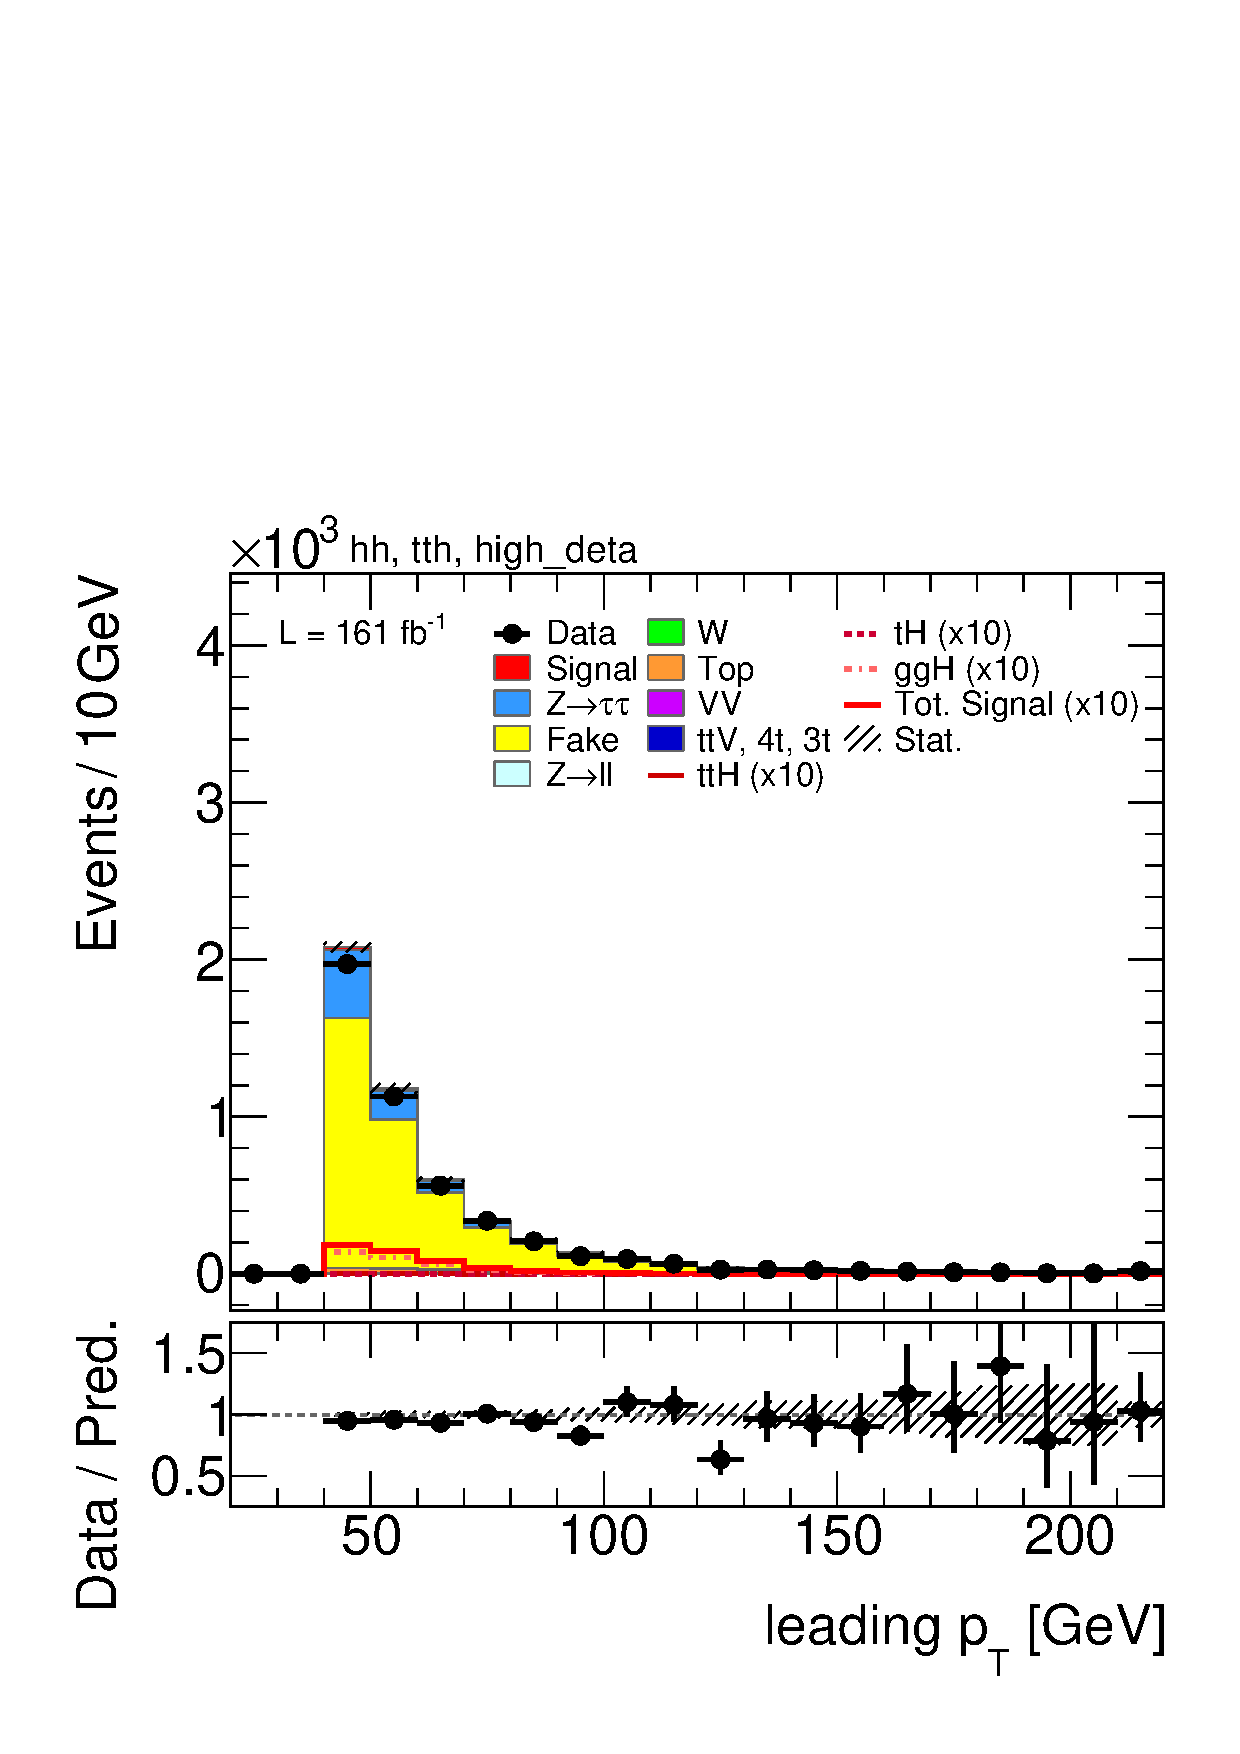
\includegraphics[width=\textwidth]{images/using_highdeta_ffs_run3_inclusive_withscaling/plot_tau_0_pt_hh_tth_22_23_24_high_deta.pdf}
        \caption{}
      \end{subfigure}
      \hfill
      \begin{subfigure}[b]{0.45\textwidth}
        \centering
        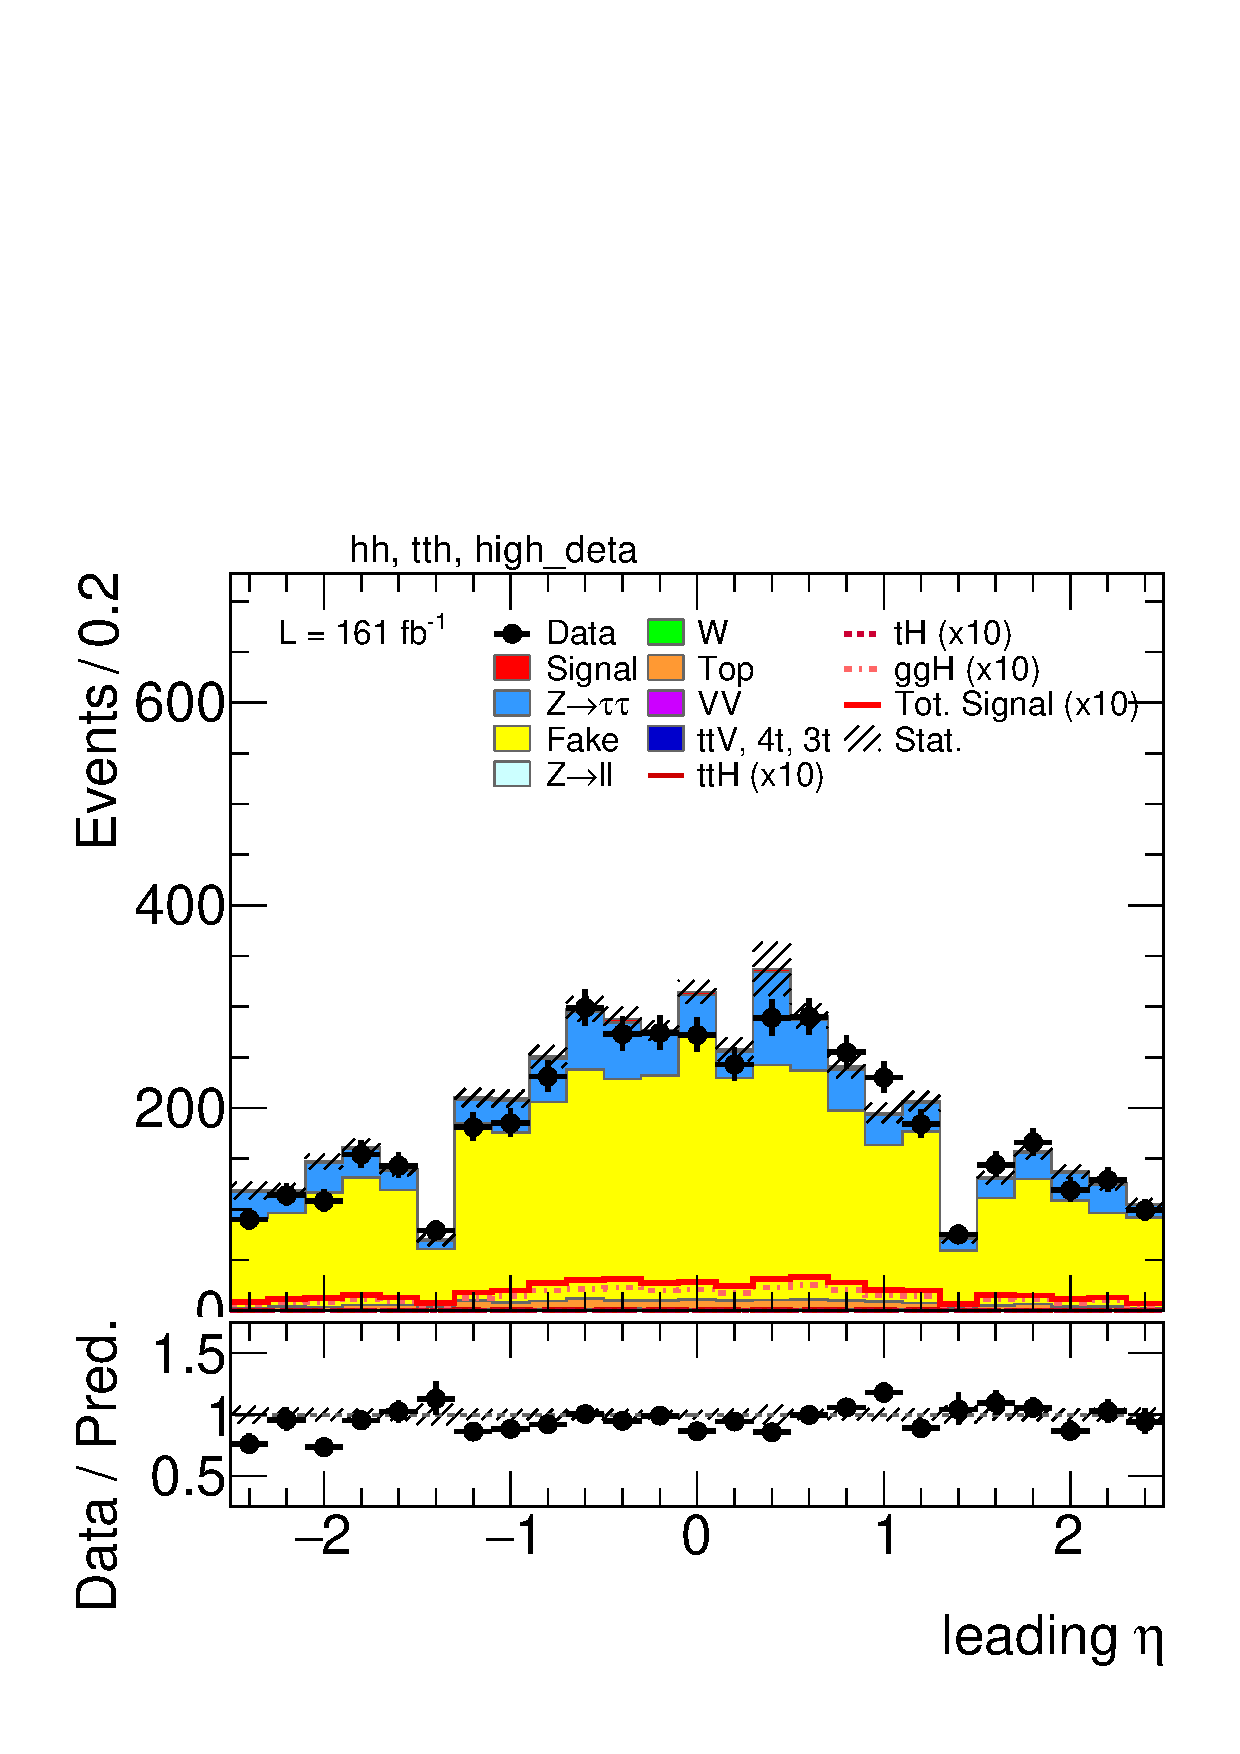
\includegraphics[width=\textwidth]{images/using_highdeta_ffs_run3_inclusive_withscaling/plot_tau_0_eta_hh_tth_22_23_24_high_deta.pdf}
        \caption{}
      \end{subfigure}
  
      \begin{subfigure}[b]{0.45\textwidth}
        \centering
        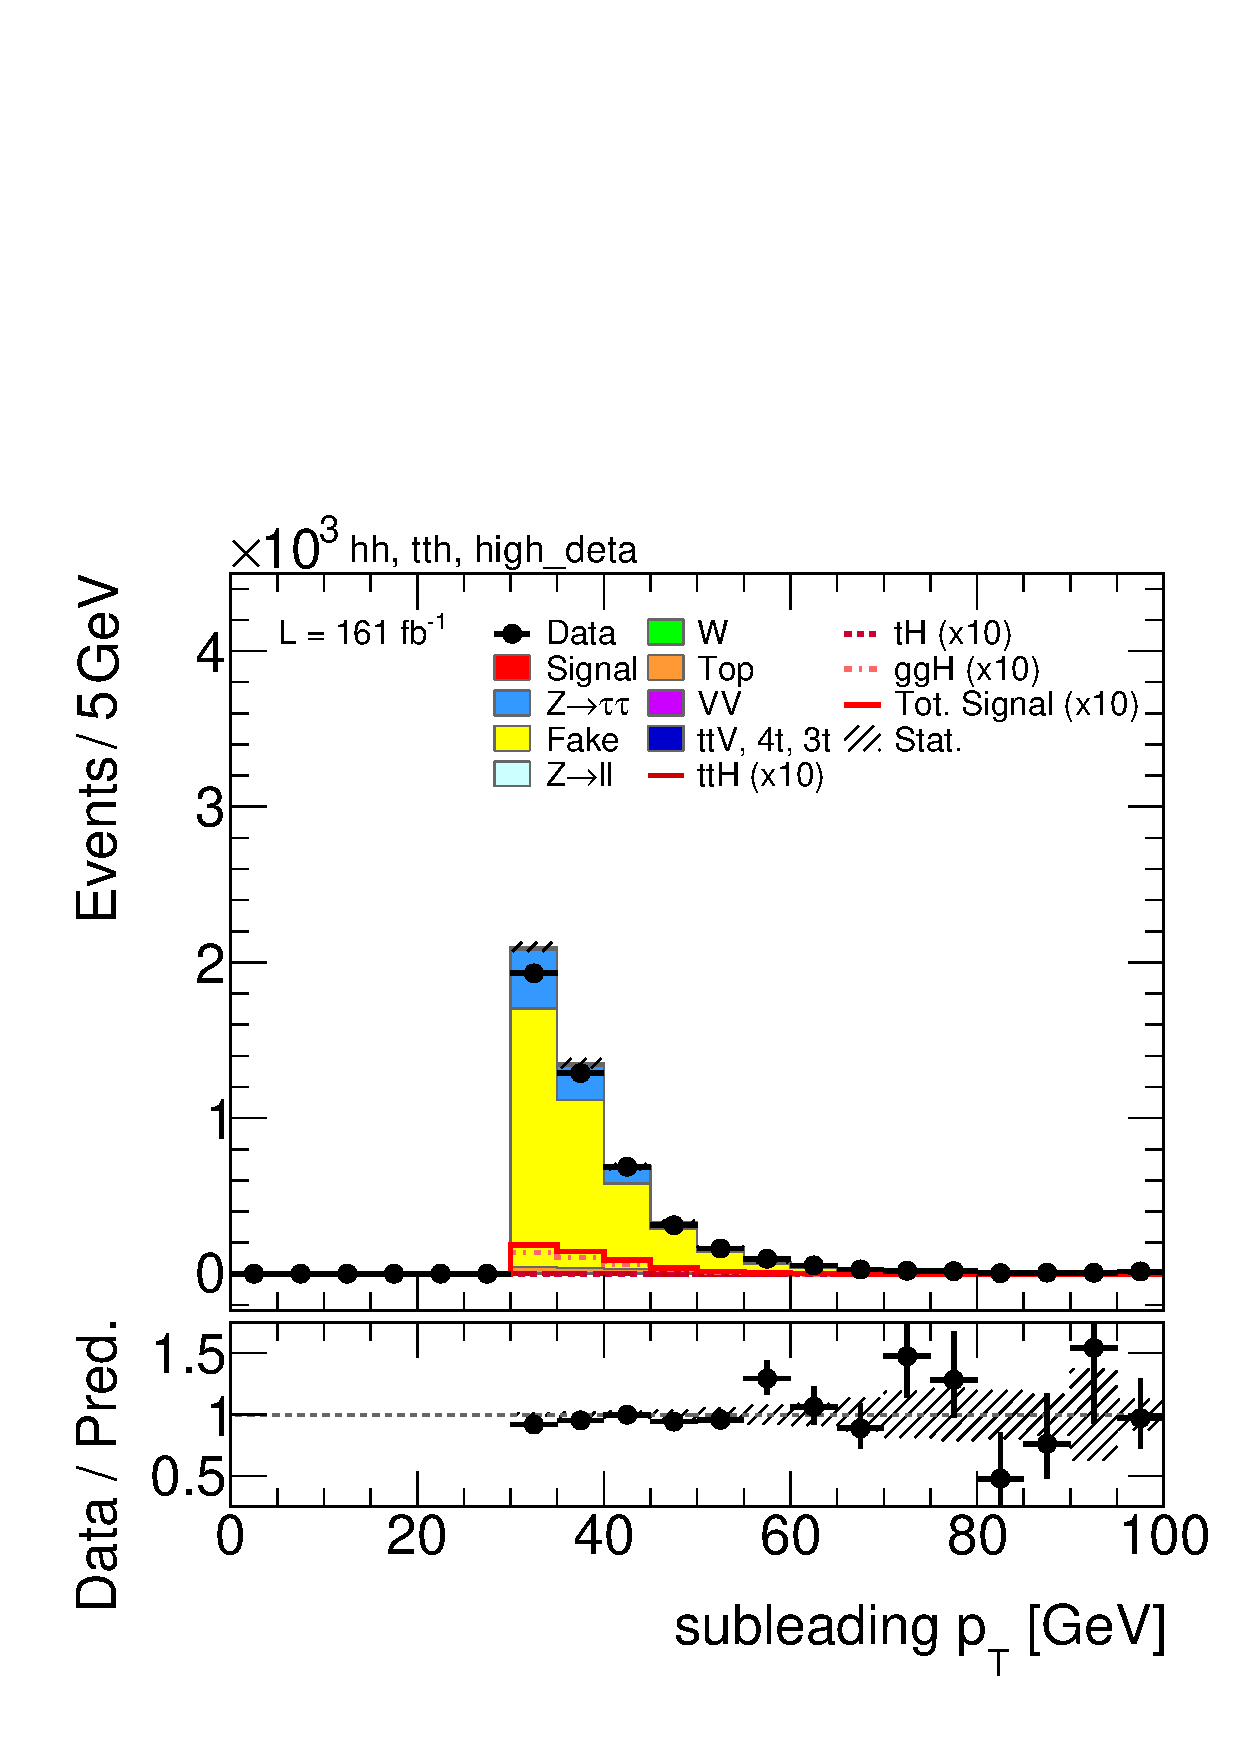
\includegraphics[width=\textwidth]{images/using_highdeta_ffs_run3_inclusive_withscaling/plot_tau_1_pt_hh_tth_22_23_24_high_deta.pdf}
        \caption{}
      \end{subfigure}
      \hfill
      \begin{subfigure}[b]{0.45\textwidth}
        \centering
        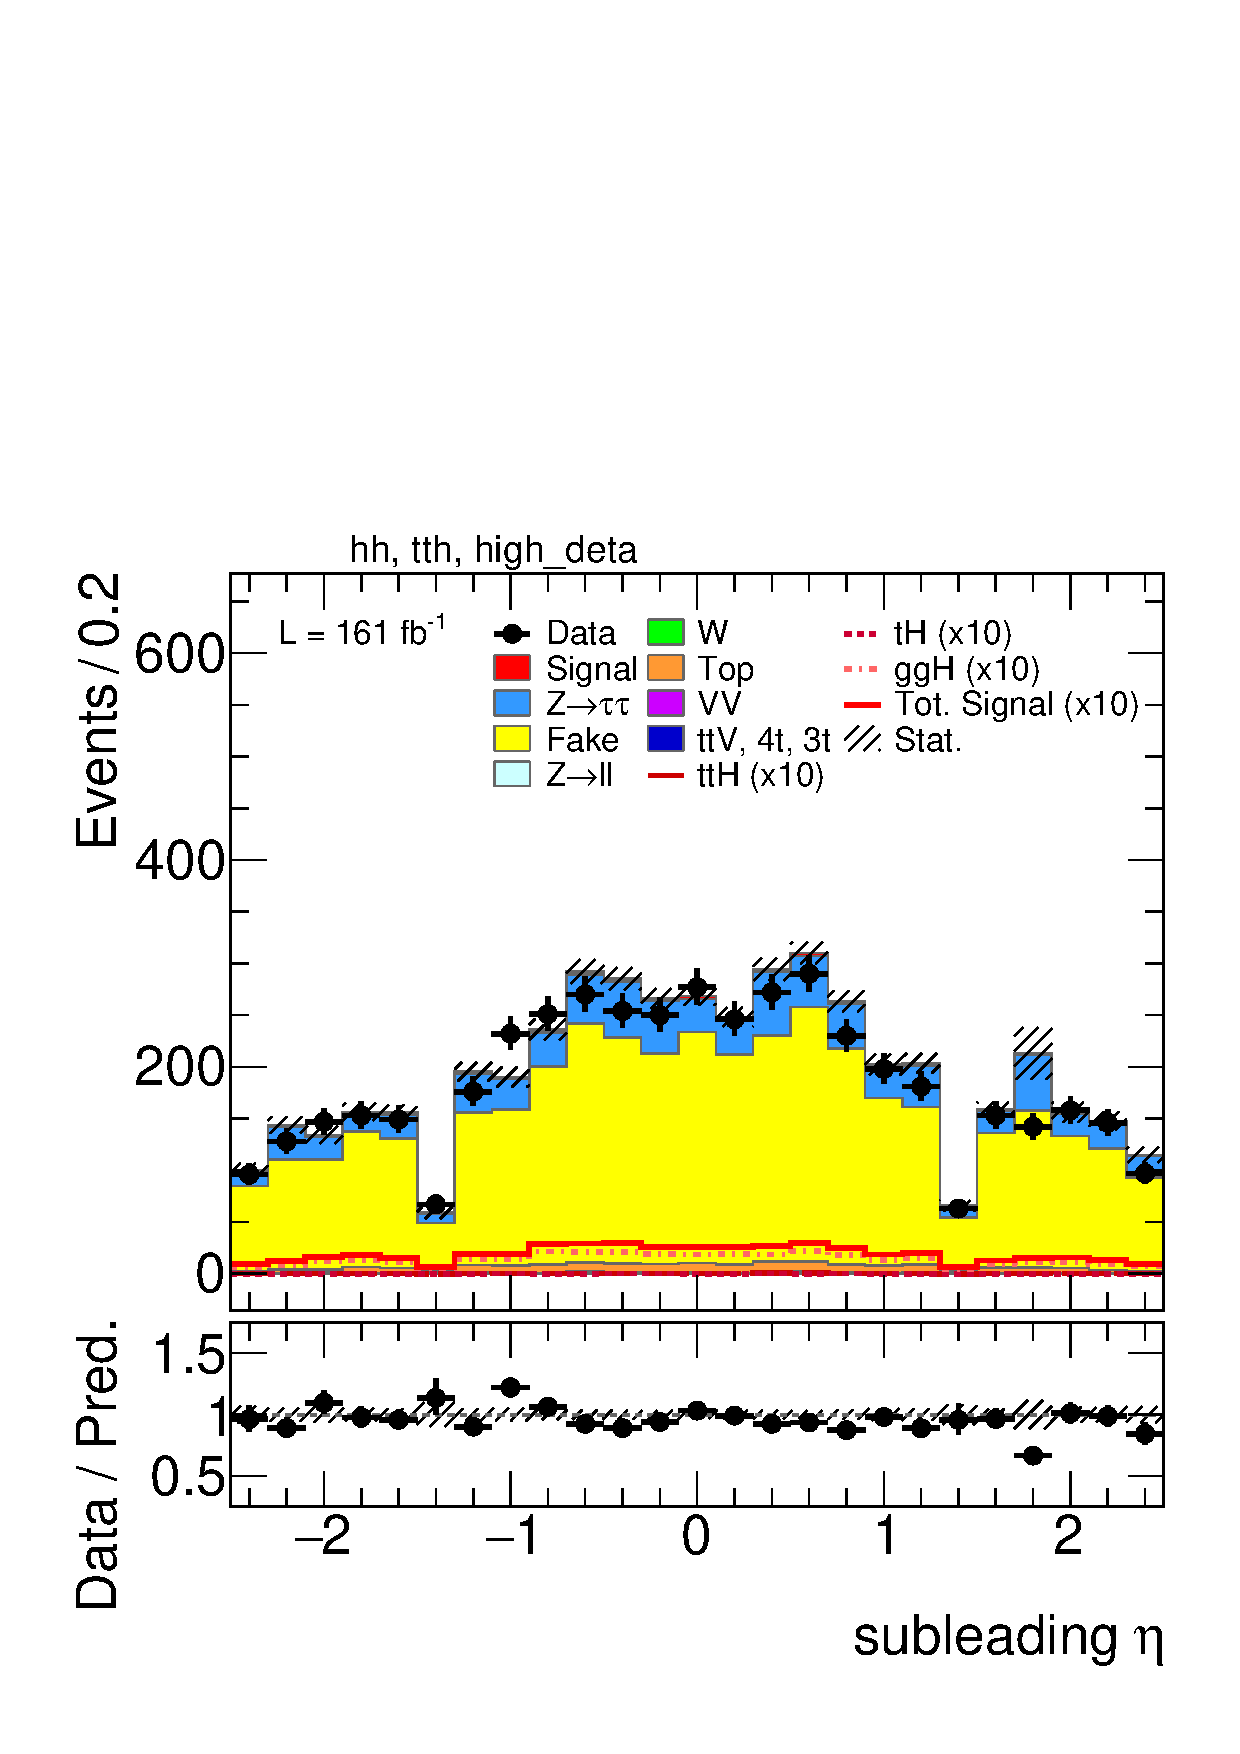
\includegraphics[width=\textwidth]{images/using_highdeta_ffs_run3_inclusive_withscaling/plot_tau_1_eta_hh_tth_22_23_24_high_deta.pdf}
        \caption{}
      \end{subfigure}
      \caption{
    Closure and validation of the fake-\tauhad background estimated in Run-3 dataset with the alternative high-$\Delta \eta (\tau_0, \tau_1)$ \tauhadhad CR, evaluated in the high-$\Delta \eta (\tau_0, \tau_1)$ region at preselection level.
    The comparison is shown as a function of the \pt and $\eta$ of the leading (a), (b), and subleading (c), (d), \tauhad candidates. 
    Data are compared to the estimated fake-\tauhad background. Scaling factors on \ztautau and \ttbar are applied. Only statistical uncertainties are included.
  }
  \label{fig:closure_validation_highdeta_run3}
\end{figure}
      

      %Run_2 high_deta closure
      \begin{figure}[htbp]
        \centering
        \begin{subfigure}[b]{0.45\textwidth}
          \centering
          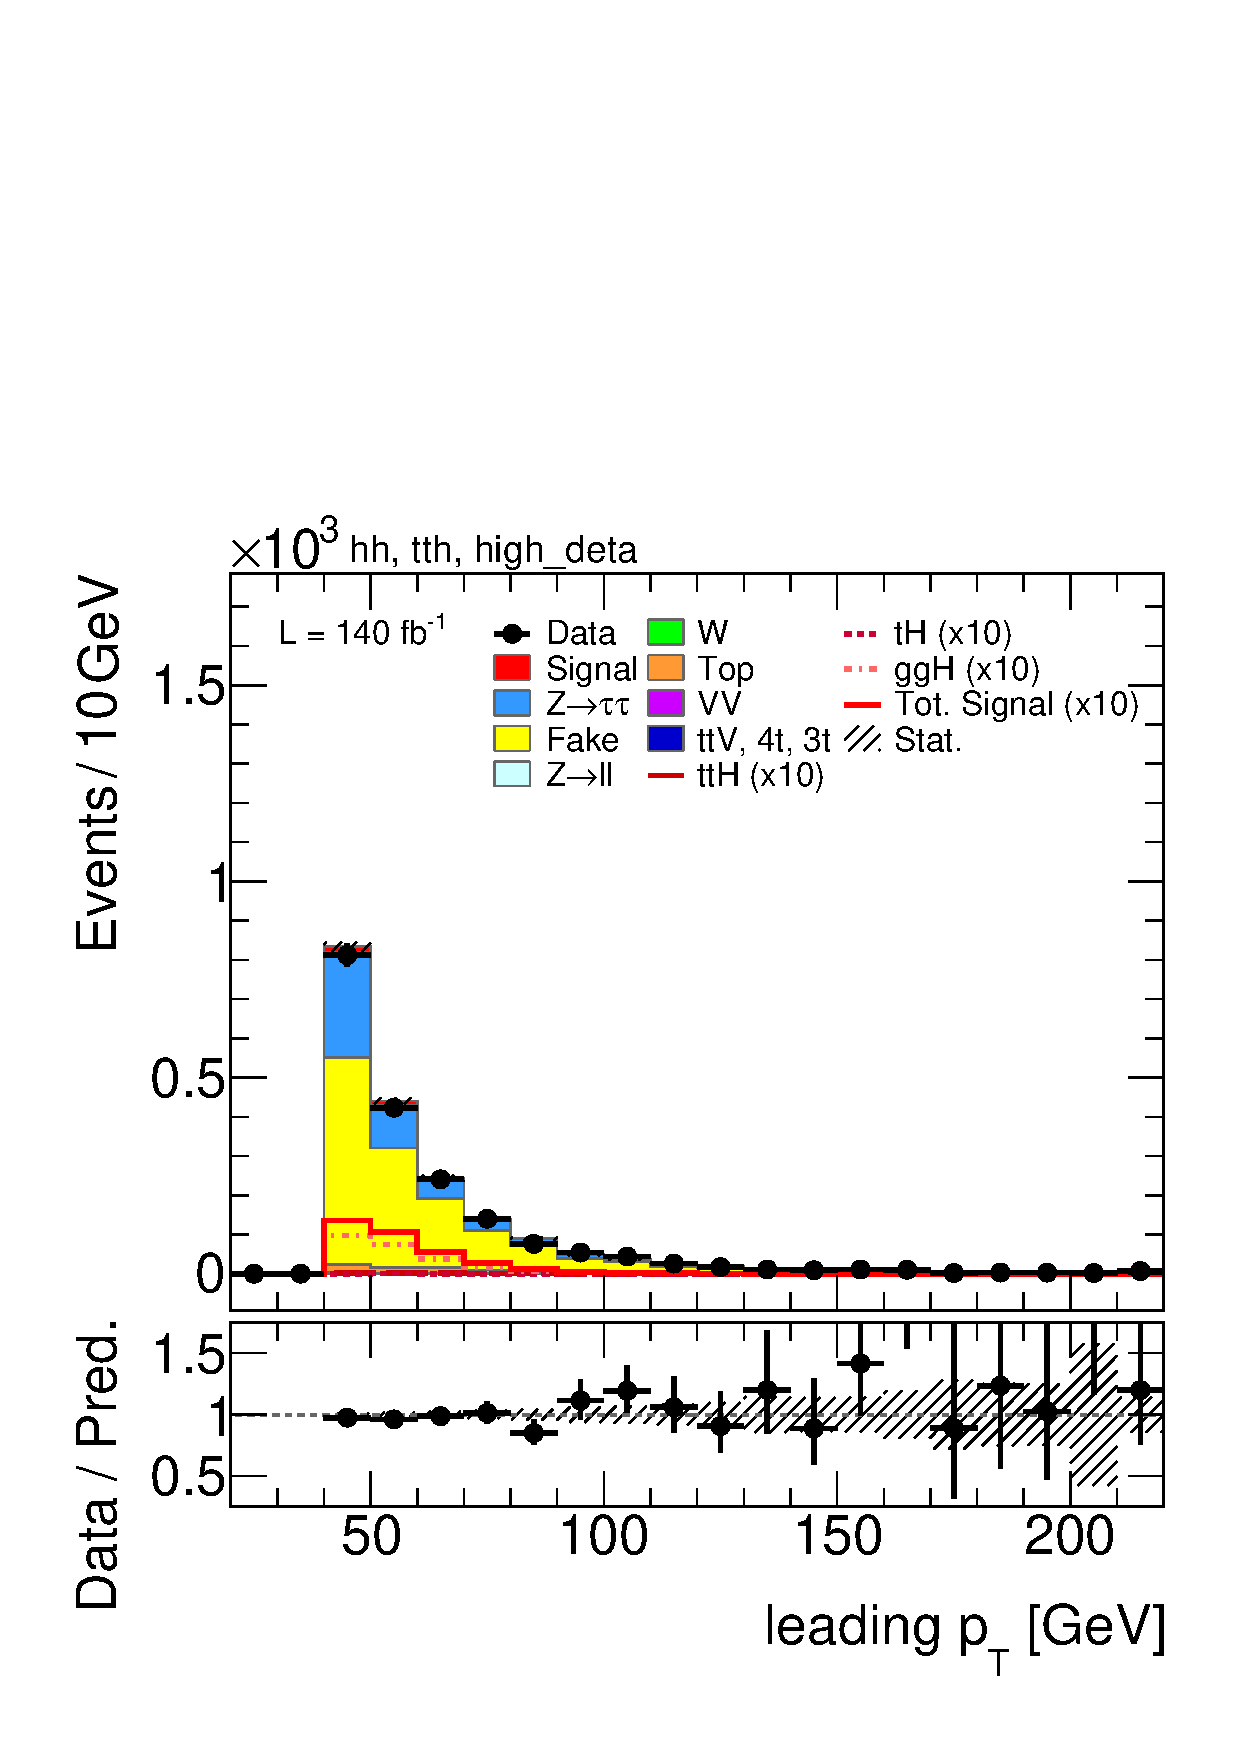
\includegraphics[width=\textwidth]{images/using_highdeta_ffs_run2_inclusive/plot_tau_0_pt_hh_tth_15_16_17_18_high_deta.pdf}
          \caption{}
        \end{subfigure}
        \hfill
        \begin{subfigure}[b]{0.45\textwidth}
          \centering
          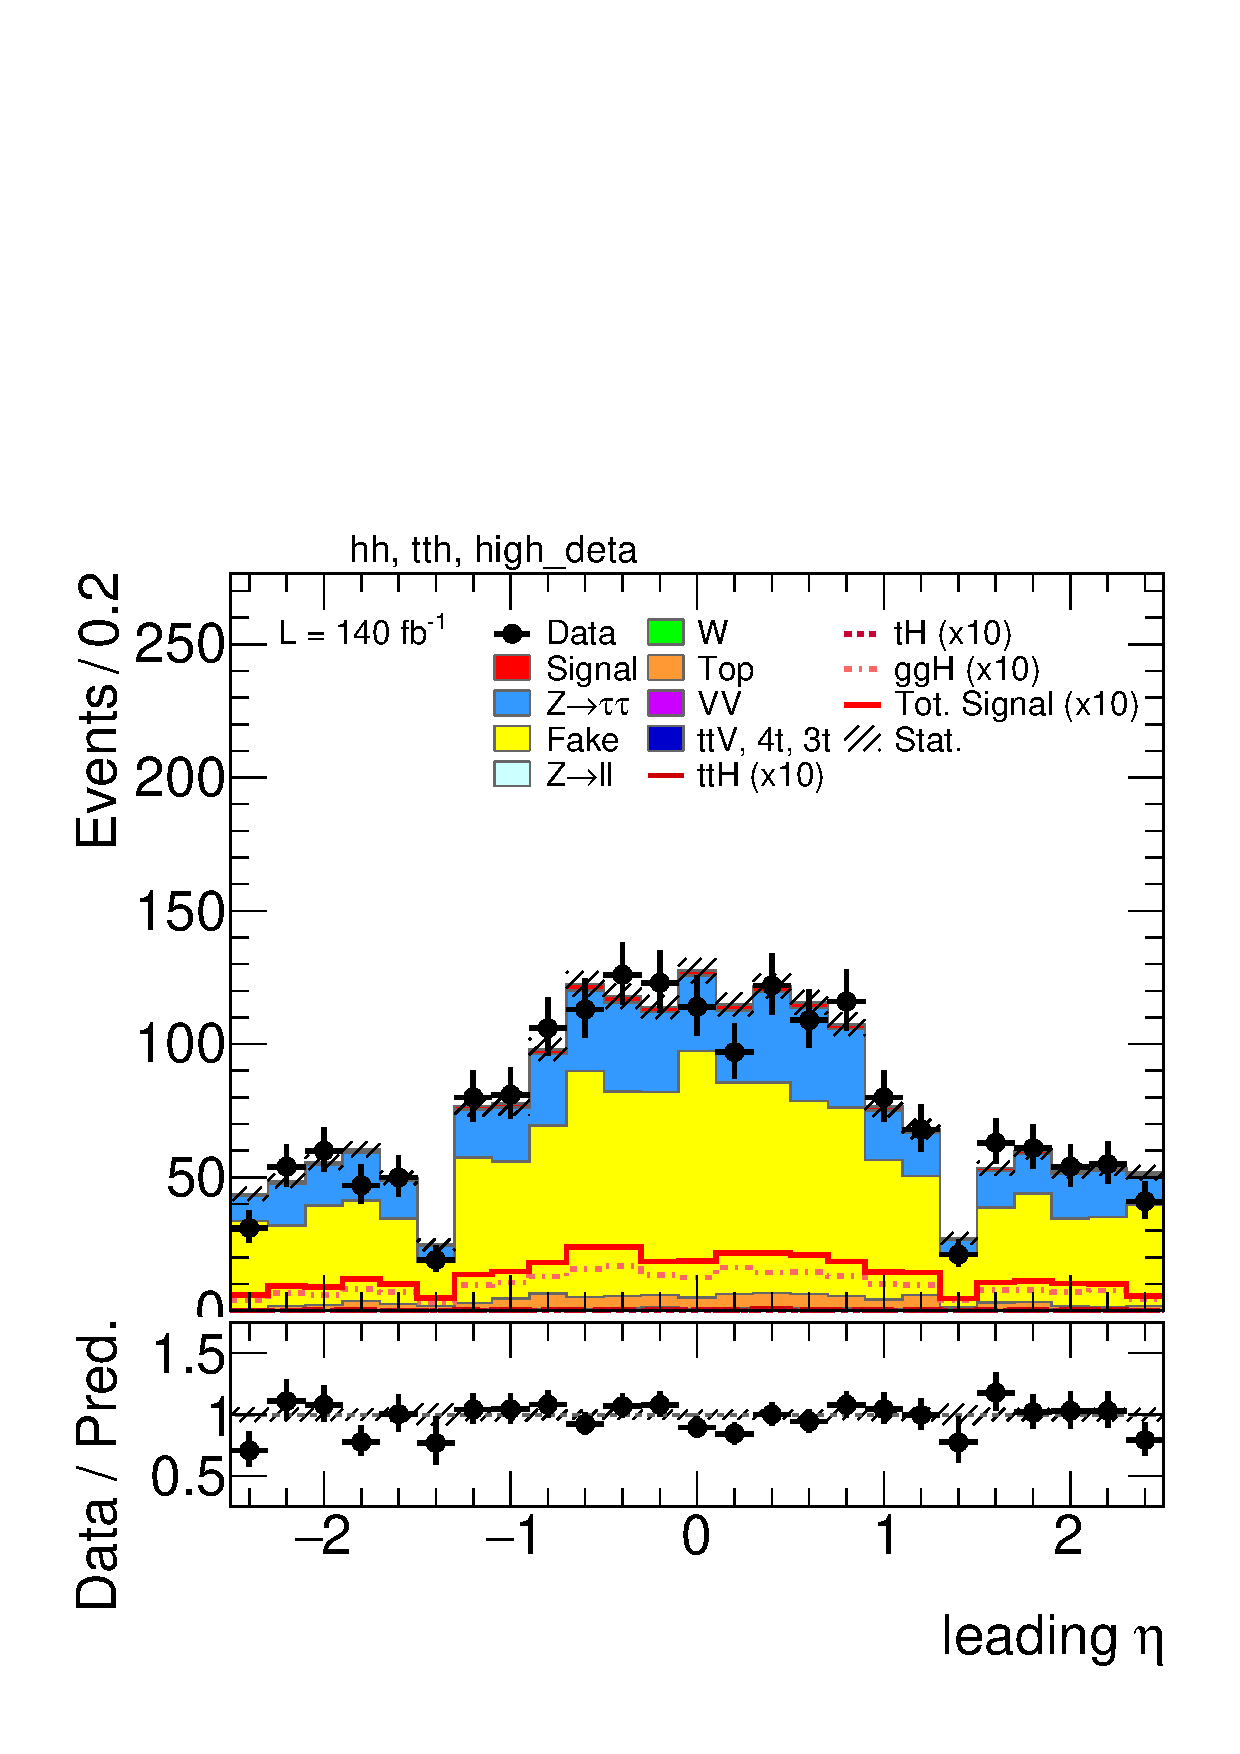
\includegraphics[width=\textwidth]{images/using_highdeta_ffs_run2_inclusive/plot_tau_0_eta_hh_tth_15_16_17_18_high_deta.pdf}
          \caption{}
        \end{subfigure}
    
        \begin{subfigure}[b]{0.45\textwidth}
          \centering
          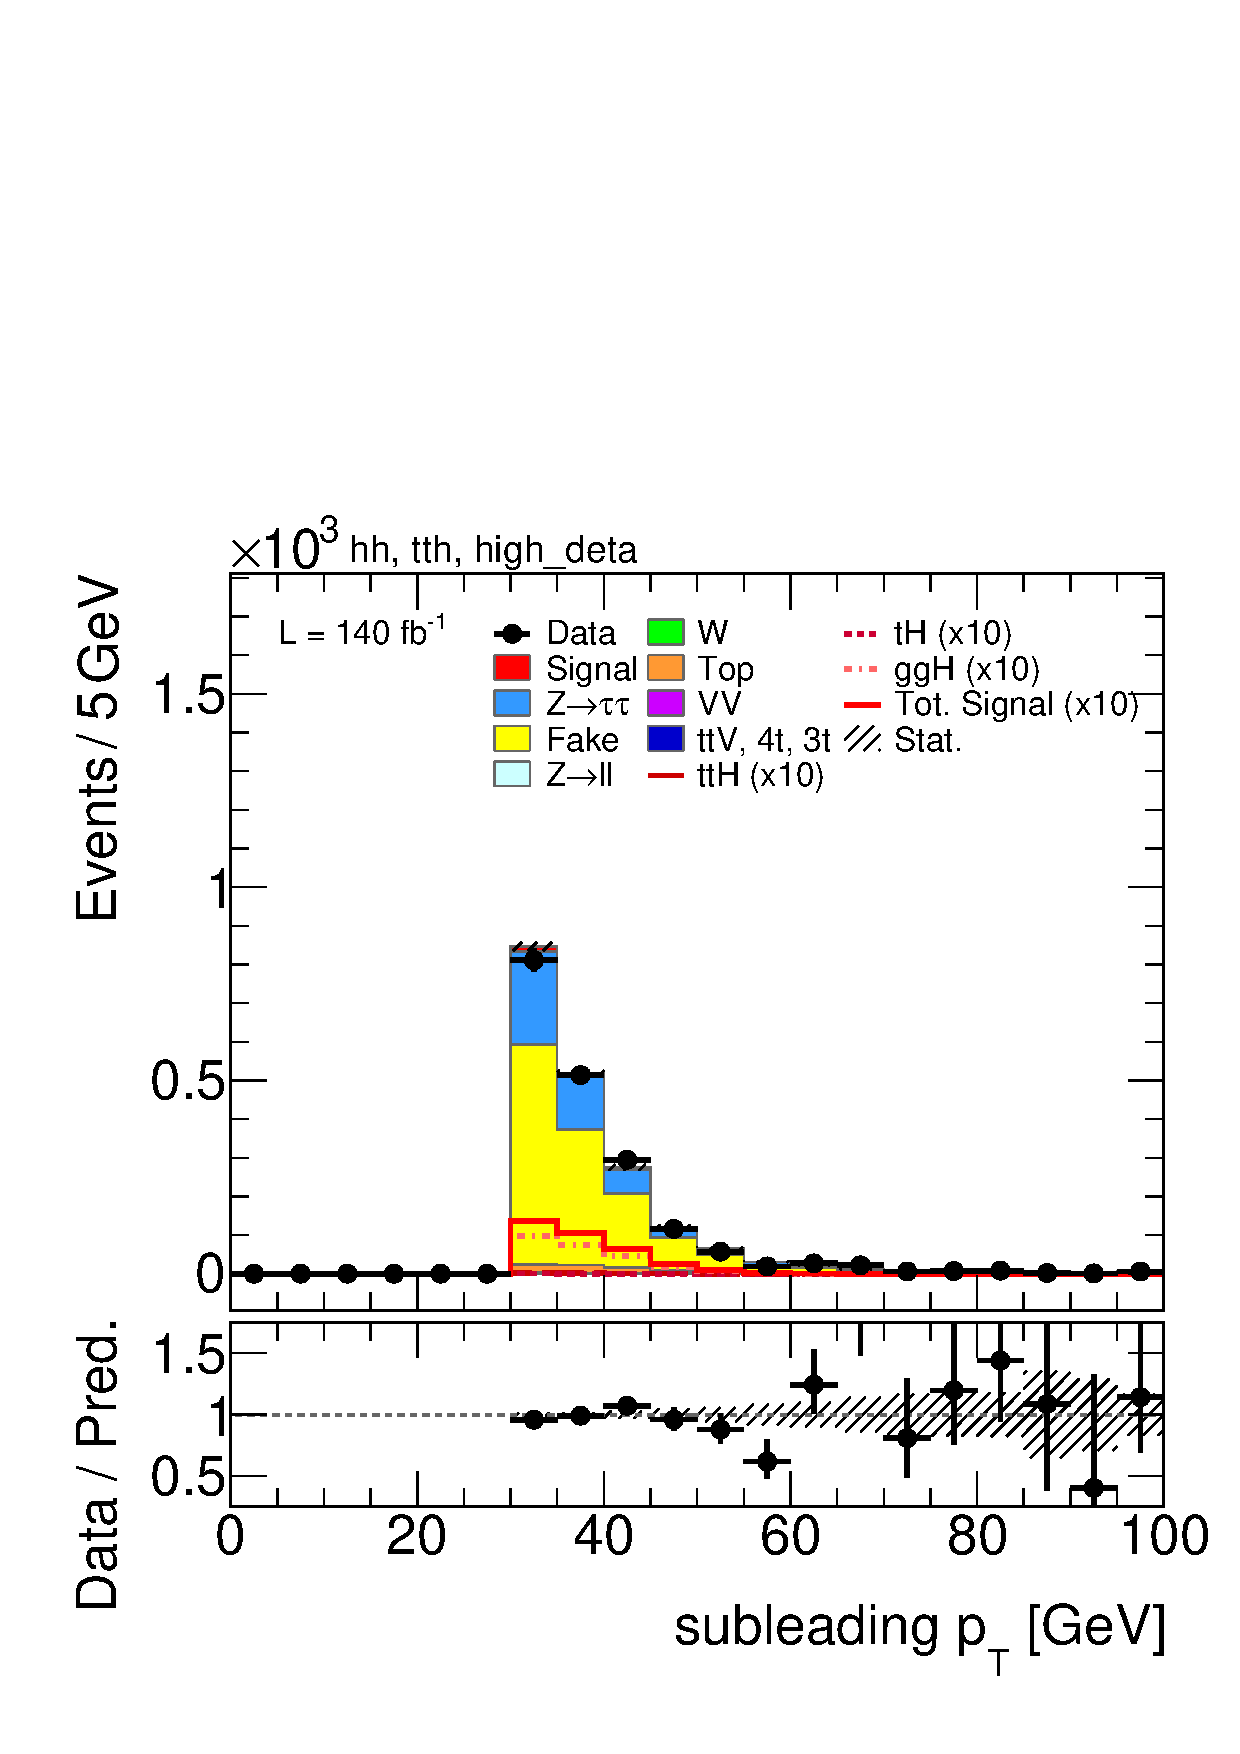
\includegraphics[width=\textwidth]{images/using_highdeta_ffs_run2_inclusive/plot_tau_1_pt_hh_tth_15_16_17_18_high_deta.pdf}
          \caption{}
        \end{subfigure}
        \hfill
        \begin{subfigure}[b]{0.45\textwidth}
          \centering
          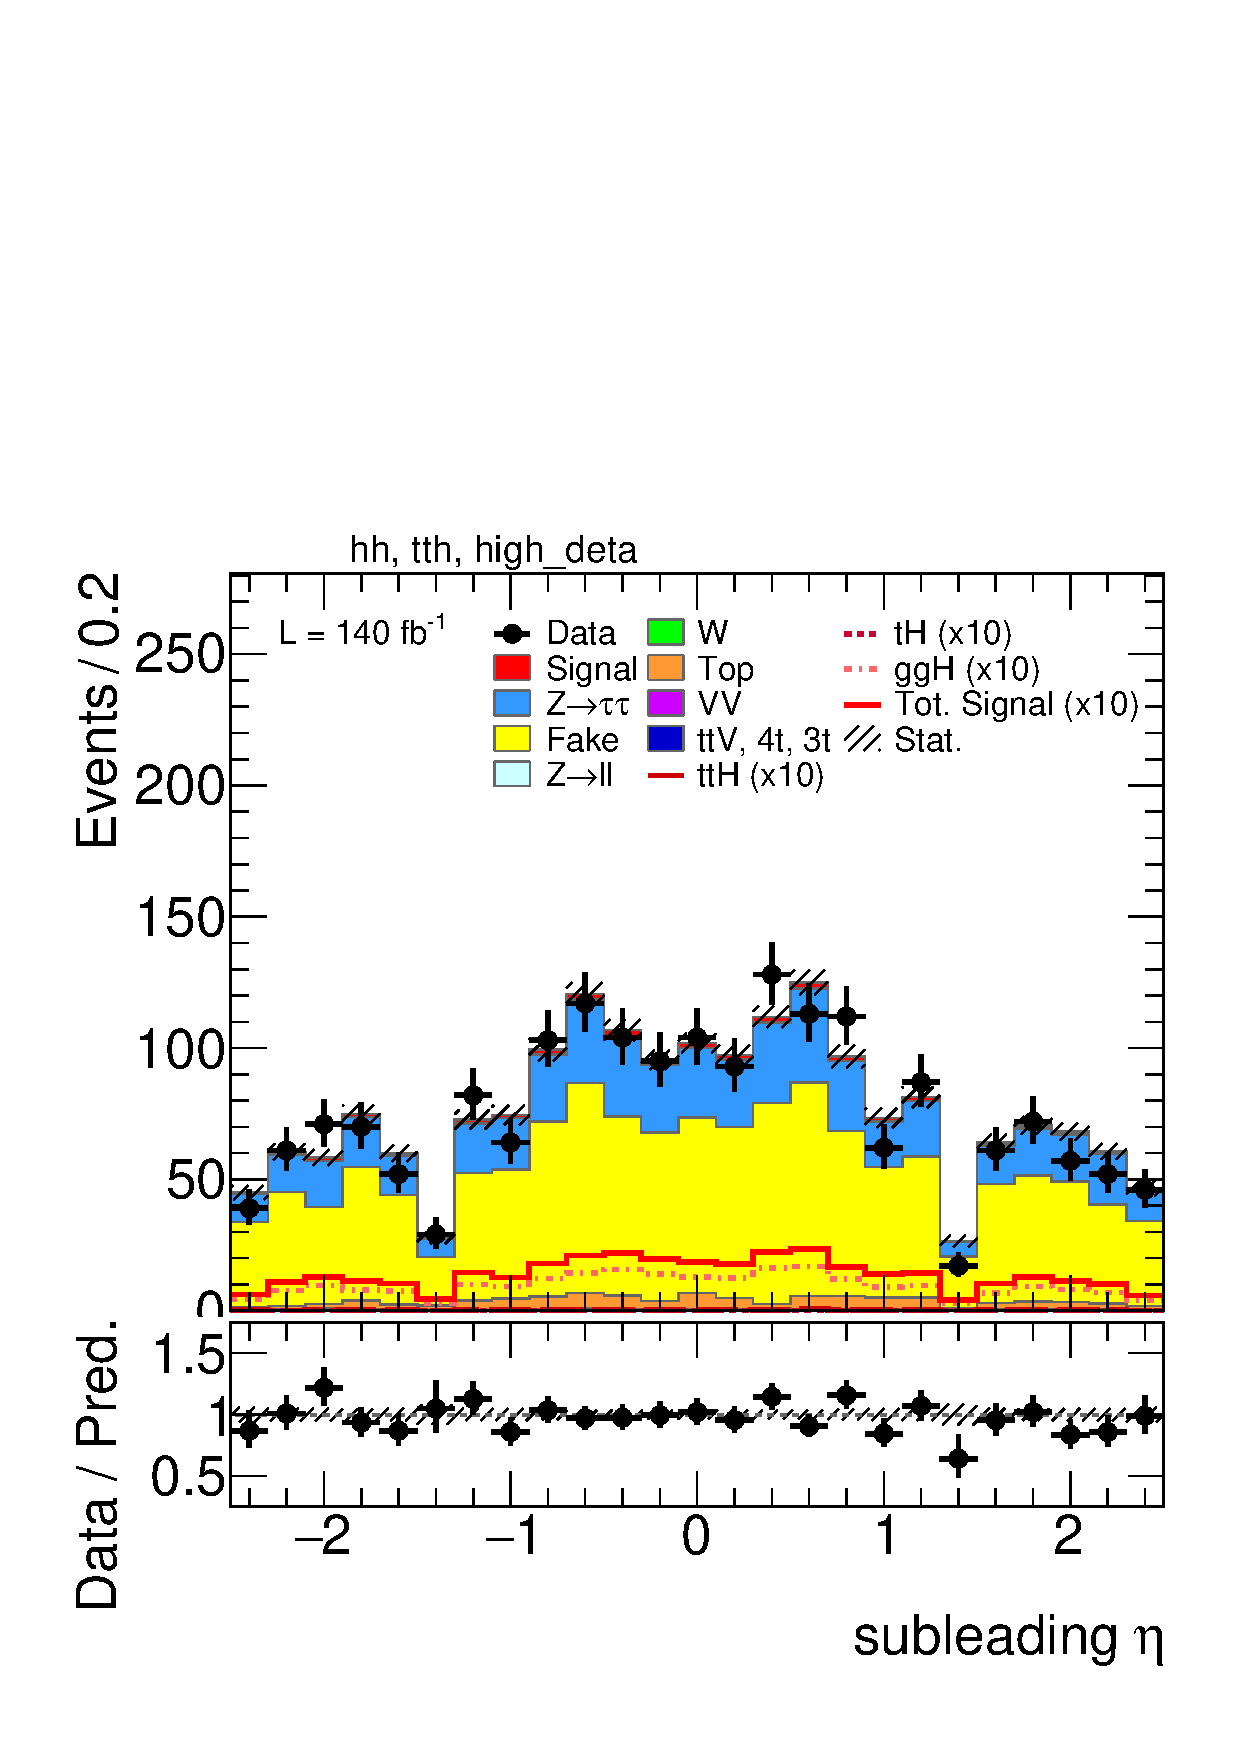
\includegraphics[width=\textwidth]{images/using_highdeta_ffs_run2_inclusive/plot_tau_1_eta_hh_tth_15_16_17_18_high_deta.pdf}
          \caption{}
        \end{subfigure}
        \caption{
    Closure and validation of the fake-\tauhad background estimated in Run-2 dataset with the alternative high-$\Delta \eta (\tau_0, \tau_1)$ \tauhadhad CR, evaluated in the high-$\Delta \eta (\tau_0, \tau_1)$ region at preselection level.
    The comparison is shown as a function of the \pt and $\eta$ of the leading (a), (b), and subleading (c), (d), \tauhad candidates. Only statistical uncertainties are included.
    Data are compared to the estimated fake-\tauhad background.
  }
  \label{fig:closure_validation_highdeta_run2}
\end{figure}

The remaining source of uncertainty in the estimation of this background is referred to as the parametrization uncertainty. Although it has only a minor impact on the analysis, it is re-derived by evaluating the effect of estimating the background contribution using FFs calculated separately for the leading and subleading \tauhad candidates in the \tauhadhad same-sign region, which then need to be combined, instead of relying on a single nominal fake factor extracted in the \taulephad $W$+jets control region.  

In this case, rather than considering the variation as the difference in the fake-\tauhad background contribution obtained with FFs derived either in the same-sign region or in the nominal control region, the approach is based on computing the Data/MC ratio from the distribution of the \mmc. The fake-\tauhad contribution in this distribution is estimated using the FFs derived in the \tauhadhad same-sign control region. This Data/MC ratio is then applied as a weight to the nominal fake-\tauhad background estimate in the analysis regions. The variation is taken as the difference between this weighted contribution, obtained in bins of \mmc, and the nominal prediction. More details about this procedure can be found in Ref.~\cite{serhat_tesis}.

  


\FloatBarrier
\section{New MVA strategy for event categorization}

The classification of events of interest within the defined phase space closely follows the approach discussed in Section~\ref{sec:tth_mva}. The same multiclass BDT algorithm is employed, but in this case it is extended to a total of four classes, including an additional one for the \thtt signal.

It should be emphasised that an inclusive training in \pth is carried out at this stage. The objective is not to perform a statistical fit targeting different STXS phase space bins in order to refine the precision of the measurements, but rather to obtain a combined study of \ttH and \thqb, with the aim of assessing the sensitivity for this newly incorporated production mode.

The BDT has been trained using together the available MC simulations for both signals, \ztautau and \ttbar, corresponding to the whole Run~2 data-taking period (at $\sqrt{s}=13$~TeV), and Run~3 (2022-2024, at $\sqrt{s} = 13.6$~TeV).
Despite the difference in the center-of-mass energy, the statistical power of combining both sets of MC samples improves the overall BDT performance.

\subsection{New 4-class BDT}
The same input variables previously used to separate \ttH from \ztautau and from \ttbar are also employed, since the features exploited to distinguish these processes are also expected to provide separation power for \thqb.
Nevertheless, in order to maximize the separation of \ttHtt and \thtt, a set of additional variables is incorporated. These new observables are primarily defined based on the properties of $b$-tagged jets ($b$-jets) and non-$b$-tagged jets (light jets) in the final state, or on features describing the $b$-jet pairs. Specifically, the added variables are the following:

\begin{itemize}
  \small
  \item \texttt{n\_ljets}: number of light (i.e., non-$b$-tagged) jets,
  \item \texttt{n\_ljets\_maxSameEta}: number of light jets with the same $\eta$ sign,
  \item \texttt{bjet\_0\_eta}: $\eta$ of the leading $b$-jet,
  \item \texttt{bjet\_0\_pt}: $p_{\mathrm{T}}$ of the leading $b$-jet,
  \item \texttt{dEta\_bH\_max}: maximum $\Delta \eta$ between the visible decay products of the Higgs boson and any $b$-jet,
  \item \texttt{n\_bjets\_GN2v01\_FixedCutBEff\_70}: $b$-jets multiplicity,
  \item \texttt{dEta\_lb\_max}: largest $\Delta \eta$ between any light jet and $b$-jet pair,
  \item \texttt{m\_ll\_max}: largest invariant mass of any pair of light jets in the final state.
\end{itemize}

These variables are designed to exploit differences in the origin of jets and $b$-jets in the considered processes.
For instance, the leading jet in \thqb is often significantly more forward compared to the remaining jets in its final state or to those in \ttH. In addition, in \thqb there exists a leading $b$-jet produced directly from one of the initial-state partons, rather than from the decay of a top quark, either the singly produced one in \thqb or one of the top quarks in \ttH.

This feature is exploited through the study of the $\eta$ and $p_{\mathrm{T}}$ of the leading $b$-jet, as well as its relation to the Higgs boson or to other light jets. The additional $b$-jet in \thqb is typically less energetic and exhibits a broader $\eta$ distribution, and it is not correlated with either the Higgs boson or the top quark. In contrast, the $b$-jets in \ttH are generally more central and have larger transverse momentum, similarly to the $b$-jet produced from the top quark in \thqb.

The invariant mass of the two light jets with the largest separation can also be highly discriminating, particularly in \thqb, where the spectator jet previously discussed tends to carry substantial energy. Additional jet-related properties, such as the $\eta$ of the five leading jets or the ratios of their transverse momenta, were already included in the previous analysis for the separation from \ztautau, but they also prove to be highly valuable in this context.

In Figures~\ref{fig:th_vs_tth_1} and~\ref{fig:th_vs_tth_2}, the distributions of these new variables are shown for simulated \thqb and \ttH events, after applying the preselection cuts used in the training of the BDT.

% =========================
% Primera figura (4 vars)
% =========================
\begin{figure}[htbp]
  \centering
  % 1a fila
  \begin{subfigure}[b]{0.45\textwidth}
    \centering
    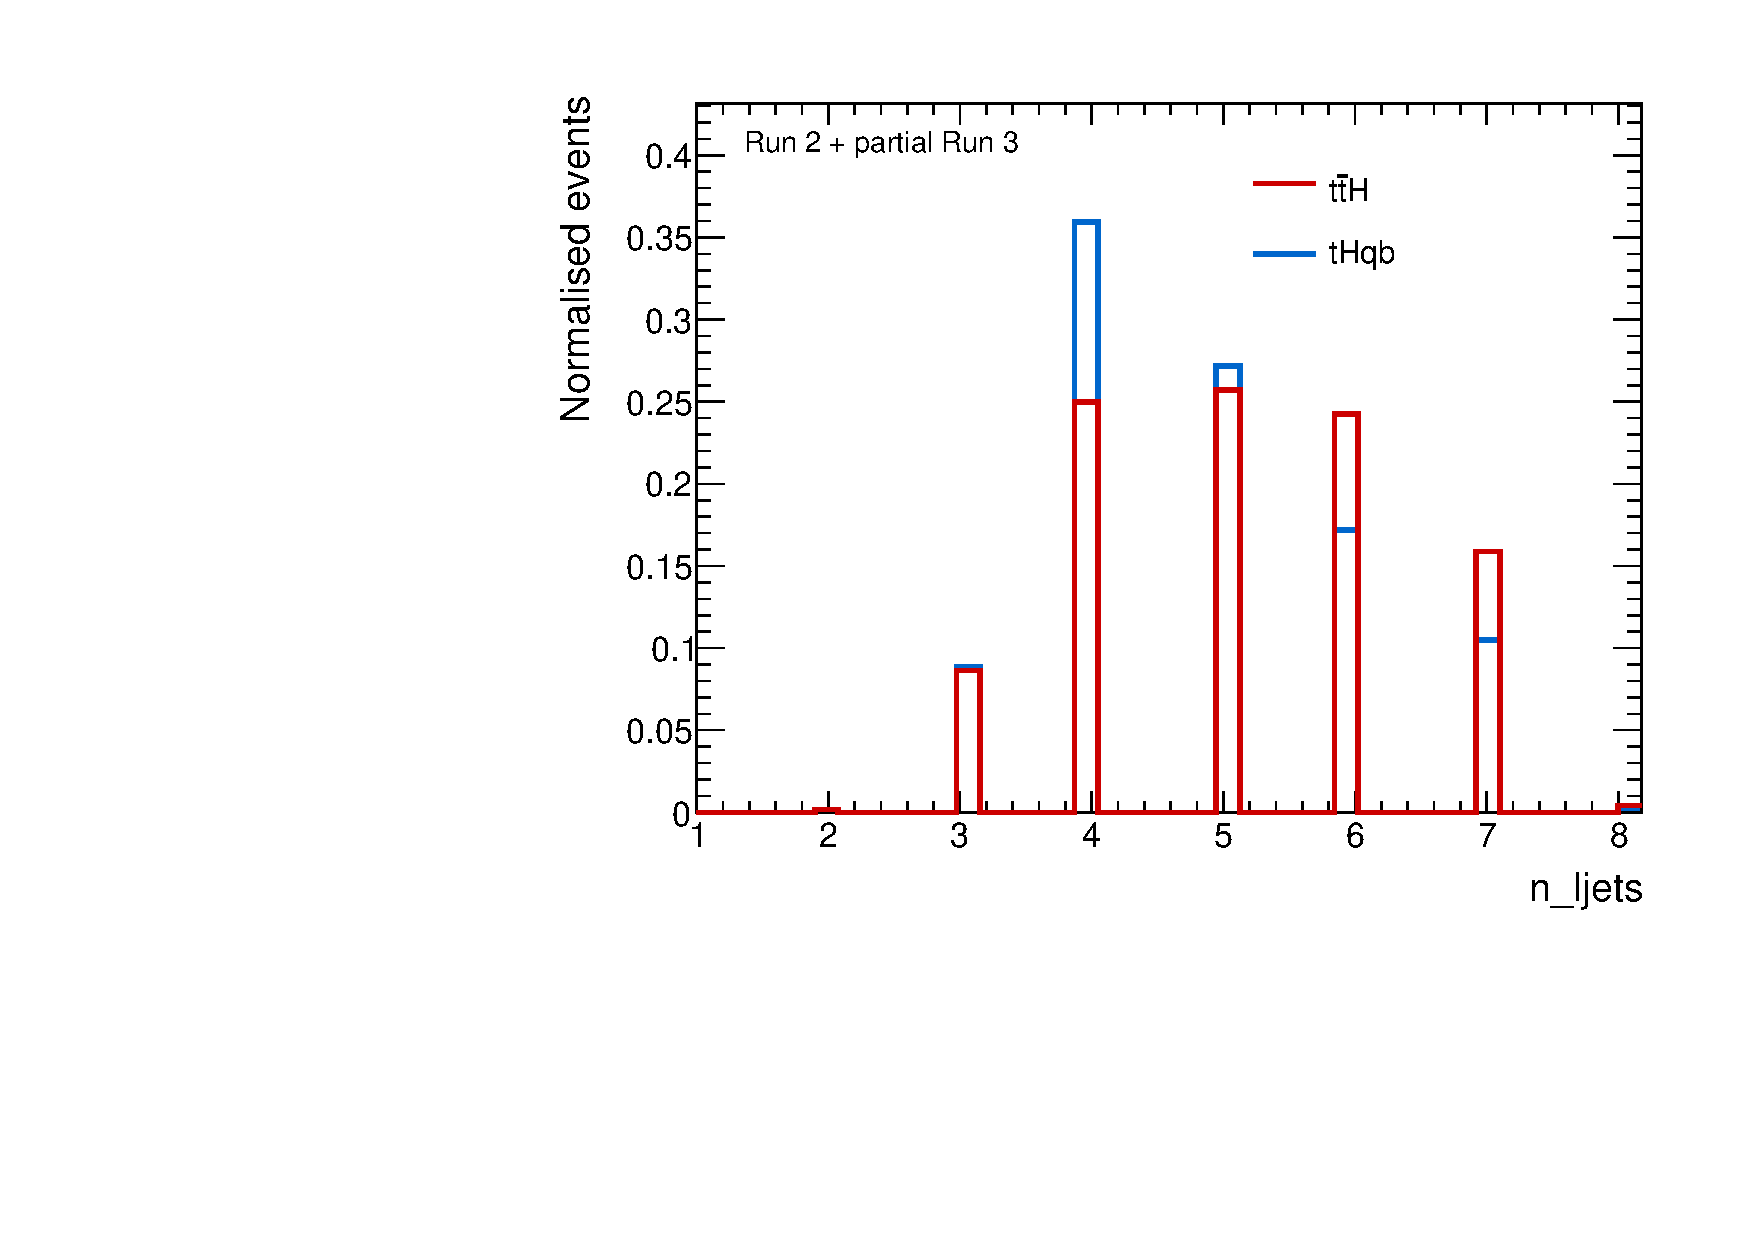
\includegraphics[width=\textwidth]{images/plots_tH_tHqb_for_thesis/n_ljets_signals_ATLAS.pdf}
    \caption{$n_{\text{ljets}}$}
    \label{fig:n_ljets}
  \end{subfigure}
  \hfill
  \begin{subfigure}[b]{0.45\textwidth}
    \centering
    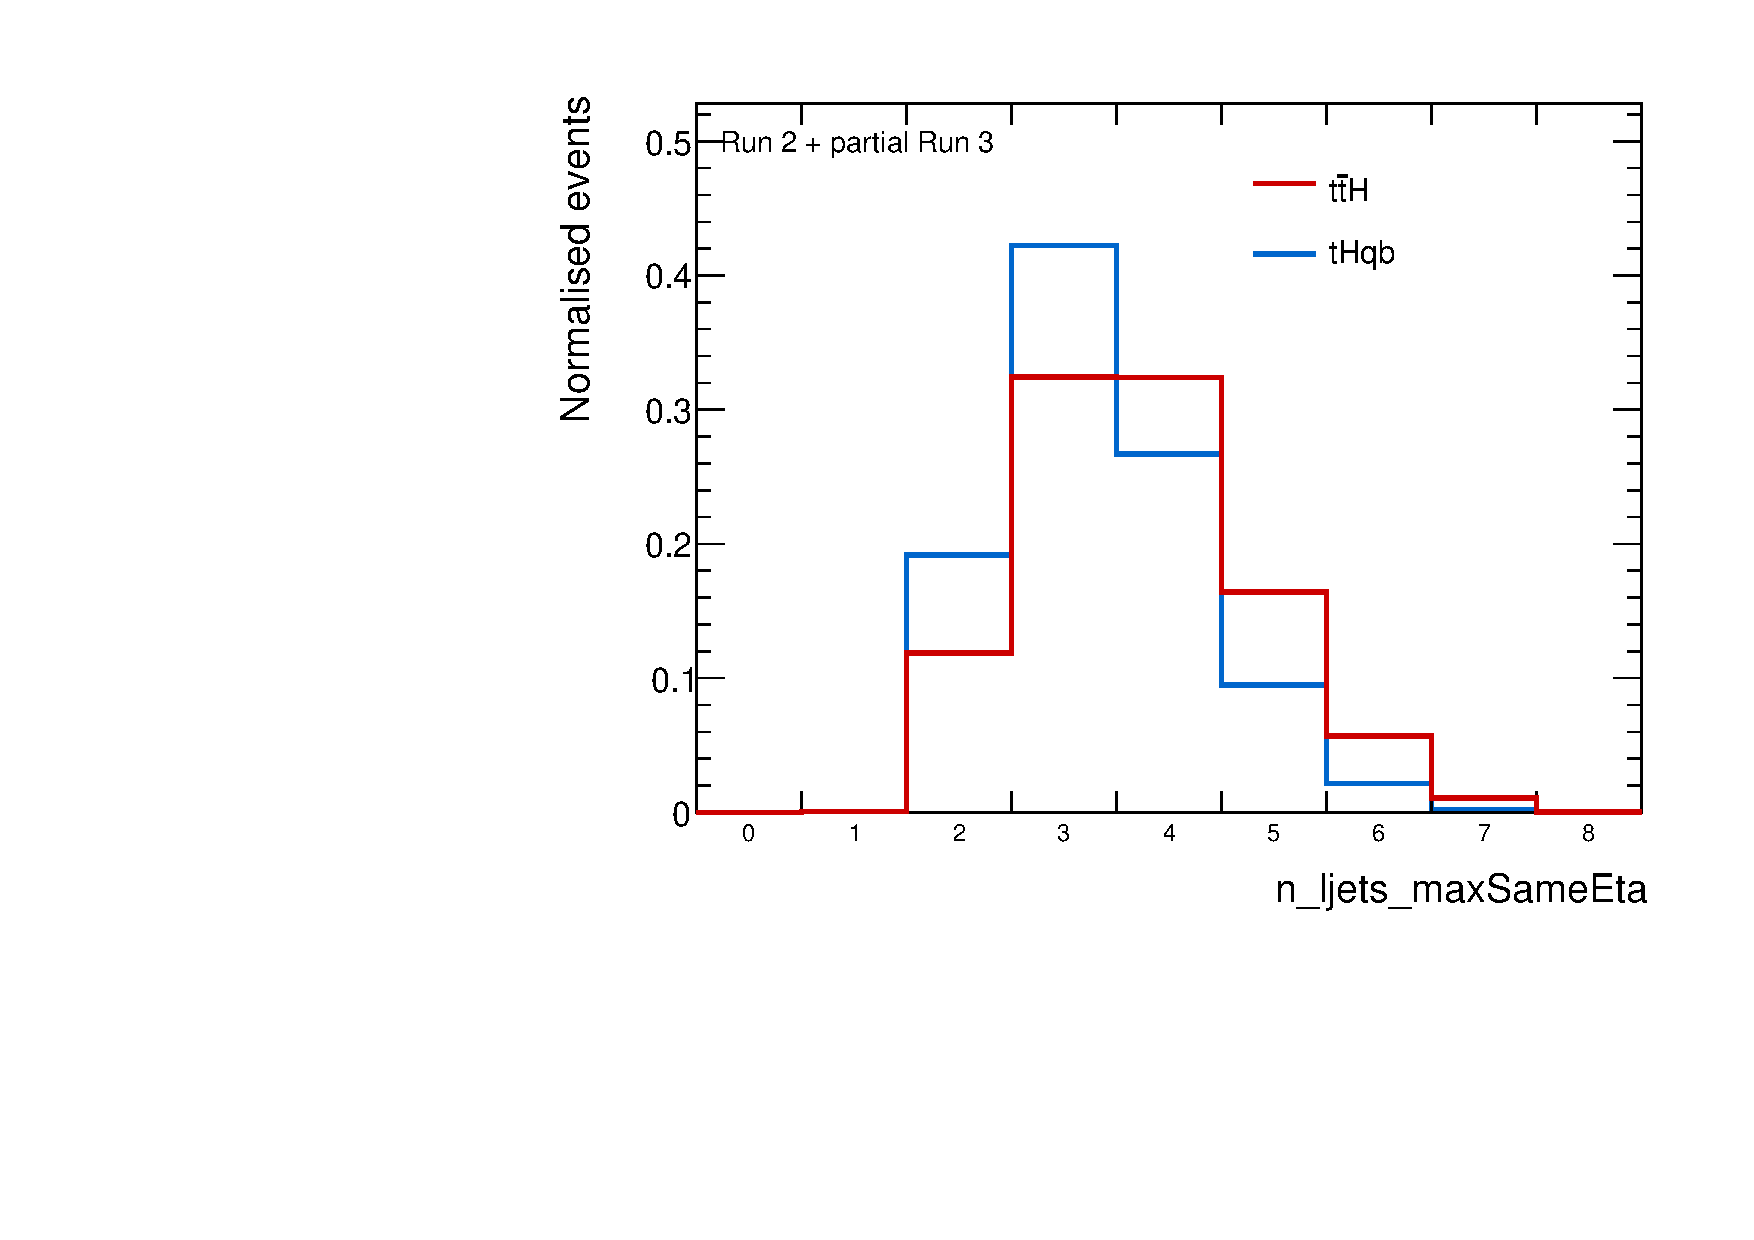
\includegraphics[width=\textwidth]{images/plots_tH_tHqb_for_thesis/n_ljets_maxSameEta_signals_ATLAS.pdf}
    \caption{$n_{\text{ljets}}^{\text{same }\eta}$}
    \label{fig:n_ljets_maxSameEta}
  \end{subfigure}

  % 2a fila
  \vskip\baselineskip
  \begin{subfigure}[b]{0.45\textwidth}
    \centering
    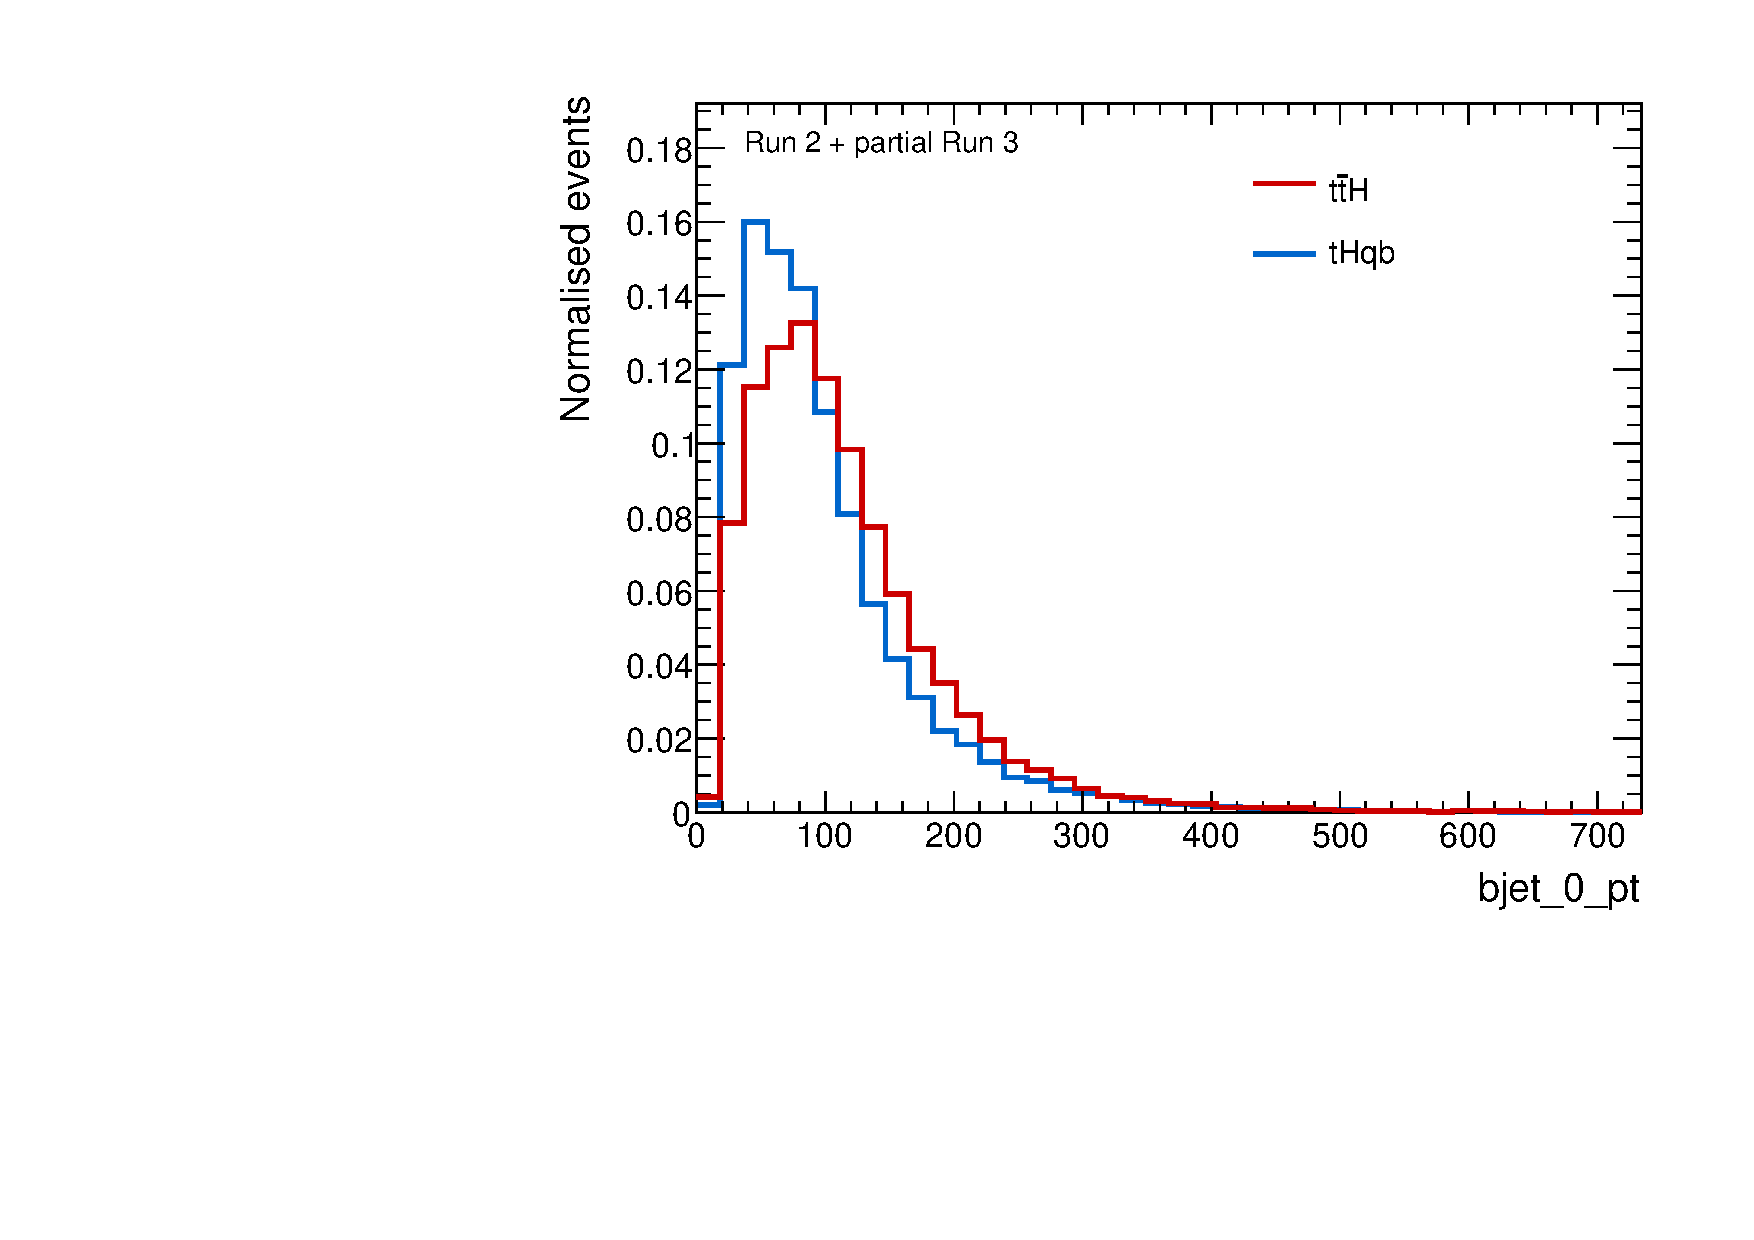
\includegraphics[width=\textwidth]{images/plots_tH_tHqb_for_thesis/bjet_0_pt_signals_ATLAS.pdf}
    \caption{$\eta$ of the leading $b$-jet}
    \label{fig:bjet0_eta}
  \end{subfigure}
  \hfill
  \begin{subfigure}[b]{0.45\textwidth}
    \centering
    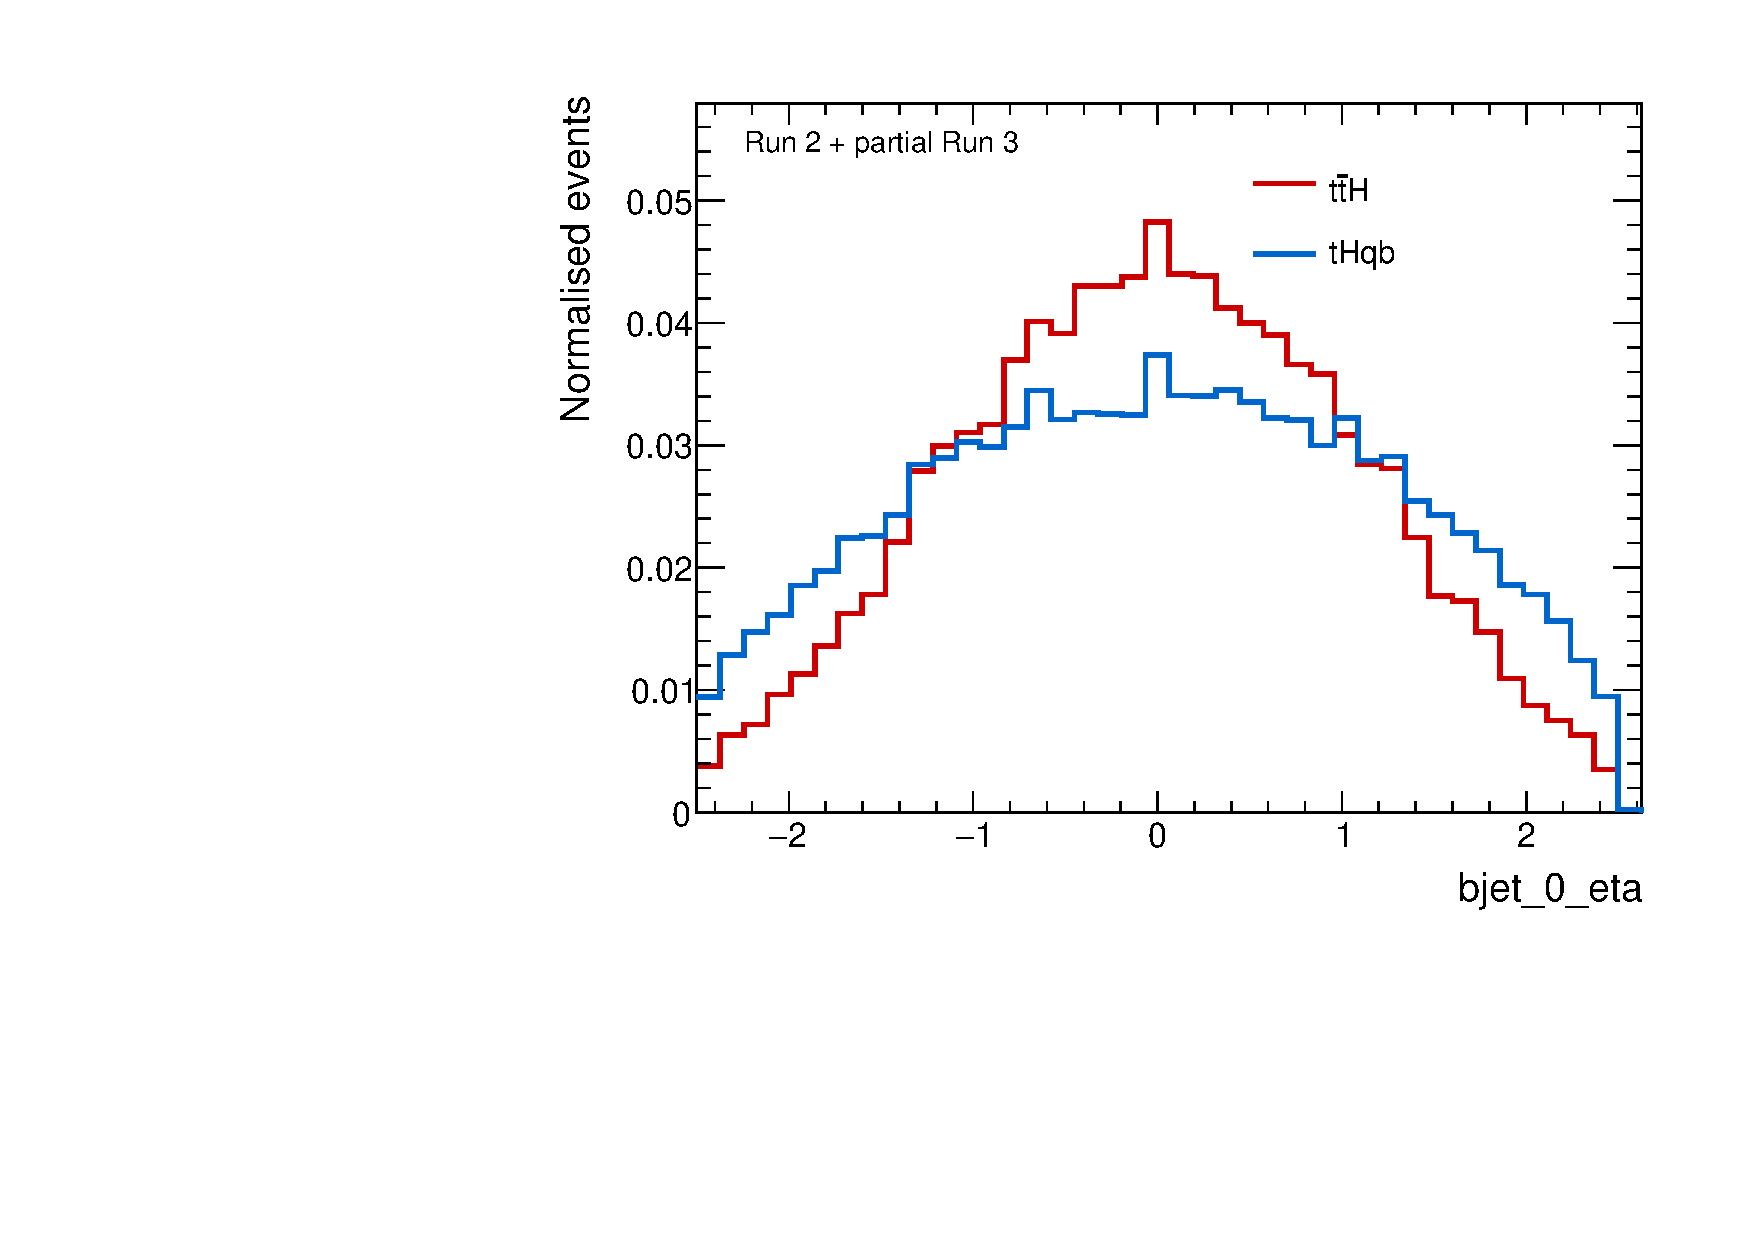
\includegraphics[width=\textwidth]{images/plots_tH_tHqb_for_thesis/bjet_0_eta_signals_ATLAS.pdf}
    \caption{$p_{\mathrm{T}}$ of the leading $b$-jet}
    \label{fig:bjet0_pt}
  \end{subfigure}

  \caption{Distributions of additional input variables used in the BDT training, shown for simulated \thqb and \ttH events after preselection cuts. 
  The observables exploit differences in the origin and kinematics of jets and $b$-jets in the two processes. 
  }
  \label{fig:th_vs_tth_1}
\end{figure}


% =========================
% Segunda figura (4 vars)
% =========================
\begin{figure}[htbp]
  \centering
  % 1a fila
  \begin{subfigure}[b]{0.45\textwidth}
    \centering
    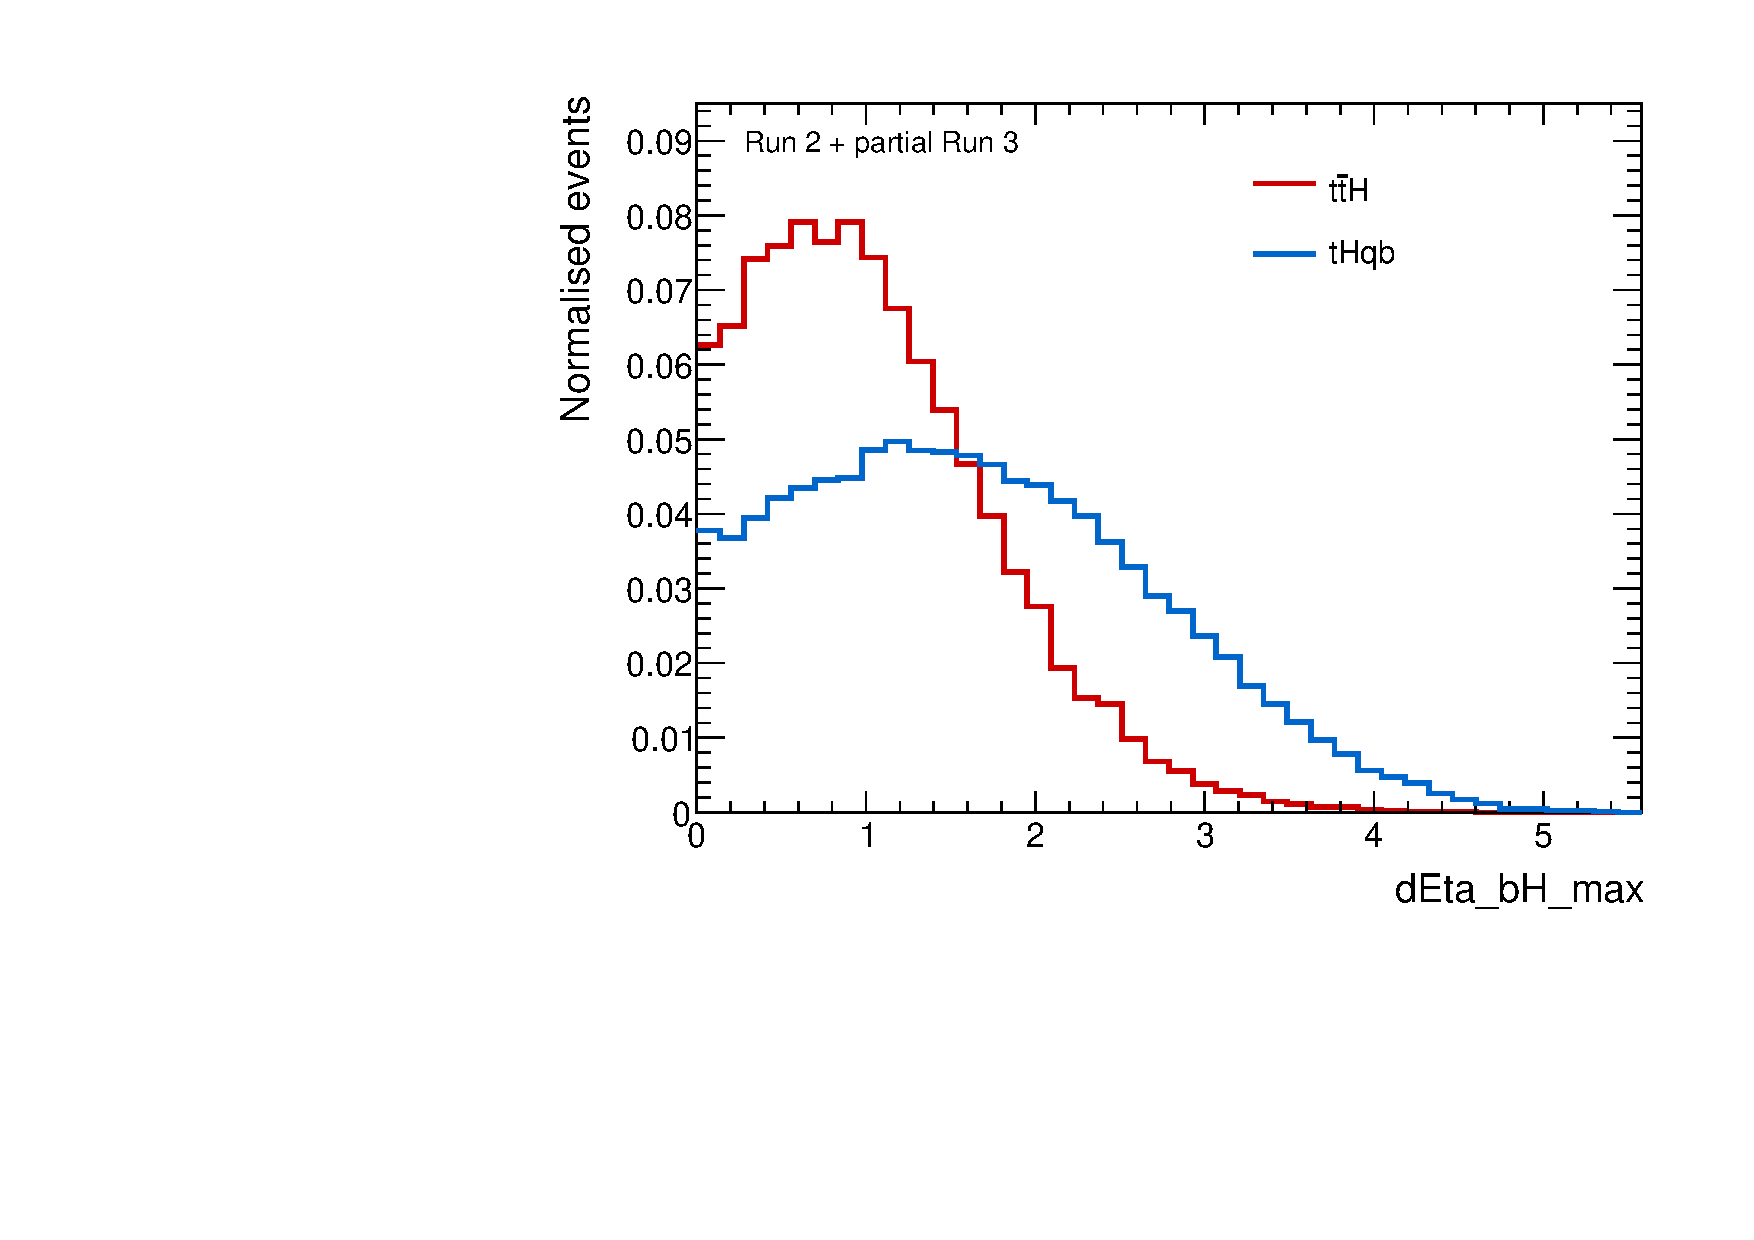
\includegraphics[width=\textwidth]{images/plots_tH_tHqb_for_thesis/dEta_bH_max_signals_ATLAS.pdf}
    \caption{Max.\ $\Delta \eta (H,b\text{jet})$}
    \label{fig:dEta_bH_max}
  \end{subfigure}
  \hfill
  \begin{subfigure}[b]{0.45\textwidth}
    \centering
    \includegraphics[width=\textwidth]{images/plots_tH_tHqb_for_thesis/n_bjets_GN2v01_FixedCutBEff_70_signals_ATLAS.pdf}
    \caption{$b$-jet multiplicity}
    \label{fig:n_bjets}
  \end{subfigure}

  % 2a fila
  \vskip\baselineskip
  \begin{subfigure}[b]{0.45\textwidth}
    \centering
    \includegraphics[width=\textwidth]{images/plots_tH_tHqb_for_thesis/dEta_lb_max_signals_ATLAS.pdf}
    \caption{Max.\ $\Delta \eta (l\text{jet},b-\text{jet})$}
    \label{fig:dEta_lb_max}
  \end{subfigure}
  \hfill
  \begin{subfigure}[b]{0.45\textwidth}
    \centering
    \includegraphics[width=\textwidth]{images/plots_tH_tHqb_for_thesis/m_ll_max_signals_ATLAS.pdf}
    \caption{Largest invariant mass of two light jets}
    \label{fig:m_ll_max}
  \end{subfigure}

  \caption{Distributions of additional input variables used in the BDT training, shown for simulated \thqb and \ttH events after preselection cuts. 
  The observables exploit differences in the origin and kinematics of jets and $b$-jets in the two processes. 
  }
  \label{fig:th_vs_tth_2}
\end{figure}

Finally, in Table~\ref{tab:all_vars} the complete list of 29 input variables is presented and Figures~\ref{th_tth_vars_tmva_1}-\ref{th_tth_vars_tmva_3} show, analogously to what was presented in Section~\ref{sec:tth_mva}, the distributions of all of them employed in this new training for the four event classes under consideration.

\begin{table}[htbp]
  \small
  \centering
  \caption{Variables used in the multivariate tagger. Additional variables introduced in the current training for discriminating between $t\bar{t}H$ and $tHqb$ are shown in bold.}
  \renewcommand{\arraystretch}{1.3}
  \setlength{\tabcolsep}{10pt}
  \begin{tabular}{p{2.2cm} p{10.5cm}}
    \toprule
    \textbf{Group} & \textbf{Variable} \\
    \midrule

    \multirow{9}{*}{\rotatebox{90}{Jet properties}} 
    & Invariant mass of the two leading jets $p_{\text{T}}(jj)$ \\
    & Product of $\eta$ of the two leading jets \\
    & Sub-leading jet $p_{\text{T}}$ \\
    & $\eta$ of the 5 leading jets \\
    & Scalar sum of all jets $p_{\text{T}}$ \\
    & Scalar sum of all $b$-tagged jets $p_{\text{T}}$ \\
    & Best $W$-candidate dijet invariant mass \\
    & Best top-quark-candidate three-jet invariant mass \\
    & Ratio of the $p_{\text{T}}$ of jet pairs \\
    \midrule

    \multirow{6}{*}{\rotatebox{90}{Angular distances}} 
    & $\Delta\phi$ between the two leading jets \\
    & $\Delta\eta$ between the two leading jets \\
    & Minimum $\Delta R$ between two jets \\
    & Minimum $\Delta R$ between a $b$-tagged jet and a $\tau$ \\
    & $|\Delta\eta(\tau,\tau)|$ \\
    & $\Delta R(\tau,\tau)$ \\
    \midrule

    \multirow{3}{*}{\rotatebox{90}{$\tau$-lepton}} 
    & $p_{\text{T}}(\tau)$ \\
    & Sub-leading $\tau$ $p_{\text{T}}$ \\
    & Leading $\tau$ $\eta$ \\
    \midrule

    \multirow{2}{*}{\rotatebox{90}{\etmiss}} 
    & Missing transverse momentum $E_{T}^{\text{miss}}$ \\
    & Smallest $\Delta\phi(\tau, \vec{E}_{T}^{\text{miss}})$ \\
    \midrule

    \multirow{8}{*}{\rotatebox{90}{$t\bar{t}H$ vs.\ $tHqb$}} 
    & \textbf{Number of light (non-$b$-tagged) jets} \\
    & \textbf{Number of light jets with the same $\eta$ sign} \\
    & \textbf{$b$-jets multiplicity} \\
    & \textbf{$\eta$ of the leading $b$-jet} \\
    & \textbf{$p_{\text{T}}$ of the leading $b$-jet}  \\
    & \textbf{Largest $\Delta \eta$ between any light-jet and $b$-jet pair}  \\
    & \textbf{Maximum $\Delta \eta$ between the visible Higgs decay products and any $b$-jet}  \\
    & \textbf{Largest invariant mass of any pair of light jets}  \\
    \bottomrule
  \end{tabular}
  \label{tab:all_vars}
\end{table}

\begin{figure}[htbp]
  \centering
  % Primera figura
  \begin{subfigure}{0.95\linewidth}
    \centering
    \includegraphics[width=\linewidth]{images/plots_tH_tHqb_for_thesis/variables_id_c1.png}
  \end{subfigure}
  \vspace{0.5cm} % Espacio vertical entre las dos
  % Segunda figura
  \begin{subfigure}{0.95\linewidth}
    \centering
    \includegraphics[width=\linewidth]{images/plots_tH_tHqb_for_thesis/variables_id_c2.png}
  \end{subfigure}
  \caption{Distribution of the input variables used for the multiclass BDT training for \thtt + \ttHtt, evaluated on \ttHtt (blue), \thtt (red), \ztautau background (green) and \ttbar background (magenta).}
  \label{th_tth_vars_tmva_1}
  \end{figure}

  \begin{figure}[htbp]
    \centering
  % Segunda figura
  \begin{subfigure}{0.95\linewidth}
    \centering
    \includegraphics[width=\linewidth]{images/plots_tH_tHqb_for_thesis/variables_id_c3.png}
  \end{subfigure}
  \vspace{0.5cm} % Espacio vertical entre las dos
  % Segunda figura
  \begin{subfigure}{0.95\linewidth}
    \centering
    \includegraphics[width=\linewidth]{images/plots_tH_tHqb_for_thesis/variables_id_c4.png}
  \end{subfigure}
  \vspace{0.5cm} % Espacio vertical entre las dos
  % Segunda figura
  \caption{Distribution of the input variables used for the multiclass BDT training for \thtt + \ttHtt, evaluated on \ttHtt (blue), \thtt (red), \ztautau background (green) and \ttbar background (magenta).}
  \label{th_tth_vars_tmva_2}
  \end{figure}

  \begin{figure}[htbp]
    \centering
    \includegraphics[width=0.95\linewidth]{images/plots_tH_tHqb_for_thesis/variables_id_c5.png}
    \caption{Distribution of the input variables used for the multiclass BDT training for \thtt + \ttHtt, evaluated on \ttHtt (blue), \thtt (red), \ztautau background (green) and \ttbar background (magenta).}
    \label{th_tth_vars_tmva_3}
\end{figure}

It is worth noting that in this case the \mmc is included as an input variable in the BDT training. The reasons behind this choice will be discussed later in Section~\ref{new_categorization}.
\FloatBarrier
%%%%%%%%%%%%%%%%%%%%%%%%%%%%%%%%%%%%%%%%%%%%%%%%%%%%%%%%%%%%%%%%%%%%%%%%%%%%%%%%%%%%%%%%%%%%%%%%%%%
\subsubsection*{Data-MC modelling}
%%%%%%%%%%%%%%%%%%%%%%%%%%%%%%%%%%%%%%%%%%%%%%%%%%%%%%%%%%%%%%%%%%%%%%%%%%%%%%%%%%%%%%%%%%%%%%%%%%%

The MC modelling of the BDT input variables is checked with real collision data, especially after the modification in the event selection, MC samples and the addition of Run-3 data.

Figures~\ref{tth_vars_modelling_run3_1}–\ref{tth_vars_modelling_run3_3} show the agreement between data and MC in Run-3 datasets observed for the input variables, by comparing their distributions across all relevant processes at the preselection level. Analogously, Figures~\ref{tth_vars_modelling_run2_1}-\ref{tth_vars_modelling_run2_3} present also a correct agreement between data and MC for Run-2 datasets (without the application of any scaling factor).

\begin{figure}[htbp]
  \centering
  % Ajusta el espacio horizontal entre paneles (columna a columna)
  \setlength{\tabcolsep}{1.5pt}
  \renewcommand{\arraystretch}{0}

  \begin{tabular}{@{}c c c@{}}
    \includegraphics[width=0.33\textwidth]{images/plots_modelling_run2_run3_variables/run_3_tth/plot_ditau_dr_hh_tth_22_23_24.pdf} &
    \includegraphics[width=0.33\textwidth]{images/plots_modelling_run2_run3_variables/run_3_tth/plot_ditau_deta_hh_tth_22_23_24.pdf} &
    \includegraphics[width=0.33\textwidth]{images/plots_modelling_run2_run3_variables/run_3_tth/plot_met_reco_et_hh_tth_22_23_24.pdf} \\[4pt]
    \includegraphics[width=0.33\textwidth]{images/plots_modelling_run2_run3_variables/run_3_tth/plot_mWbest_hh_tth_22_23_24.pdf} &
    \includegraphics[width=0.33\textwidth]{images/plots_modelling_run2_run3_variables/run_3_tth/plot_SumPtBjet_hh_tth_22_23_24.pdf} &
    \includegraphics[width=0.33\textwidth]{images/plots_modelling_run2_run3_variables/run_3_tth/plot_mTopWbest_hh_tth_22_23_24.pdf} \\[4pt]
    \includegraphics[width=0.33\textwidth]{images/plots_modelling_run2_run3_variables/run_3_tth/plot_ditau_pt_hh_tth_22_23_24.pdf} &
    \includegraphics[width=0.33\textwidth]{images/plots_modelling_run2_run3_variables/run_3_tth/plot_jjdrmin_hh_tth_22_23_24.pdf} &
    \includegraphics[width=0.33\textwidth]{images/plots_modelling_run2_run3_variables/run_3_tth/plot_min_dr_btau_hh_tth_22_23_24.pdf}\\[4pt]
    \includegraphics[width=0.33\textwidth]{images/plots_modelling_run2_run3_variables/run_3_tth/plot_eta2_hh_tth_22_23_24.pdf} &
    \includegraphics[width=0.33\textwidth]{images/plots_modelling_run2_run3_variables/run_3_tth/plot_eta3_hh_tth_22_23_24.pdf} &
    \includegraphics[width=0.33\textwidth]{images/plots_modelling_run2_run3_variables/run_3_tth/plot_eta4_hh_tth_22_23_24.pdf}
  \end{tabular}

  \caption{Run-3 Data/MC modelling for the \thqb + \ttH BDT input variables at preselection level. Scaling factors on \ztautau and \ttbar are applied. Only statistical uncertainties are included.}
  \label{tth_vars_modelling_run3_1}
\end{figure}

\begin{figure}[htbp]
  \centering
  % Ajusta el espacio horizontal entre paneles (columna a columna)
  \setlength{\tabcolsep}{1.5pt}
  \renewcommand{\arraystretch}{0}

  \begin{tabular}{@{}c c c@{}}
    \includegraphics[width=0.33\textwidth]{images/plots_modelling_run2_run3_variables/run_3_tth/plot_tau_1_pt_hh_tth_22_23_24.pdf} &
    \includegraphics[width=0.33\textwidth]{images/plots_modelling_run2_run3_variables/run_3_tth/plot_SumPtBjet_hh_tth_22_23_24.pdf} &
    \includegraphics[width=0.33\textwidth]{images/plots_modelling_run2_run3_variables/run_3_tth/plot_tau_0_eta_hh_tth_22_23_24.pdf} \\[4pt]
    \includegraphics[width=0.33\textwidth]{images/plots_modelling_run2_run3_variables/run_3_tth/plot_jet_1_eta_hh_tth_22_23_24.pdf} &
    \includegraphics[width=0.33\textwidth]{images/plots_modelling_run2_run3_variables/run_3_tth/plot_jet_0_eta_hh_tth_22_23_24.pdf} &
    \includegraphics[width=0.33\textwidth]{images/plots_modelling_run2_run3_variables/run_3_tth/plot_ditau_met_min_dphi_hh_tth_22_23_24.pdf} \\[4pt]
    \includegraphics[width=0.33\textwidth]{images/plots_modelling_run2_run3_variables/run_3_tth/plot_ratio01_hh_tth_22_23_24.pdf} &
    \includegraphics[width=0.33\textwidth]{images/plots_modelling_run2_run3_variables/run_3_tth/plot_ratio12_hh_tth_22_23_24.pdf} &
    \includegraphics[width=0.33\textwidth]{images/plots_modelling_run2_run3_variables/run_3_tth/plot_ratio13_hh_tth_22_23_24.pdf} \\[4pt]
    \includegraphics[width=0.33\textwidth]{images/plots_modelling_run2_run3_variables/run_3_tth/plot_n_ljets_hh_tth_22_23_24.pdf} &
    \includegraphics[width=0.33\textwidth]{images/plots_modelling_run2_run3_variables/run_3_tth/plot_n_ljets_maxSameEta_hh_tth_22_23_24.pdf} &
    \includegraphics[width=0.33\textwidth]{images/plots_modelling_run2_run3_variables/run_3_tth/plot_bjet_0_eta_hh_tth_22_23_24.pdf}
  \end{tabular}

  \caption{Run-3 Data/MC modelling for the \thqb + \ttH BDT input variables at preselection level. Scaling factors on \ztautau and \ttbar are applied. Only statistical uncertainties are included.}
  \label{tth_vars_modelling_run3_2}
\end{figure}

\begin{figure}[htbp]
  \centering
  % Espacio horizontal entre columnas del tabular
  \setlength{\tabcolsep}{1.5pt}
  \renewcommand{\arraystretch}{1.0}

  \begin{tabular}{@{}c c c@{}}
    \includegraphics[width=0.33\textwidth]{images/plots_modelling_run2_run3_variables/run_3_tth/plot_bjet_0_pt_hh_tth_22_23_24.pdf} &
    \includegraphics[width=0.33\textwidth]{images/plots_modelling_run2_run3_variables/run_3_tth/plot_dEta_bH_max_hh_tth_22_23_24.pdf} &
    \includegraphics[width=0.33\textwidth]{images/plots_modelling_run2_run3_variables/run_3_tth/plot_n_bjets_GN2v01_FixedCutBEff_70_hh_tth_22_23_24.pdf}
    \\[4pt]
    \multicolumn{3}{c}{%
      \includegraphics[width=0.33\textwidth]{images/plots_modelling_run2_run3_variables/run_3_tth/plot_dEta_lb_max_hh_tth_22_23_24.pdf}%
      \hspace{1.5pt}%
      \includegraphics[width=0.33\textwidth]{images/plots_modelling_run2_run3_variables/run_3_tth/plot_m_ll_max_hh_tth_22_23_24.pdf}%
    }\\
  \end{tabular}

  \caption{Run-3 Data/MC modelling for the \thqb + \ttH BDT input variables at preselection level. Scaling factors on \ztautau and \ttbar are applied. Only statistical uncertainties are included.}
  \label{tth_vars_modelling_run3_3}
\end{figure}



%%%%%%%%%%%%%%%%%%%%%%%%%%%%%%%%%%%%%%%%%%%% RUN2 %%%%%%%%%%%%%%%%%%%%%%%%%%%%%%%%%%%%%%%%%%%%%%%%%%%%%%%%%%%%%%%%%%%%%%%%%%%

\begin{figure}[htbp]
  \centering
  % Ajusta el espacio horizontal entre paneles (columna a columna)
  \setlength{\tabcolsep}{1.5pt}
  \renewcommand{\arraystretch}{0}

  \begin{tabular}{@{}c c c@{}}
    \includegraphics[width=0.33\textwidth]{images/plots_modelling_run2_run3_variables/run_2_tth/plot_ditau_dr_hh_tth_15_16_17_18.pdf} &
    \includegraphics[width=0.33\textwidth]{images/plots_modelling_run2_run3_variables/run_2_tth/plot_ditau_deta_hh_tth_15_16_17_18.pdf} &
    \includegraphics[width=0.33\textwidth]{images/plots_modelling_run2_run3_variables/run_2_tth/plot_met_reco_et_hh_tth_15_16_17_18.pdf} \\[4pt]
    \includegraphics[width=0.33\textwidth]{images/plots_modelling_run2_run3_variables/run_2_tth/plot_mWbest_hh_tth_15_16_17_18.pdf} &
    \includegraphics[width=0.33\textwidth]{images/plots_modelling_run2_run3_variables/run_2_tth/plot_SumPtBjet_hh_tth_15_16_17_18.pdf} &
    \includegraphics[width=0.33\textwidth]{images/plots_modelling_run2_run3_variables/run_2_tth/plot_mTopWbest_hh_tth_15_16_17_18.pdf} \\[4pt]
    \includegraphics[width=0.33\textwidth]{images/plots_modelling_run2_run3_variables/run_2_tth/plot_ditau_pt_hh_tth_15_16_17_18.pdf} &
    \includegraphics[width=0.33\textwidth]{images/plots_modelling_run2_run3_variables/run_2_tth/plot_jjdrmin_hh_tth_15_16_17_18.pdf} &
    \includegraphics[width=0.33\textwidth]{images/plots_modelling_run2_run3_variables/run_2_tth/plot_min_dr_btau_hh_tth_15_16_17_18.pdf}\\[4pt]
    \includegraphics[width=0.33\textwidth]{images/plots_modelling_run2_run3_variables/run_2_tth/plot_eta2_hh_tth_15_16_17_18.pdf} &
    \includegraphics[width=0.33\textwidth]{images/plots_modelling_run2_run3_variables/run_2_tth/plot_eta3_hh_tth_15_16_17_18.pdf} &
    \includegraphics[width=0.33\textwidth]{images/plots_modelling_run2_run3_variables/run_2_tth/plot_eta4_hh_tth_15_16_17_18.pdf}
  \end{tabular}

  \caption{Run-2 Data/MC modelling for the \thqb + \ttH BDT input variables at preselection level. Only statistical uncertainties are included.}
  \label{tth_vars_modelling_run2_1}
\end{figure}

\begin{figure}[htbp]
  \centering
  % Ajusta el espacio horizontal entre paneles (columna a columna)
  \setlength{\tabcolsep}{1.5pt}
  \renewcommand{\arraystretch}{0}

  \begin{tabular}{@{}c c c@{}}
    \includegraphics[width=0.33\textwidth]{images/plots_modelling_run2_run3_variables/run_2_tth/plot_tau_1_pt_hh_tth_15_16_17_18.pdf} &
    \includegraphics[width=0.33\textwidth]{images/plots_modelling_run2_run3_variables/run_2_tth/plot_SumPtBjet_hh_tth_15_16_17_18.pdf} &
    \includegraphics[width=0.33\textwidth]{images/plots_modelling_run2_run3_variables/run_2_tth/plot_tau_0_eta_hh_tth_15_16_17_18.pdf} \\[4pt]
    \includegraphics[width=0.33\textwidth]{images/plots_modelling_run2_run3_variables/run_2_tth/plot_jet_1_eta_hh_tth_15_16_17_18.pdf} &
    \includegraphics[width=0.33\textwidth]{images/plots_modelling_run2_run3_variables/run_2_tth/plot_jet_0_eta_hh_tth_15_16_17_18.pdf} &
    \includegraphics[width=0.33\textwidth]{images/plots_modelling_run2_run3_variables/run_2_tth/plot_ditau_met_min_dphi_hh_tth_15_16_17_18.pdf} \\[4pt]
    \includegraphics[width=0.33\textwidth]{images/plots_modelling_run2_run3_variables/run_2_tth/plot_ratio01_hh_tth_15_16_17_18.pdf} &
    \includegraphics[width=0.33\textwidth]{images/plots_modelling_run2_run3_variables/run_2_tth/plot_ratio12_hh_tth_15_16_17_18.pdf} &
    \includegraphics[width=0.33\textwidth]{images/plots_modelling_run2_run3_variables/run_2_tth/plot_ratio13_hh_tth_15_16_17_18.pdf} \\[4pt]
    \includegraphics[width=0.33\textwidth]{images/plots_modelling_run2_run3_variables/run_2_tth/plot_n_ljets_hh_tth_15_16_17_18.pdf} &
    \includegraphics[width=0.33\textwidth]{images/plots_modelling_run2_run3_variables/run_2_tth/plot_n_ljets_maxSameEta_hh_tth_15_16_17_18.pdf} &
    \includegraphics[width=0.33\textwidth]{images/plots_modelling_run2_run3_variables/run_2_tth/plot_bjet_0_eta_hh_tth_15_16_17_18.pdf}
  \end{tabular}

  \caption{Run-2 Data/MC modelling for the \thqb + \ttH BDT input variables at preselection level. Only statistical uncertainties are included.}
  \label{tth_vars_modelling_run2_2}
\end{figure}

\begin{figure}[htbp]
  \centering
  % Espacio horizontal entre columnas del tabular
  \setlength{\tabcolsep}{1.5pt}
  \renewcommand{\arraystretch}{1.0}

  \begin{tabular}{@{}c c c@{}}
    \includegraphics[width=0.33\textwidth]{images/plots_modelling_run2_run3_variables/run_2_tth/plot_bjet_0_pt_hh_tth_15_16_17_18.pdf} &
    \includegraphics[width=0.33\textwidth]{images/plots_modelling_run2_run3_variables/run_2_tth/plot_dEta_bH_max_hh_tth_15_16_17_18.pdf} &
    \includegraphics[width=0.33\textwidth]{images/plots_modelling_run2_run3_variables/run_2_tth/plot_n_bjets_GN2v01_FixedCutBEff_70_hh_tth_15_16_17_18.pdf}
    \\[4pt]
    \multicolumn{3}{c}{%
      \includegraphics[width=0.33\textwidth]{images/plots_modelling_run2_run3_variables/run_2_tth/plot_dEta_lb_max_hh_tth_15_16_17_18.pdf}%
      \hspace{1.5pt}%
      \includegraphics[width=0.33\textwidth]{images/plots_modelling_run2_run3_variables/run_2_tth/plot_m_ll_max_hh_tth_15_16_17_18.pdf}%
    }\\
  \end{tabular}

  \caption{Run-2 Data/MC modelling for the \thqb + \ttH BDT input variables at preselection level. Only statistical uncertainties are included.}
  \label{tth_vars_modelling_run2_3}
\end{figure}

\FloatBarrier
%%%%%%%%%%%%%%%%%%%%%%%%%%%%%%%%%%%%%%%%%%%%%%%%%%%%%%%%%%%%%%%%%%%%%%%%%%%%%%%%%%%%%%%%%%%%%%%%%%%
\subsubsection*{BDT Training }
%%%%%%%%%%%%%%%%%%%%%%%%%%%%%%%%%%%%%%%%%%%%%%%%%%%%%%%%%%%%%%%%%%%%%%%%%%%%%%%%%%%%%%%%%%%%%%%%%%%

The BDT is trained with \textsc{TMVA} using the same hyperparameters described in Section~\ref{setup_bdt} and a five-fold cross-validation.

For the training, a total of $88\times10^{3}$ events for \ttH, $62\times10^{3}$  events for \thqb, $154\times10^{3}$  events for \ztautau, and $20\times10^{3}$  events for the \ttbar background are available, combining Run-2 and Run-3 datasets. These correspond to the numer of events prior to applying the MC event weights. It should be noted that the MC samples include events with negative weights, arising from destructive interference among different production modes. This further reduces the effective statistics of the process, with a potentially negative impact on the training. In most cases, the fraction of negative-weight events amounts to only a few percent, whereas for \thqb it reaches about 40\% due to the strong interference effects. To preserve the statistical power of the \thqb sample, the absolute value of the event weights are adopted for the BDT training. The negative weights are nevertheless retained in the BDT testing sample and throughout the rest of the studies presented in this Chapter.

Table~\ref{ranking_tH_ttH} shows the ranking list for this new training. The \mmc variable is found to top the list due to its strong discriminating power between the signals, containing two \tauhad originating from the Higgs boson decay, and the backgrounds. 
It is followed by kinematic properties of the \tauhad and leading jets, while the jet \pt ratios are observed to gain notable importance with the inclusion of the \thtt signal. As expected, the newly added variables also occupy high positions, such as \texttt{dEta\_lb\_max} and \texttt{n\_ljets}, thereby demonstrating their potential not only for distinguishing between the two signals.

\begin{table}[h]
  \centering
  \scriptsize
  \caption{Ranking of input variables by their importance in the BDT training. The variable importance, as computed in TMVA, reflects the average separation power of each variable across the ensemble of decision trees.}
  \label{ranking_tH_ttH}
  \renewcommand{\arraystretch}{1.05}
  \setlength{\tabcolsep}{10pt}
  \begin{tabular}{c l c}
    \toprule
    \textbf{Rank} & \textbf{Variable} & \textbf{Importance}\tiny{($10^{-2}$)} \\
    \midrule
     1 & ditau\_mmc\_mlm\_m & 4.78 \\
     2 & tau\_eta\_0 & 4.66 \\
     3 & jet\_0\_eta & 4.54 \\
     4 & ditau\_dr & 4.46 \\
     5 & ratio01 & 4.27 \\
     6 & dEta\_lb\_max & 4.26 \\
     7 & HTjets & 4.13 \\
     8 & n\_ljets & 4.01 \\
     9 & jet\_1\_eta & 3.98 \\
    10 & eta2 & 3.96 \\
    11 & ratio13 & 3.93 \\
    12 & dEta\_bH\_max & 3.66 \\
    13 & eta3 & 3.61 \\
    14 & eta4 & 3.51 \\
    15 & bjet\_0\_eta & 3.47 \\
    16 & ditau\_deta & 3.21 \\
    17 & m\_ll\_max & 3.14 \\
    18 & ratio12 & 3.09 \\
    19 & ditau\_pt & 3.04 \\
    20 & mTopWbest & 3.01 \\
    21 & met\_reco\_et & 3.00 \\
    22 & mWbest & 2.92 \\
    23 & jjdrmin & 2.91 \\
    24 & minDRbtau & 2.76 \\
    25 & ditau\_met\_min\_dphi & 2.62 \\
    26 & n\_ljets\_maxSameEta & 2.46 \\
    27 & n\_bjets\_GN2v01\_FixedCutBEff\_70 & 2.26 \\
    28 & tau\_pt\_1 & 2.24 \\
    29 & bjet\_0\_pt & 2.11 \\
    \bottomrule
  \end{tabular}
\end{table}


The expected distributions obtained as a result of the BDT training for the four scores are shown in Figure~\ref{tH_ttH_BDT_scores}.
\begin{figure}[htbp]
  \centering
  \begin{subfigure}[b]{0.49\textwidth}
    \centering
    \includegraphics[width=\textwidth]{images/plots_tH_tHqb_for_thesis/BDTScore_tH_ATLAS.pdf}
    \caption{}
    \label{fig:bdtscore_th}
  \end{subfigure}
  \hfill
  \begin{subfigure}[b]{0.49\textwidth}
    \centering
    \includegraphics[width=\textwidth]{images/plots_tH_tHqb_for_thesis/BDTScore_ttH_ATLAS.pdf}
    \caption{}
    \label{fig:bdtscore_tth}
  \end{subfigure}

  \vskip\baselineskip

  \begin{subfigure}[b]{0.49\textwidth}
    \centering
    \includegraphics[width=\textwidth]{images/plots_tH_tHqb_for_thesis/BDTScore_bkgZ_ATLAS.pdf}
    \caption{}
    \label{fig:bdtscore_bkgZ}
  \end{subfigure}
  \hfill
  \begin{subfigure}[b]{0.49\textwidth}
    \centering
    \includegraphics[width=\textwidth]{images/plots_tH_tHqb_for_thesis/BDTScore_bkgtt_ATLAS.pdf}
    \caption{}
    \label{fig:bdtscore_bkgtt}
  \end{subfigure}

  \caption{Multiclass \thqb + \ttH BDT score distributions.}
  \label{tH_ttH_BDT_scores}
\end{figure}
Again, to provide an indication of the possible overtraining of this model, the distributions evaluated on the training sample (colored markers) and on the test sample (boxes) are presented. No significant overtraining is apparent, except perhaps in the \thqb distributions, which suffer from limited statistics.

From the four scores displayed in Figure~\ref{tH_ttH_BDT_scores}, it can be observed that the $BDT_{tHqb}$ distribution for \thqb does not exhibit a pronounced peak at high score values, as might have been expected. However, it is clear that the other processes concentrate at low score values, peaking at zero. This separation is particularly useful for discriminating the \thqb signal, which dominates at high values of the corresponding score. A similar, yet more pronounced, behaviour is seen for \tth. In this case, the clustering of the other processes at low $BDT_{t\bar{t}H}$ values is very strong, while \ttH events peak near one. This improvement compared to the previous analysis is most likely due to the increased statistics provided by the inclusion of Run-3 samples and the adoption of an inclusive training strategy.

The classification of \ztautau events with $BDT_{Z}$ is also outstanding, with a very sharp peak at one, whereas the performance of $BDT_{t\bar{t}}$ is the poorest. In this case, \ttbar events populate lower score values than in the other cases. Nevertheless, the classifier is still able to correctly separate the other processes, which will be sufficient for the final categorization used in the statistical fit, as will be discussed in Section~\ref{new_categorization}.

The comparatively lower performance for \ttbar relative to the other classes is also visible in Figure~\ref{confusion}, where the confusion matrix associated with this multiclass BDT training is shown.

\begin{figure}[htbp]
  \centering
  \includegraphics[width=0.7\textwidth]{images/plots_tH_tHqb_for_thesis/ConfusionMatrix.pdf}
    \caption{Confusion matrix obtained for the four processes considered in the new \thqb + \ttH Multiclass BDT training.}
    \label{confusion}
  \end{figure}
%%%%%%%%%%%%%%%%%%%%%%%%%%%%%%%%%%%%%%%%%%%%%%%%%%%%%%%%%%%%%%%%%%%%%%%%%%%%%%%%%%%%%%%%%%%%%%%%%%%%%%%%%%%%%%%%%%%%%%%%%%%%%%%%%%%%%%%%%%%%%%%%%%%%%%%%%
\subsection{Event categorization}
\label{new_categorization}

As a final step before moving on to the statistical analysis, the event categorization performed with the four scores obtained for the different processes considered in the multiclass BDT training is introduced.

As in the previous analysis, the objective is to measure the signal strength of the two signal processes under consideration, \thtt and \ttHtt, with the highest possible sensitivity and precision, while simultaneously constraining the normalization of the main background processes. To this end, new SRs and CRs are defined, enriched in either signal or background events.

These regions are constructed by applying selections on the BDT scores. Although the scores are derived from the joint BDT training on Run-2 and partial Run-3 datasets, the analysis regions are now defined separately for the two Runs. This choice is motivated mainly by the fact that data obtained at different center-of-mass energy values cannot be mixed in the same region.

At this stage of the analysis, the binned likelihood fit is anticipated to be performed directly on the BDT score distributions rather than on the \mmc observable. This approach provides several advantages, since the BDT output combines information from a large set of kinematic and topological variables, exploiting their correlations and thereby achieving stronger separation between signal and background than a single reconstructed mass estimator. Moreover, the use of distinct score distributions in each analysis region allows the fit to adapt more effectively to the dominant signal–background composition, improving statistical sensitivity and mitigating the impact of systematic effects related to the modelling of individual observables. It should be emphasized that, once the fit is carried out on the BDT scores, the \mmc has been explicitly included as one of the input variables to the training, ensuring that its discriminating power is retained and incorporated into the multivariate construction of the classifier.

With this strategy, the definition of the analysis regions becomes much simpler than in Section~\ref{sec:tth_categories}. The regions for each process are defined by selecting events in which the score corresponding to that class has the highest value among the four. For example, the \ztautau CR consists of all events passing the preselection in which the $BDT_{Z}$ score is the largest of the four.

Figures~\ref{scores_modelling_3} and~\ref{scores_modelling_2} display the distributions of the different BDT scores in data and MC simulations, evaluated in their corresponding SRs and CRs, which are subsequently used in the statistical fit. Good agreement between data and MC is observed in all cases, confirming the proper modelling of these variables in the relevant regions of the phase space employed in the analysis.

\begin{figure}[htbp]
  \centering
  \begin{subfigure}[b]{0.49\textwidth}
    \centering
    \includegraphics[width=\textwidth]{images/plots_modelling_run2_run3_variables/run_3_tth/plot_tth_th_multiclass_th_hh_tth_run3_sr_th_22_23_24.pdf}
    \caption{\thqb SR}

  \end{subfigure}
  \hfill
  \begin{subfigure}[b]{0.49\textwidth}
    \centering
    \includegraphics[width=\textwidth]{images/plots_modelling_run2_run3_variables/run_3_tth/plot_tth_th_multiclass_tth_hh_tth_run3_sr_tth_22_23_24.pdf}
    \caption{\ttH SR}

  \end{subfigure}

  \vskip\baselineskip

  \begin{subfigure}[b]{0.49\textwidth}
    \centering
    \includegraphics[width=\textwidth]{images/plots_modelling_run2_run3_variables/run_3_tth/plot_tth_th_multiclass_Z_hh_tth_run3_cr_Ztt_22_23_24.pdf}
    \caption{\ztautau CR}

  \end{subfigure}
  \hfill
  \begin{subfigure}[b]{0.49\textwidth}
    \centering
    \includegraphics[width=\textwidth]{images/plots_modelling_run2_run3_variables/run_3_tth/plot_tth_th_multiclass_ttbar_hh_tth_run3_cr_ttbar_22_23_24.pdf}
    \caption{\ttbar CR}

  \end{subfigure}

  \caption{Run-3 Data/MC comparison for the Multiclass BDT scores. Scaling factors on \ztautau and \ttbar are applied. Data are blinded for bins with a signal-over-background ratio above 5\%. Only statistical uncertainties are included.}
  \label{scores_modelling_3}
\end{figure}


\begin{figure}[htbp]
  \centering
  \begin{subfigure}[b]{0.49\textwidth}
    \centering
    \includegraphics[width=\textwidth]{images/plots_modelling_run2_run3_variables/run_2_tth/plot_tth_th_multiclass_th_hh_tth_run2_sr_th_15_16_17_18.pdf}
    \caption{}

  \end{subfigure}
  \hfill
  \begin{subfigure}[b]{0.49\textwidth}
    \centering
    \includegraphics[width=\textwidth]{images/plots_modelling_run2_run3_variables/run_2_tth/plot_tth_th_multiclass_tth_hh_tth_run2_sr_tth_15_16_17_18.pdf}
    \caption{}

  \end{subfigure}

  \vskip\baselineskip

  \begin{subfigure}[b]{0.49\textwidth}
    \centering
    \includegraphics[width=\textwidth]{images/plots_modelling_run2_run3_variables/run_2_tth/plot_tth_th_multiclass_Z_hh_tth_run2_cr_Ztt_15_16_17_18.pdf}
    \caption{}

  \end{subfigure}
  \hfill
  \begin{subfigure}[b]{0.49\textwidth}
    \centering
    \includegraphics[width=\textwidth]{images/plots_modelling_run2_run3_variables/run_2_tth/plot_tth_th_multiclass_ttbar_hh_tth_run2_cr_ttbar_15_16_17_18.pdf}
    \caption{}

  \end{subfigure}

  \caption{Run-2 Data/MC comparison for the Multiclass BDT scores. Data are blinded for bins with a signal-over-background ratio above 5\%. Only statistical uncertainties are included.}
  \label{scores_modelling_2}
\end{figure}

It is worth emphasizing once more in this section the usefulness of including the \mmc within the BDT training, which can be directly appreciated by examining the distributions of this variable in the SRs defined for \ttH and for \thqb. Figures~\ref{mmc_distributions_tth} and~\ref{mmc_distributions_th} show the \mmc distributions for data and MC in the \ttH SR and \thqb SR, respectively, both with and without the inclusion of the \mmc in the training.\begin{figure}[htbp]
  \centering
  % Primera fila: MMC not included
  \begin{subfigure}[t]{0.45\textwidth}
    \centering
    \includegraphics[width=\linewidth]{images/mmc_th_tth/run_2_wo_mmc_tth.png}
  \end{subfigure}
  \hfill
  \begin{subfigure}[t]{0.45\textwidth}
    \centering
    \includegraphics[width=\linewidth]{images/mmc_th_tth/run_3_wo_mmc_tth.png}
  \end{subfigure}

  \vspace{0.2cm}
  \begin{minipage}{\textwidth}
    \centering
    \small {(a) \textbf{MMC not in the BDT}}
  \end{minipage}

  \vspace{0.5cm}

  % Segunda fila: MMC included
  \begin{subfigure}[t]{0.45\textwidth}
    \centering
    \includegraphics[width=\linewidth]{images/mmc_th_tth/run_2_w_mmc_tth.png}
  \end{subfigure}
  \hfill
  \begin{subfigure}[t]{0.45\textwidth}
    \centering
    \includegraphics[width=\linewidth]{images/mmc_th_tth/run_3_w_mmc_tth.png}
  \end{subfigure}

  \vspace{0.2cm}
  \begin{minipage}{\textwidth}
    \centering
    \small{(b) \textbf{MMC included in the BDT}}
  \end{minipage}
  \vspace{0.35cm}
  \caption{Comparison of the \mmc distributions in the \ttH SRs with and without its inclusion in the BDT training. Data are blinded for bins with a signal-over-background ratio above 5\%. Scaling factors on \ztautau and \ttbar are applied in Run-3 samples. Only statistical uncertainties are included.}
  \label{mmc_distributions_tth}
\end{figure}


\begin{figure}[htbp]
  \centering
  % Primera fila: MMC not included
  \begin{subfigure}[t]{0.45\textwidth}
    \centering
    \includegraphics[width=\linewidth]{images/mmc_th_tth/run_2_wo_mmc_th.png}
  \end{subfigure}
  \hfill
  \begin{subfigure}[t]{0.45\textwidth}
    \centering
    \includegraphics[width=\linewidth]{images/mmc_th_tth/run_3_wo_mmc_th.png}
  \end{subfigure}

  \vspace{0.2cm}
  \begin{minipage}{\textwidth}
    \centering
    \small {(a) \textbf{MMC not in the BDT}}
  \end{minipage}

  \vspace{0.5cm}

  % Segunda fila: MMC included
  \begin{subfigure}[t]{0.45\textwidth}
    \centering
    \includegraphics[width=\linewidth]{images/mmc_th_tth/run_2_w_mmc_th.png}
  \end{subfigure}
  \hfill
  \begin{subfigure}[t]{0.45\textwidth}
    \centering
    \includegraphics[width=\linewidth]{images/mmc_th_tth/run_3_w_mmc_th.png}
  \end{subfigure}

  \vspace{0.2cm}
  \begin{minipage}{\textwidth}
    \centering
    \small {(b) \textbf{MMC included in the BDT}}
  \end{minipage}
  \vspace{0.35cm}
  \caption{Comparison of the \mmc distributions in the \thqb SRs with and without its inclusion in the BDT training. Data are blinded for bins with a signal-over-background ratio above 5\%. Scaling factors on \ztautau and \ttbar are applied in Run-3 samples. Only statistical uncertainties are included.}
  \label{mmc_distributions_th}
\end{figure}
From both figures it can be observed that including the \mmc in the BDT training leads to a reduction of the event tail outside the Higgs boson mass window of the \mmc ($100 < \mmc < 150$~GeV) in both the \thqb and \ttH SRs. However, the tail does not disappear completely, and in particular not all of the \ttbar background events are removed. Therefore, as detailed in Section~\ref{statistical_th_tth}, the same strategy as in the previous analysis is kept.

\section{Statistical fit}
\label{statistical_th_tth}

The statistical interpretation of the \thqb + \ttH analysis presented in this chapter follows a strategy analogous to that described in Section~\ref{sec:statistical_tth}. In this case, however, the fit is performed in a standalone framework, without embedding the measurement into a broader $H \to \tau \tau$ combination. A future global analysis including the other Higgs production modes is foreseen, but it is outside the scope of this thesis.

As in the previous analysis, the statistical interpretation relies on the same tools and frameworks, namely \textsc{TRExFitter}~\cite{trexfitter}, which makes use of the \textsc{HistFactory}~\cite{histfactory} format and the \textsc{roofit}~\cite{roofit} and \textsc{RooStats}~\cite{roostats} environments for model definition and implementation. The same likelihood model structure is employed, adapted to the regions and discriminants of the present analysis.

The analysis regions used as input to the binned profile likelihood fit are those defined in the previous section, with the only modification that the SRs are further split on \mmc, as was done in the earlier study. To account for the residual contamination from \ttbar events in the tails of the \mmc distribution, even though this variable is no longer used as input to the fit, the \ttH and \thqb SRs are divided into the Higgs boson mass window ($100 < \mmc < 150$~GeV) and the sidebands, comprising the remaining events. In this way, an additional degree of purity is ensured in the SRs for signal events, while the sideband regions provide further constraints on the background contributions in the SRs.

The complete categorization of the events used for the statistical fit is summarized in the diagram shown in Figure~\ref{analysis_diagram}.
\begin{figure}[htbp]
  \centering
  \includegraphics[width=0.7\textwidth]{images/analysis_diagram.pdf}
    \caption{Schematic view of the events categorization in \tH + \ttH analysis}
    \label{analysis_diagram}
  \end{figure}

In the results presented below, systematic uncertainties are not included, since their implementation is still ongoing. Instead, only statistical uncertainties are considered, allowing the expected sensitivity to be studied using an Asimov sample of pseudo-data, obtained by replacing the observed data with the sum of the expected background and signal contributions.

In this statistical fit, two global POIs are targeted, corresponding to the signal strengths of the two signals under study, $\mu_{t\bar{t}H}$ and $\mu_{tHqb}$. To constrain the main backgrounds, normalization factors (NFs) are introduced for \ztautau and \ttbar, treated separately for the Run-2 and Run-3 datasets. This separation is motivated by the fact that distinct \ttbar MC samples are used in MC20 and MC23, and by the known mismodelling of \ztautau in Run-3. Since the Asimov pseudo-data are constructed using the expected values of both POIs and NFs, the outcome of the fit naturally yields values centered at unity for the signal strengths as well as for the normalization factors.

\subsubsection*{Fit inputs}
Figures~\ref{fig:srs_tth} and~\ref{fig:srs_th} show the SRs for \ttH and \thqb, respectively, and in Figure~\ref{fig:crs} it is presented the CRs that are used as input to the likelihood fit. The binning is optimized to ensure the stability of the fit, such that the relative statistical uncertainty of the background remains below 20\% in all bins across all regions. In addition, a minimum of three (20) events per bin is required in the SRs (CRs).

\begin{figure}[htbp]
  \centering
  % Run-2
  \begin{subfigure}[t]{0.45\textwidth}
    \centering
    \includegraphics[width=\linewidth]{asimov_fit_th_tth/prefit/chan_hh_run2_cat_tth_tth_sideband__sr.pdf}
    \caption{Run-2, $t\bar{t}H$ sideband SR}
  \end{subfigure}
  \hfill
  \begin{subfigure}[t]{0.45\textwidth}
    \centering
    \includegraphics[width=\linewidth]{asimov_fit_th_tth/prefit/chan_hh_run2_cat_tth_tth_window__sr.pdf}
    \caption{Run-2, $t\bar{t}H$ window SR}
  \end{subfigure}

  % Run-3
  \vspace{0.4cm}
  \begin{subfigure}[t]{0.45\textwidth}
    \centering
    \includegraphics[width=\linewidth]{asimov_fit_th_tth/prefit/chan_hh_run3_cat_tth_tth_sideband__sr.pdf}
    \caption{Run-3, $t\bar{t}H$ sideband SR}
  \end{subfigure}
  \hfill
  \begin{subfigure}[t]{0.45\textwidth}
    \centering
    \includegraphics[width=\linewidth]{asimov_fit_th_tth/prefit/chan_hh_run3_cat_tth_tth_window__sr.pdf}
    \caption{Run-3, $t\bar{t}H$ window SR}
  \end{subfigure}

  \caption{Prefit SRs for $t\bar{t}H$, shown separately for Run-2 and Run-3. No scaling factors are applied to \ztautau or \ttbar.}
  \label{fig:srs_tth}
\end{figure}


\begin{figure}[htbp]
  \centering
  % Run-2
  \begin{subfigure}[t]{0.45\textwidth}
    \centering
    \includegraphics[width=\linewidth]{asimov_fit_th_tth/prefit/chan_hh_run2_cat_tth_th_sideband__sr.pdf}
    \caption{Run-2, $tHqb$ sideband SR}
  \end{subfigure}
  \hfill
  \begin{subfigure}[t]{0.45\textwidth}
    \centering
    \includegraphics[width=\linewidth]{asimov_fit_th_tth/prefit/chan_hh_run2_cat_tth_th_window__sr.pdf}
    \caption{Run-2, $tHqb$ window SR}
  \end{subfigure}

  % Run-3
  \vspace{0.4cm}
  \begin{subfigure}[t]{0.45\textwidth}
    \centering
    \includegraphics[width=\linewidth]{asimov_fit_th_tth/prefit/chan_hh_run3_cat_tth_th_sideband__sr.pdf}
    \caption{Run-3, $tHqb$ sideband SR}
  \end{subfigure}
  \hfill
  \begin{subfigure}[t]{0.45\textwidth}
    \centering
    \includegraphics[width=\linewidth]{asimov_fit_th_tth/prefit/chan_hh_run3_cat_tth_th_window__sr.pdf}
    \caption{Run-3, $tHqb$ window SR}
  \end{subfigure}

  \caption{Prefit SRs for $tHqb$, shown separately for Run-2 and Run-3. No scaling factors are applied to \ztautau or \ttbar.}
  \label{fig:srs_th}
\end{figure}

\begin{figure}[htbp]
  \centering
  % Run-2
  \begin{subfigure}[t]{0.45\textwidth}
    \centering
    \includegraphics[width=\linewidth]{asimov_fit_th_tth/prefit/chan_hh_run2_cat_tth_ttbar__cr.pdf}
    \caption{Run-2, $t\bar{t}$ CR}
  \end{subfigure}
  \hfill
  \begin{subfigure}[t]{0.45\textwidth}
    \centering
    \includegraphics[width=\linewidth]{asimov_fit_th_tth/prefit/chan_hh_run2_cat_tth_Ztt__cr.pdf}
    \caption{Run-2, $Z\to\tau\tau$ CR}
  \end{subfigure}

  % Run-3
  \vspace{0.4cm}
  \begin{subfigure}[t]{0.45\textwidth}
    \centering
    \includegraphics[width=\linewidth]{asimov_fit_th_tth/prefit/chan_hh_run3_cat_tth_ttbar__cr.pdf}
    \caption{Run-3, $t\bar{t}$ CR}
  \end{subfigure}
  \hfill
  \begin{subfigure}[t]{0.45\textwidth}
    \centering
    \includegraphics[width=\linewidth]{asimov_fit_th_tth/prefit/chan_hh_run3_cat_tth_Ztt__cr.pdf}
    \caption{Run-3, $Z\to\tau\tau$ CR}
  \end{subfigure}

  \caption{Prefit CRs for the $t\bar{t}$ and $Z\to\tau\tau$ backgrounds, shown separately for Run-2 and Run-3. No scaling factors are applied to \ztautau or \ttbar.}
  \label{fig:crs}
\end{figure}
From these plots it can be noted that, in the SR for \ttH within the mass window, the $BDT_{t\bar{t}H}$ distribution tends to peak at high values for \ttH events, a feature that is exploited in the fit, providing high signal purity in those bins. A similar behavior is observed in the corresponding regions for \thqb, although with lower available statistics in this case. It is also worth highlighting the high purity of \ttbar and \ztautau background events in their respective CRs, where the scores of these processes peak at large values.

\subsection{Asimov fit results}

The results obtained from the Asimov fit described above are presented in the following. The measurements for the two POIs, corresponding to the signal strengths of \thqb and \ttH, are shown in Figure~\ref{fig:nfs_th_tth}, together with the NFs for \ztautau and \ttbar in Run-2 and Run-3 data.
\begin{figure}[htbp]
  \centering
  \begin{minipage}[t]{0.495\textwidth}
    \centering
    \vspace{0pt}
    \includegraphics[width=\linewidth]{images/asimov_fit_th_tth/NormFactors.pdf}
    \caption*{(a)}
  \end{minipage}%
  \hfill
  \begin{minipage}[t]{0.495\textwidth}
    \centering
    \vspace{0pt}
    \includegraphics[width=\linewidth]{images/asimov_fit_th_tth/CorrMatrix.pdf}
    \caption*{(b)}
  \end{minipage}

  \caption{Results obtained from the simultaneous fit to the BDT scores distributions. 
  (a) Best-fit values and uncertainties for the signal strength parameters $\mu_{t\bar{t}H}$ and $\mu_{tHqb}$, 
  together with NFs for the $Z(\tau\tau)$ and $t\bar{t}$ backgrounds. 
  (b) Correlation matrix between these parameters as obtained from the fit.}
  \label{fig:nfs_th_tth}
\end{figure}

An expected precision of 6–8\% is obtained for the normalization factors of \ztautau and \ttbar, which already represents an anticipated improvement of about 60–70\% compared to the results presented in Section~\ref{nfs}, although systematic uncertainties are still not included and could particularly affect $NF_{t\bar{t}}$. On the other hand, another expected achievement of this round is the sensitivity reached for \ttH, with $\Delta \mu_{t\bar{t}H} = +0.54 / -0.51$, which is significantly better than the sensitivity obtained from the inclusive \ttH measurement in the previous analysis. For \thqb, the expected sensitivity is found to be $\Delta \mu_{tHqb} = +4.72 / -4.20$, significantly weaker than that of \ttH, as expected given the substantially lower yields of this process. Nevertheless, it is worth noting that this sensitivity does not deviate strongly from that obtained in recent results for \thqb measurement, discussed at the beginning of this chapter, which were derived from the combination of different decay modes.
The two signal strengths for the considered processes are highly anti-correlated (-39\%), as the model does not appear to fully disentangle them. As already seen in the confusion matrix in Figure~\ref{confusion}, a misclassification rate of about 20\% was observed when distinguishing between these processes, which translates into contamination in the SRs defined from the scores. This effect is particularly relevant for \thqb, where the limited statistics further intensify this issue.

To conclude this chapter, and to justify the use of normalization factors in the Data/MC comparison plots in Run-3 for testing the modelling, the results of the statistical fit are shown when data are used in the CRs, in order to assess how well the statistical model is able to constrain the backgrounds, while keeping the SRs blinded.

Figures~\ref{fig:ttbar_crs} and~\ref{fig:ztt_crs} present the comparison between prefit and postfit distributions of the BDT scores in the \ttbar and \ztautau CRs, respectively, including both data and MC. It should be noted that in the postfit distributions the background contributions are rescaled according to the corresponding NFs obtained from the fit, which in this case are shown in Table~\ref{nfs_data}
\begin{table}[h]
  \small
  \centering
  \caption{NFs for $Z$ and $t\bar{t}$ in Run-3 and Run-2 using data in the CRs.}
  \renewcommand{\arraystretch}{1.25}
  \setlength{\tabcolsep}{10pt}
  \begin{tabular}{lcc}
    \toprule
    \textbf{Process} & \textbf{Run-3 $NF$} & \textbf{Run-2 $NF$} \\
    \midrule
    \ztautau              & $1.47^{+0.08}_{-0.08}$ & $1.12^{+0.07}_{-0.07}$ \\
    \ttbar       & $1.22^{+0.08}_{-0.08}$ & $1.10^{+0.09}_{-0.08}$ \\
    \bottomrule
  \end{tabular}
  \label{nfs_data}
\end{table}

\begin{figure}[h]
  \centering
  % ttbar Run-2
  \begin{subfigure}[t]{0.45\textwidth}
    \centering
    \includegraphics[width=\linewidth]{asimov_fit_th_tth/postfit_dataCRs/chan_hh_run2_cat_tth_ttbar__cr.pdf}
    \caption{Run-2 $t\bar{t}$ CR (prefit)}
  \end{subfigure}
  \hfill
  \begin{subfigure}[t]{0.45\textwidth}
    \centering
    \includegraphics[width=\linewidth]{images/asimov_fit_th_tth/postfit_dataCRs/chan_hh_run2_cat_tth_ttbar__cr_postFit.pdf}
    \caption{Run-2 $t\bar{t}$ CR (postfit)}
  \end{subfigure}

  \vspace{0.4cm}

  % ttbar Run-3
  \begin{subfigure}[t]{0.45\textwidth}
    \centering
    \includegraphics[width=\linewidth]{asimov_fit_th_tth/postfit_dataCRs/chan_hh_run3_cat_tth_ttbar__cr.pdf}
    \caption{Run-3 $t\bar{t}$ CR (prefit)}
  \end{subfigure}
  \hfill
  \begin{subfigure}[t]{0.45\textwidth}
    \centering
    \includegraphics[width=\linewidth]{images/asimov_fit_th_tth/postfit_dataCRs/chan_hh_run3_cat_tth_ttbar__cr_postFit.pdf}
    \caption{Run-3 $t\bar{t}$ CR (postfit)}
  \end{subfigure}

  \caption{Control regions for the $t\bar{t}$ background in Run-2 and Run-3, shown both prefit and postfit, with data included.}
  \label{fig:ttbar_crs}
\end{figure}

\begin{figure}[h]
  \centering
  % Z->tautau Run-2
  \begin{subfigure}[t]{0.45\textwidth}
    \centering
    \includegraphics[width=\linewidth]{asimov_fit_th_tth/postfit_dataCRs/chan_hh_run2_cat_tth_Ztt__cr.pdf}
    \caption{Run-2 $Z\to\tau\tau$ CR (prefit)}
  \end{subfigure}
  \hfill
  \begin{subfigure}[t]{0.45\textwidth}
    \centering
    \includegraphics[width=\linewidth]{images/asimov_fit_th_tth/postfit_dataCRs/chan_hh_run2_cat_tth_Ztt__cr_postFit.pdf}
    \caption{Run-2 $Z\to\tau\tau$ CR (postfit)}
  \end{subfigure}

  \vspace{0.4cm}

  % Z->tautau Run-3
  \begin{subfigure}[t]{0.45\textwidth}
    \centering
    \includegraphics[width=\linewidth]{asimov_fit_th_tth/postfit_dataCRs/chan_hh_run3_cat_tth_Ztt__cr.pdf}
    \caption{Run-3 $Z\to\tau\tau$ CR (prefit)}
  \end{subfigure}
  \hfill
  \begin{subfigure}[t]{0.45\textwidth}
    \centering
    \includegraphics[width=\linewidth]{images/asimov_fit_th_tth/postfit_dataCRs/chan_hh_run3_cat_tth_Ztt__cr_postFit.pdf}
    \caption{Run-3 $Z\to\tau\tau$ CR (postfit)}
  \end{subfigure}

  \caption{Control regions for the $Z\to\tau\tau$ background in Run-2 and Run-3, shown both prefit and postfit, with data included.}
  \label{fig:ztt_crs}
\end{figure}

The values obtained for Run-3 data are consistent with the estimates discussed at the beginning of this chapter, namely 1.4 for \ztautau and 1.2 for \ttbar. The results for the Run-2 normalization factors are found to be compatible, within uncertainties, with those obtained in the previous round of the analysis. In both cases, as illustrated in the figure, good agreement between MC and data is achieved, which can be further improved when including data in the sideband SRs.

The expected significance obtained from this fit for the \ttHtt signal is $2.07\,\sigma$. For \thqb production, using the asymptotic $\mathrm{CL}_{s}$ method an expected $95\%$~CL upper limit on the signal strength of $9.76^{+4.35}_{-2.93}$ is obtained (in units of the SM prediction), which does not allow to exclude cross-sections as stringently as the other ATLAS result discussed at the beginning of this Chapter~\cite{ATLAS:2025irr}. This is nevertheless encouraging: that reference relies on a broader combination across multiple Higgs decay channels and categories (e.g.\ $\mathrm{H}\!\to\! b\bar b$, $\gamma\gamma$, etc.), whereas the present study focuses on the \htautau fully hadronic final state in a joint \ttH+\thqb framework. Within these differences in scope and dataset, the sensitivity achieved here is consistent and provides a solid baseline for future improvements as additional Run-3 data and further category optimisations are incorporated.










%ttH expected significance 2.074623
%=== INFO::Common::ProcessLimiOutput: Printing results of the asymptotic limit estimate 
%=== INFO::Common::ProcessLimitOutput: Expected limit (median): 9.758079, worst case error: 0.621221
%=== INFO::Common::ProcessLimitOutput: Expected limit (-1 sig): 6.830674, worst case error: 0.153726
%=== INFO::Common::ProcessLimitOutput: Expected limit ( 1 sig): 14.107273, worst case error: -0.370473
%=== INFO::Common::ProcessLimitOutput: Expected limit (-2 sig): 4.988333, worst case error: 0.086147
%=== INFO::Common::ProcessLimitOutput: Expected limit ( 2 sig): 19.735547, worst case error: -0.217547